% ----------------------------------------------------------------------
%
%                            TFMTesis.tex
%
%----------------------------------------------------------------------
%
% Este fichero contiene el "documento maestro" del documento. Lo único
% que hace es configurar el entorno LaTeX e incluir los ficheros .tex
% que contienen cada sección.
%
%----------------------------------------------------------------------
%
% Los ficheros necesarios para este documento son:
%
%       TeXiS/* : ficheros de la plantilla TeXiS.
%       Cascaras/* : ficheros con las partes del documento que no
%          son capítulos ni apéndices (portada, agradecimientos, etc.)
%       Capitulos/*.tex : capítulos de la tesis
%       Apendices/*.tex: apéndices de la tesis
%       constantes.tex: constantes LaTeX
%       config.tex : configuración de la "compilación" del documento
%       guionado.tex : palabras con guiones
%
% Para la bibliografía, además, se necesitan:
%
%       *.bib : ficheros con la información de las referencias
%
% ---------------------------------------------------------------------

\documentclass[11pt,a4paper,twoside]{book}



%
% Definimos  el   comando  \compilaCapitulo,  que   luego  se  utiliza
% (opcionalmente) en config.tex. Quedaría  mejor si también se definiera
% en  ese fichero,  pero por  el modo  en el  que funciona  eso  no es
% posible. Puedes consultar la documentación de ese fichero para tener
% más  información. Definimos también  \compilaApendice, que  tiene el
% mismo  cometido, pero  que se  utiliza para  compilar  únicamente un
% apéndice.
%
%
% Si  queremos   compilar  solo   una  parte  del   documento  podemos
% especificar mediante  \includeonly{...} qué ficheros  son los únicos
% que queremos  que se incluyan.  Esto  es útil por  ejemplo para sólo
% compilar un capítulo.
%
% El problema es que todos aquellos  ficheros que NO estén en la lista
% NO   se  incluirán...  y   eso  también   afecta  a   ficheros  de
% la plantilla...
%
% Total,  que definimos  una constante  con los  ficheros  que siempre
% vamos a querer compilar  (aquellos relacionados con configuración) y
% luego definimos \compilaCapitulo.
\newcommand{\ficherosBasicosTeXiS}{%
TeXiS/TeXiS_pream,TeXiS/TeXiS_cab,TeXiS/TeXiS_bib,TeXiS/TeXiS_cover%
}
\newcommand{\ficherosBasicosTexto}{%
constantes,guionado,Cascaras/bibliografia,config%
}
\newcommand{\compilaCapitulo}[1]{%
\includeonly{\ficherosBasicosTeXiS,\ficherosBasicosTexto,Capitulos/#1}%
}

\newcommand{\compilaApendice}[1]{%
\includeonly{\ficherosBasicosTeXiS,\ficherosBasicosTexto,Apendices/#1}%
}

%- - - - - - - - - - - - - - - - - - - - - - - - - - - - - - - - - - -
%            Preámbulo del documento. Configuraciones varias
%- - - - - - - - - - - - - - - - - - - - - - - - - - - - - - - - - - -

% Define  el  tipo  de  compilación que  estamos  haciendo.   Contiene
% definiciones  de  constantes que  cambian  el  comportamiento de  la
% compilación. Debe incluirse antes del paquete TeXiS/TeXiS.sty
%---------------------------------------------------------------------
%
%                          config.tex
%
%---------------------------------------------------------------------
%
% Contiene la  definici\'on de constantes  que determinan el modo  en el
% que se compilar\'a el documento.
%
%---------------------------------------------------------------------
%
% En concreto, podemos  indicar si queremos "modo release",  en el que
% no  aparecer\'an  los  comentarios  (creados  mediante  \com{Texto}  o
% \comp{Texto}) ni los "por  hacer" (creados mediante \todo{Texto}), y
% s\'i aparecer\'an los \'indices. El modo "debug" (o mejor dicho en modo no
% "release" muestra los \'indices  (construirlos lleva tiempo y son poco
% \'utiles  salvo  para   la  versi\'on  final),  pero  s\'i   el  resto  de
% anotaciones.
%
% Si se compila con LaTeX (no  con pdflatex) en modo Debug, tambi\'en se
% muestran en una esquina de cada p\'agina las entradas (en el \'indice de
% palabras) que referencian  a dicha p\'agina (consulta TeXiS_pream.tex,
% en la parte referente a show).
%
% El soporte para  el \'indice de palabras en  TeXiS es embrionario, por
% lo  que no  asumas que  esto funcionar\'a  correctamente.  Consulta la
% documentaci\'on al respecto en TeXiS_pream.tex.
%
%
% Tambi\'en  aqu\'i configuramos  si queremos  o  no que  se incluyan  los
% acr\'onimos  en el  documento final  en la  versi\'on release.  Para eso
% define (o no) la constante \acronimosEnRelease.
%
% Utilizando \compilaCapitulo{nombre}  podemos tambi\'en especificar qu\'e
% cap\'itulo(s) queremos que se compilen. Si no se pone nada, se compila
% el documento  completo.  Si se pone, por  ejemplo, 01Introduccion se
% compilar\'a \'unicamente el fichero Capitulos/01Introduccion.tex
%
% Para compilar varios  cap\'itulos, se separan sus nombres  con comas y
% no se ponen espacios de separaci\'on.
%
% En realidad  la macro \compilaCapitulo  est\'a definida en  el fichero
% principal tesis.tex.
%
%---------------------------------------------------------------------


% Comentar la l\'inea si no se compila en modo release.
% TeXiS har\'a el resto.
% ���Si cambias esto, haz un make clean antes de recompilar!!!
\def\release{1}


% Descomentar la linea si se quieren incluir los
% acr\'onimos en modo release (en modo debug
% no se incluir\'an nunca).
% ���Si cambias esto, haz un make clean antes de recompilar!!!
%\def\acronimosEnRelease{1}


% Descomentar la l\'inea para establecer el cap\'itulo que queremos
% compilar

% \compilaCapitulo{01Introduccion}
% \compilaCapitulo{02EstructuraYGeneracion}
% \compilaCapitulo{03Edicion}
% \compilaCapitulo{04Imagenes}
% \compilaCapitulo{05Bibliografia}
% \compilaCapitulo{06Makefile}

% \compilaApendice{01AsiSeHizo}

% Variable local para emacs, para  que encuentre el fichero maestro de
% compilaci\'on y funcionen mejor algunas teclas r\'apidas de AucTeX
%%%
%%% Local Variables:
%%% mode: latex
%%% TeX-master: "./Tesis.tex"
%%% End:


% Paquete de la plantilla

\usepackage{TeXiS/TeXiS}
\usepackage{float}
\usepackage{graphicx}
\usepackage{xurl}
\usepackage{tabularray}
\usepackage{listings}
\usepackage{color}
\definecolor{codebackground}{rgb}{.98,.98,.98}
\definecolor{codetext}{rgb}{.4,.4,.4}
\definecolor{codecomments}{rgb}{.18,.55,.33}
\definecolor{codenumbers}{rgb}{.18,.8,.33}
\definecolor{codestrings}{rgb}{.8,.1,.1}


\lstdefinelanguage{JavaScript}{
  keywords={typeof, new, true, false, catch, function, return, null, catch, switch, var, if, in, while, do, else, case, break, const},
  keywordstyle=\color{blue}\bfseries,
  ndkeywords={class, export, boolean, throw, implements, import, this},
  ndkeywordstyle=\color{codetext}\bfseries,
  identifierstyle=\color{black},
  sensitive=false,
  comment=[l]{//},
  morecomment=[s]{/*}{*/},
  commentstyle=\color{codecomments}\ttfamily,
  stringstyle=\color{codestrings}\ttfamily,
  morestring=[b]',
  morestring=[b]"
}

\lstset{
   language=JavaScript,
   backgroundcolor=\color{codebackground},
   extendedchars=true,
   basicstyle=\footnotesize\ttfamily,
   showstringspaces=false,
   showspaces=false,
   tabsize=2,
   breaklines=true,
   showtabs=false,
   captionpos=b,
   frame=single
}

\graphicspath{ {Imagenes/} }
% Incluimos el fichero con comandos de constantes
%---------------------------------------------------------------------
%
%                          constantes.tex
%
%---------------------------------------------------------------------
%
% Fichero que  declara nuevos comandos LaTeX  sencillos realizados por
% comodidad en la escritura de determinadas palabras
%
%---------------------------------------------------------------------

%%%%%%%%%%%%%%%%%%%%%%%%%%%%%%%%%%%%%%%%%%%%%%%%%%%%%%%%%%%%%%%%%%%%%%
% Comando: 
%
%       \titulo
%
% Resultado: 
%
% Escribe el título del documento.
%%%%%%%%%%%%%%%%%%%%%%%%%%%%%%%%%%%%%%%%%%%%%%%%%%%%%%%%%%%%%%%%%%%%%%
\def\titulo{AdaptaMaterialEscolar2.0: Mejorando una herramienta para la adaptación de asignaturas a necesidades educativas especiales \vfill 
AdaptaMaterialEscolar2.0: Improving a tool for adapting subjects to special educational needs}

%%%%%%%%%%%%%%%%%%%%%%%%%%%%%%%%%%%%%%%%%%%%%%%%%%%%%%%%%%%%%%%%%%%%%%
% Comando: 
%
%       \autor
%
% Resultado: 
%
% Escribe el autor del documento.
%%%%%%%%%%%%%%%%%%%%%%%%%%%%%%%%%%%%%%%%%%%%%%%%%%%%%%%%%%%%%%%%%%%%%%
\def\autor{Álvaro Gómez Sittima, Dunia Namour Doughani, Alberto Alejandro Rivas Fernández, Johan Sebastian Salvatierra Gutierrez}

% Variable local para emacs, para  que encuentre el fichero maestro de
% compilación y funcionen mejor algunas teclas rápidas de AucTeX

%%%
%%% Local Variables:
%%% mode: latex
%%% TeX-master: "tesis.tex"
%%% End:

% Sacamos en el log de la compilación el copyright
%\typeout{Copyright Marco Antonio and Pedro Pablo Gomez Martin}

%
% "Metadatos" para el PDF
%
\ifpdf\hypersetup{%
    pdftitle = {\titulo},
    pdfsubject = {Plantilla de Tesis},
    pdfkeywords = {Plantilla, LaTeX, tesis, trabajo de
      investigación, trabajo de Master},
    pdfauthor = {\textcopyright\ \autor},
    pdfcreator = {\LaTeX\ con el paquete \flqq hyperref\frqq},
    pdfproducer = {pdfeTeX-0.\the\pdftexversion\pdftexrevision},
    }
    \pdfinfo{/CreationDate (\today)}
\fi


%- - - - - - - - - - - - - - - - - - - - - - - - - - - - - - - - - - -
%                        Documento
%- - - - - - - - - - - - - - - - - - - - - - - - - - - - - - - - - - -
\begin{document}

% Incluimos el  fichero de definición de guionado  de algunas palabras
% que LaTeX no ha dividido como debería
%----------------------------------------------------------------
%
%                          guionado.tex
%
%----------------------------------------------------------------
%
% Fichero con algunas divisiones de palabras que LaTeX no
% hace correctamente si no se le da alguna ayuda.
%
%----------------------------------------------------------------

\hyphenation{
% a
abs-trac-to
abs-trac-tos
abs-trac-ta
abs-trac-tas
ac-tua-do-res
A-dap-ta-Ma-te-rial-Es-co-lar
a-gra-de-ci-mien-tos
ana-li-za-dor
an-te-rio-res
an-te-rior-men-te
apa-rien-cia
a-pro-pia-do
a-pro-pia-dos
a-pro-pia-da
a-pro-pia-das
a-pro-ve-cha-mien-to
a-que-llo
a-que-llos
a-que-lla
a-que-llas
a-sig-na-tu-ra
a-sig-na-tu-ras
a-so-cia-da
a-so-cia-das
a-so-cia-do
a-so-cia-dos
au-to-ma-ti-za-do
% b
batch
bi-blio-gra-f�a
bi-blio-gr�-fi-cas
bien
bo-rra-dor
boo-l-ean-expr
% c
ca-be-ce-ra
call-me-thod-ins-truc-tion
cas-te-lla-no
cir-cuns-tan-cia
cir-cuns-tan-cias
co-he-ren-te
co-he-ren-tes
co-he-ren-cia
co-li-bri
co-men-ta-rio
co-mer-cia-les
co-no-ci-mien-to
cons-cien-te
con-si-de-ra-ba
con-si-de-ra-mos
con-si-de-rar-se
cons-tan-te
cons-trucci�n
cons-tru-ye
cons-tru-ir-se
con-tro-le
co-rrec-ta-men-te
co-rres-pon-den
co-rres-pon-dien-te
co-rres-pon-dien-tes
co-ti-dia-na
co-ti-dia-no
crean
cris-ta-li-zan
cu-rri-cu-la
cu-rri-cu-lum
cu-rri-cu-lar
cu-rri-cu-la-res
% d
de-di-ca-do
de-di-ca-dos
de-di-ca-da
de-di-ca-das
de-rro-te-ro
de-rro-te-ros
de-sa-rro-llo
de-sa-rro-llos
de-sa-rro-lla-do
de-sa-rro-lla-dos
de-sa-rro-lla-da
de-sa-rro-lla-das
de-sa-rro-lla-dor
de-sa-rro-llar
des-cri-bi-re-mos
des-crip-ci�n
des-crip-cio-nes
des-cri-to
des-pu�s
de-ta-lla-do
de-ta-lla-dos
de-ta-lla-da
de-ta-lla-das
di-a-gra-ma
di-a-gra-mas
di-se-�os
dis-po-ner
dis-po-ni-bi-li-dad
do-cu-men-ta-da
do-cu-men-to
do-cu-men-tos
% e
edi-ta-do
e-du-ca-ti-vo
e-du-ca-ti-vos
e-du-ca-ti-va
e-du-ca-ti-vas
e-la-bo-ra-do
e-la-bo-ra-dos
e-la-bo-ra-da
e-la-bo-ra-das
es-co-llo
es-co-llos
es-tu-dia-do
es-tu-dia-dos
es-tu-dia-da
es-tu-dia-das
es-tu-dian-te
e-va-lua-cio-nes
e-va-lua-do-res
exis-ten-tes
exhaus-ti-va
ex-pe-rien-cia
ex-pe-rien-cias
% f
for-ma-li-za-do
% g
ge-ne-ra-ci�n
ge-ne-ra-dor
ge-ne-ra-do-res
ge-ne-ran
% h
he-rra-mien-ta
he-rra-mien-tas
% i
i-dio-ma
i-dio-mas
im-pres-cin-di-ble
im-pres-cin-di-bles
in-de-xa-do
in-de-xa-dos
in-de-xa-da
in-de-xa-das
in-di-vi-dual
in-fe-ren-cia
in-fe-ren-cias
in-for-ma-ti-ca
in-gre-dien-te
in-gre-dien-tes
in-me-dia-ta-men-te
ins-ta-la-do
ins-tan-cias
% j
% k
% l
len-gua-je
li-be-ra-to-rio
li-be-ra-to-rios
li-be-ra-to-ria
li-be-ra-to-rias
li-mi-ta-do
li-te-ra-rio
li-te-ra-rios
li-te-ra-ria
li-te-ra-rias
lo-tes
% m
ma-ne-ra
ma-nual
mas-que-ra-de
ma-yor
me-mo-ria
mi-nis-te-rio
mi-nis-te-rios
mo-de-lo
mo-de-los
mo-de-la-do
mo-du-la-ri-dad
mo-vi-mien-to
% n
na-tu-ral
ni-vel
nues-tro
% o
obs-tan-te
o-rien-ta-do
o-rien-ta-dos
o-rien-ta-da
o-rien-ta-das
% p
pa-ra-le-lo
pa-ra-le-la
par-ti-cu-lar
par-ti-cu-lar-men-te
pe-da-g�-gi-ca
pe-da-g�-gi-cas
pe-da-g�-gi-co
pe-da-g�-gi-cos
pe-rio-di-ci-dad
per-so-na-je
plan-te-a-mien-to
plan-te-a-mien-tos
po-si-ci�n
pre-fe-ren-cia
pre-fe-ren-cias
pres-cin-di-ble
pres-cin-di-bles
pri-me-ra
pro-ble-ma
pro-ble-mas
pr�-xi-mo
pu-bli-ca-cio-nes
pu-bli-ca-do
% q
% r
r�-pi-da
r�-pi-do
ra-zo-na-mien-to
ra-zo-na-mien-tos
re-a-li-zan-do
re-fe-ren-cia
re-fe-ren-cias
re-fe-ren-cia-da
re-fe-ren-cian
re-le-van-tes
re-pre-sen-ta-do
re-pre-sen-ta-dos
re-pre-sen-ta-da
re-pre-sen-ta-das
re-pre-sen-tar-lo
re-qui-si-to
re-qui-si-tos
res-pon-der
res-pon-sa-ble
% s
se-pa-ra-do
si-guien-do
si-guien-te
si-guien-tes
si-guie-ron
si-mi-lar
si-mi-la-res
si-tua-ci�n
% t
tem-pe-ra-ments
te-ner
trans-fe-ren-cia
trans-fe-ren-cias
% u
u-sua-rio
Unreal-Ed
% v
va-lor
va-lo-res
va-rian-te
ver-da-de-ro
ver-da-de-ros
ver-da-de-ra
ver-da-de-ras
ver-da-de-ra-men-te
ve-ri-fi-ca
% w
% x
% y
% z
}
% Variable local para emacs, para que encuentre el fichero
% maestro de compilaci�n
%%%
%%% Local Variables:
%%% mode: latex
%%% TeX-master: "./Tesis.tex"
%%% End:


% Marcamos  el inicio  del  documento para  la  numeración de  páginas
% (usando números romanos para esta primera fase).
\frontmatter
\pagestyle{empty}

%---------------------------------------------------------------------
%
%                          configCover.tex
%
%---------------------------------------------------------------------
%
% cover.tex
% Copyright 2009 Marco Antonio Gomez-Martin, Pedro Pablo Gomez-Martin
%
% This file belongs to the TeXiS manual, a LaTeX template for writting
% Thesis and other documents. The complete last TeXiS package can
% be obtained from http://gaia.fdi.ucm.es/projects/texis/
%
% Although the TeXiS template itself is distributed under the 
% conditions of the LaTeX Project Public License
% (http://www.latex-project.org/lppl.txt), the manual content
% uses the CC-BY-SA license that stays that you are free:
%
%    - to share & to copy, distribute and transmit the work
%    - to remix and to adapt the work
%
% under the following conditions:
%
%    - Attribution: you must attribute the work in the manner
%      specified by the author or licensor (but not in any way that
%      suggests that they endorse you or your use of the work).
%    - Share Alike: if you alter, transform, or build upon this
%      work, you may distribute the resulting work only under the
%      same, similar or a compatible license.
%
% The complete license is available in
% http://creativecommons.org/licenses/by-sa/3.0/legalcode
%
%---------------------------------------------------------------------
%
% Fichero que contiene la configuración de la portada y de la 
% primera hoja del documento.
%
%---------------------------------------------------------------------


% Pueden configurarse todos los elementos del contenido de la portada
% utilizando comandos.

%%%%%%%%%%%%%%%%%%%%%%%%%%%%%%%%%%%%%%%%%%%%%%%%%%%%%%%%%%%%%%%%%%%%%%
% Título del documento:
% \tituloPortada{titulo}
% Nota:
% Si no se define se utiliza el del \titulo. Este comando permite
% cambiar el título de forma que se especifiquen dónde se quieren
% los retornos de carro cuando se utilizan fuentes grandes.
%%%%%%%%%%%%%%%%%%%%%%%%%%%%%%%%%%%%%%%%%%%%%%%%%%%%%%%%%%%%%%%%%%%%%%

%USAMOS LA VARIABLE DE TITULO

%%%%%%%%%%%%%%%%%%%%%%%%%%%%%%%%%%%%%%%%%%%%%%%%%%%%%%%%%%%%%%%%%%%%%%
% Autor del documento:
% \autorPortada{Nombre}
% Se utiliza en la portada y en el valor por defecto del
% primer subtítulo de la segunda portada.
%%%%%%%%%%%%%%%%%%%%%%%%%%%%%%%%%%%%%%%%%%%%%%%%%%%%%%%%%%%%%%%%%%%%%%
\autorPortada{\autor}

%%%%%%%%%%%%%%%%%%%%%%%%%%%%%%%%%%%%%%%%%%%%%%%%%%%%%%%%%%%%%%%%%%%%%%
% Fecha de publicación:
% \fechaPublicacion{Fecha}
% Puede ser vacío. Aparece en la última línea de ambas portadas
%%%%%%%%%%%%%%%%%%%%%%%%%%%%%%%%%%%%%%%%%%%%%%%%%%%%%%%%%%%%%%%%%%%%%%
\fechaPublicacion{\today}

%%%%%%%%%%%%%%%%%%%%%%%%%%%%%%%%%%%%%%%%%%%%%%%%%%%%%%%%%%%%%%%%%%%%%%
% Imagen de la portada (y escala)
% \imagenPortada{Fichero}
% \escalaImagenPortada{Numero}
% Si no se especifica, se utiliza la imagen TODO.pdf
%%%%%%%%%%%%%%%%%%%%%%%%%%%%%%%%%%%%%%%%%%%%%%%%%%%%%%%%%%%%%%%%%%%%%%
\imagenPortada{Imagenes/Vectorial/escudoUCM}
\escalaImagenPortada{.2}

%%%%%%%%%%%%%%%%%%%%%%%%%%%%%%%%%%%%%%%%%%%%%%%%%%%%%%%%%%%%%%%%%%%%%%
% Tipo de documento.
% \tipoDocumento{Tipo}
% Para el texto justo debajo del escudo.
% Si no se indica, se utiliza "TESIS DOCTORAL".
%%%%%%%%%%%%%%%%%%%%%%%%%%%%%%%%%%%%%%%%%%%%%%%%%%%%%%%%%%%%%%%%%%%%%%
\tipoDocumento{Trabajo de Fin de Grado}

%%%%%%%%%%%%%%%%%%%%%%%%%%%%%%%%%%%%%%%%%%%%%%%%%%%%%%%%%%%%%%%%%%%%%%
% Institución/departamento asociado al documento.
% \institucion{Nombre}
% Puede tener varias líneas. Se utiliza en las dos portadas.
% Si no se indica aparecerá vacío.
%%%%%%%%%%%%%%%%%%%%%%%%%%%%%%%%%%%%%%%%%%%%%%%%%%%%%%%%%%%%%%%%%%%%%%
\institucion{%
Trabajo de Fin de Grado en Ingeniería del Software\\[0.2em]
Facultad de Informática\\[0.2em]
Universidad Complutense de Madrid
}

%%%%%%%%%%%%%%%%%%%%%%%%%%%%%%%%%%%%%%%%%%%%%%%%%%%%%%%%%%%%%%%%%%%%%%
% Director del trabajo.
% \directorPortada{Nombre}
% Se utiliza para el valor por defecto del segundo subtítulo, donde
% se indica quién es el director del trabajo.
% Si se fuerza un subtítulo distinto, no hace falta definirlo.
%%%%%%%%%%%%%%%%%%%%%%%%%%%%%%%%%%%%%%%%%%%%%%%%%%%%%%%%%%%%%%%%%%%%%%
\directorPortada{Virginia Francisco Gilmartín\\Raquel Hervás Ballesteros}


%%%%%%%%%%%%%%%%%%%%%%%%%%%%%%%%%%%%%%%%%%%%%%%%%%%%%%%%%%%%%%%%%%%%%%
% Texto del primer subtítulo de la segunda portada.
% \textoPrimerSubtituloPortada{Texto}
% Para configurar el primer "texto libre" de la segunda portada.
% Si no se especifica se indica "Memoria que presenta para optar al
% título de Doctor en Informática" seguido del \autorPortada.
%%%%%%%%%%%%%%%%%%%%%%%%%%%%%%%%%%%%%%%%%%%%%%%%%%%%%%%%%%%%%%%%%%%%%%
\textoPrimerSubtituloPortada{%
\textbf{Trabajo de Fin de Grado en Ingeniería del Software}  \\ [0.3em]
% \textbf{Departamento de XXXXXXXXXXXXX} \\ [0.3em]
}

%%%%%%%%%%%%%%%%%%%%%%%%%%%%%%%%%%%%%%%%%%%%%%%%%%%%%%%%%%%%%%%%%%%%%%
% Texto del segundo subtítulo de la segunda portada.
% \textoSegundoSubtituloPortada{Texto}
% Para configurar el segundo "texto libre" de la segunda portada.
% Si no se especifica se indica "Dirigida por el Doctor" seguido
% del \directorPortada.
%%%%%%%%%%%%%%%%%%%%%%%%%%%%%%%%%%%%%%%%%%%%%%%%%%%%%%%%%%%%%%%%%%%%%%
% \textoSegundoSubtituloPortada{%
% \textbf{Convocatoria: }\textit{Febrero/Junio/Septiembre \the\year} \\ [0.2em]
% \textbf{Calificación: }\textit{Nota}
% }

%%%%%%%%%%%%%%%%%%%%%%%%%%%%%%%%%%%%%%%%%%%%%%%%%%%%%%%%%%%%%%%%%%%%%%
% \explicacionDobleCara
% Si se utiliza, se aclara que el documento está preparado para la
% impresión a doble cara.
%%%%%%%%%%%%%%%%%%%%%%%%%%%%%%%%%%%%%%%%%%%%%%%%%%%%%%%%%%%%%%%%%%%%%%
\explicacionDobleCara

%%%%%%%%%%%%%%%%%%%%%%%%%%%%%%%%%%%%%%%%%%%%%%%%%%%%%%%%%%%%%%%%%%%%%%
% \isbn
% Si se utiliza, aparecerá el ISBN detrás de la segunda portada.
%%%%%%%%%%%%%%%%%%%%%%%%%%%%%%%%%%%%%%%%%%%%%%%%%%%%%%%%%%%%%%%%%%%%%%
%\isbn{978-84-692-7109-4}


%%%%%%%%%%%%%%%%%%%%%%%%%%%%%%%%%%%%%%%%%%%%%%%%%%%%%%%%%%%%%%%%%%%%%%
% \copyrightInfo
% Si se utiliza, aparecerá información de los derechos de copyright
% detrás de la segunda portada.
%%%%%%%%%%%%%%%%%%%%%%%%%%%%%%%%%%%%%%%%%%%%%%%%%%%%%%%%%%%%%%%%%%%%%%
\copyrightInfo{\autor}


%%
%% Creamos las portadas
%%
\makeCover

% Variable local para emacs, para que encuentre el fichero
% maestro de compilación
%%%
%%% Local Variables:
%%% mode: latex
%%% TeX-master: "../Tesis.tex"
%%% End:

% \chapter*{Autorización de difusión}

   
El abajo firmante, matriculado en el Máster en Ingeniería en Informática de la Facultad de Informática, autoriza a la Universidad Complutense de Madrid (UCM) a difundir y utilizar con fines académicos, no comerciales y mencionando expresamente a su autor el presente Trabajo Fin de Máster: ``TITULO DEL TRABAJO'', realizado durante el curso académico CURSO bajo la dirección de DIRECTORES en el Departamento de XXXXXXXXXXXXXXXXXXXXXXXX, y a la Biblioteca de la UCM a depositarlo en el Archivo Institucional E-Prints Complutense con el objeto de incrementar la difusión, uso e impacto del trabajo en Internet y garantizar su preservación y acceso a largo plazo.

\vspace{5cm}

% +--------------------------------------------------------------------+
% | On the line below, replace "Enter Your Name" with your name
% | Use the same form of your name as it appears on your title page.
% | Use mixed case, for example, Lori Goetsch.
% +--------------------------------------------------------------------+
\begin{center}
	\large Nombre Del Alumno\\
	
	\vspace{0.5cm}
	
	% +--------------------------------------------------------------------+
	% | On the line below, replace Fecha
	% |
	% +--------------------------------------------------------------------+
	
	\today\\
	
\end{center}

% +--------------------------------------------------------------------+
% | Dedication Page (Optional)
% +--------------------------------------------------------------------+

\chapter*{Dedicatoria}

\begin{flushright}
\begin{minipage}[c]{8.5cm}
\flushright{\textit{A Pedro Pablo y Marco Antonio, por crear TeXiS e iluminar nuestro camino}}
\end{minipage}
\end{flushright}
% +--------------------------------------------------------------------+
% | Acknowledgements Page (Optional)                                   |
% +--------------------------------------------------------------------+

\chapter*{Agradecimientos}
Nos complace expresar nuestro sincero agradecimiento a nuestras directoras, Virginia y Raquel, por toda la dedicación y apoyo en todo el proyecto. Su compromiso y asesoramiento han sido fundamentales para el desarrollo de AdaptaMaterialEscolar 2.0. También agradecemos a Antonio Navarro por sus consejos y orientación en relación con los diagramas.











%---------------------------------------------------------------------
%
%                      resumen.tex
%
%---------------------------------------------------------------------
%
% Contiene el cap�tulo del resumen.
%
% Se crea como un cap�tulo sin numeraci�n.
%
%---------------------------------------------------------------------

\chapter{Resumen}
\cabeceraEspecial{Resumen}

\begin{FraseCelebre}
\begin{Frase}

\end{Frase}
\begin{Fuente}

\end{Fuente}
\end{FraseCelebre}

Por ley, el curr�culum educativo trata de garantizar que el proceso de formaci�n del alumnado cuente con los materiales, recursos y contenidos necesarios durante su recorrido acad�mico, en igualdad de condiciones. Sin embargo, debido a que no todos los estudiantes cuentan con las mismas herramientas de aprendizaje, existe la posibilidad de realizar adaptaciones curriculares.

Actualmente no existen herramientas gratuitas para realizar adaptaciones curriculares, y los docentes dedican demasiado tiempo en crear material acad�mico para estudiantes que lo necesiten: tienen que ajustar la fuente de texto, el tama�o, buscar im�genes en Internet o escanearlas de libros, etc., e incluso algunos tienen que hacerlo a mano.

Este proyecto consiste en el desarrollo de una aplicaci�n web, AdaptaMaterialEscolar, creada espec�ficamente para facilitar a los docentes la adaptaci�n curricular no significativa de ex�menes, actividades y unidades did�cticas personalizadas para cada alumno. Para ello, hemos implementado un editor de texto que cuenta con los formatos y las funcionalidades m�s utilizadas por los profesores, con el fin de que puedan realizar las adaptaciones de manera m�s r�pida, siguiendo un Dise�o Centrado en el Usuario. Las funcionalidades que se han implementado en AdaptaMaterialEscolar son: un buscador de pictogramas, ejercicios de completar huecos en blanco, de generaci�n de sopas de letras, de verdadero o falso, de definir conceptos, y de pregunta para desarrollar con un espacio limitado.

La aplicaci�n web ha sido probada y evaluada por usuarios finales que pretenden usarla en el per�odo escolar. Los resultados obtenidos demuestran que se cubre una necesidad real del profesorado y su inter�s por seguir desarrollando y mejorando AdaptaMaterialEscolar.

\endinput
% Variable local para emacs, para  que encuentre el fichero maestro de
% compilaci�n y funcionen mejor algunas teclas r�pidas de AucTeX
%%%
%%% Local Variables:
%%% mode: latex
%%% TeX-master: "../Tesis.tex"
%%% End:

\begin{otherlanguage}{english}
  \chapter{Abstract}

The educational curriculum aims to ensure equal opportunities in the students' learning process by providing the necessary materials, resources, and content throughout their academic career. However, due to the diverse educational needs of students, sometimes curricular adaptations are necessary. Unfortunately, currently available tools for curricular adaptation mostly focus on specific types of adaptations. This means that teachers have to invest a significant amount of time in creating adapted academic materials for students who need them. They have to make textual adjustments, search for images, create exercises, and so on.

This project aims to provide a centralization of curricular adaptation tools. It involves the improvement and updating of a web application created in a Degree Final Proyect (DFP) during the 20/21 academic year, called AdaptaMaterialEscolar 1.0. It was specifically developed to simplify the process of non-significant curricular adaptation for teachers. We have redesigned the original application, improved some of the existing functionalities, and added new ones. The updated features in AdaptaMaterialEscolar include a pictogram search engine, fill-in-the-blank exercises, crossword puzzle generation, true or false questions, concept definitions, PDF export, and questions requiring developed answers within a limited space. Additionally, we have developed new features that expand the capabilities of the application. These include definition exercises, concept matching, integration of gapped mathematical formulas, a drawing space, color legend, summary generation, and a pictotranslator.

The web application AdaptaMaterialEscolar 2.0 has been evaluated by end-users who intend to use it during the school period. The obtained results demonstrate that the application meets a real need of teachers and show that its usability level is highly satisfactory.

The application can be accessed at \url{http://143.47.43.25/}, and the source code can be found at \url{https://github.com/NILGroup/TFG-22-23-AdaptaMaterialEscolar2.0}.


\chapter{KeyWords}
\cabeceraEspecial{KeyWords}

Non-significant curricular adaptation

Accessibility

Teaching tool

Text editor

Web application

Academic material

Special educational needs

Educational technology

Educational innovation



  % Si el trabajo se escribe en inglés, comentar esta línea y descomentar
  % otra igual que hay justo antes de \end{document}
\end{otherlanguage}

\ifx\generatoc\undefined
\else
  %---------------------------------------------------------------------
%
%                          TeXiS_toc.tex
%
%---------------------------------------------------------------------
%
% TeXiS_toc.tex
% Copyright 2009 Marco Antonio Gomez-Martin, Pedro Pablo Gomez-Martin
%
% This file belongs to TeXiS, a LaTeX template for writting
% Thesis and other documents. The complete last TeXiS package can
% be obtained from http://gaia.fdi.ucm.es/projects/texis/
%
% This work may be distributed and/or modified under the
% conditions of the LaTeX Project Public License, either version 1.3
% of this license or (at your option) any later version.
% The latest version of this license is in
%   http://www.latex-project.org/lppl.txt
% and version 1.3 or later is part of all distributions of LaTeX
% version 2005/12/01 or later.
%
% This work has the LPPL maintenance status `maintained'.
% 
% The Current Maintainers of this work are Marco Antonio Gomez-Martin
% and Pedro Pablo Gomez-Martin
%
%---------------------------------------------------------------------
%
% Contiene  los  comandos  para  generar los  �ndices  del  documento,
% entendiendo por �ndices las tablas de contenidos.
%
% Genera  el  �ndice normal  ("tabla  de  contenidos"),  el �ndice  de
% figuras y el de tablas. Tambi�n  crea "marcadores" en el caso de que
% se est� compilando con pdflatex para que aparezcan en el PDF.
%
%---------------------------------------------------------------------


% Primero un poquito de configuraci�n...


% Pedimos que inserte todos los ep�grafes hasta el nivel \subsection en
% la tabla de contenidos.
\setcounter{tocdepth}{2} 

% Le  pedimos  que nos  numere  todos  los  ep�grafes hasta  el  nivel
% \subsubsection en el cuerpo del documento.
\setcounter{secnumdepth}{3} 


% Creamos los diferentes �ndices.

% Lo primero un  poco de trabajo en los marcadores  del PDF. No quiero
% que  salga una  entrada  por cada  �ndice  a nivel  0...  si no  que
% aparezca un marcador "�ndices", que  tenga dentro los otros tipos de
% �ndices.  Total, que creamos el marcador "�ndices".
% Antes de  la creaci�n  de los �ndices,  se a�aden los  marcadores de
% nivel 1.

\ifpdf
   \pdfbookmark{�ndices}{indices}
\fi

% Tabla de contenidos.
%
% La  inclusi�n  de '\tableofcontents'  significa  que  en la  primera
% pasada  de  LaTeX  se  crea   un  fichero  con  extensi�n  .toc  con
% informaci�n sobre la tabla de contenidos (es conceptualmente similar
% al  .bbl de  BibTeX, creo).  En la  segunda ejecuci�n  de  LaTeX ese
% documento se utiliza para  generar la verdadera p�gina de contenidos
% usando la  informaci�n sobre los  cap�tulos y dem�s guardadas  en el
% .toc
\ifpdf
   \pdfbookmark[1]{Tabla de contenidos}{tabla de contenidos}
\fi

\cabeceraEspecial{\'Indice}

\tableofcontents

\newpage 

% �ndice de figuras
%
% La idea es semejante que para  el .toc del �ndice, pero ahora se usa
% extensi�n .lof (List Of Figures) con la informaci�n de las figuras.

\cabeceraEspecial{\'Indice de figuras}

\ifpdf
   \pdfbookmark[1]{�ndice de figuras}{indice de figuras}
\fi

\listoffigures

\newpage

% �ndice de tablas
% Como antes, pero ahora .lot (List Of Tables)

\ifpdf
   \pdfbookmark[1]{�ndice de tablas}{indice de tablas}
\fi

\cabeceraEspecial{\'Indice de tablas}

\listoftables

\newpage

% Variable local para emacs, para  que encuentre el fichero maestro de
% compilaci�n y funcionen mejor algunas teclas r�pidas de AucTeX

%%%
%%% Local Variables:
%%% mode: latex
%%% TeX-master: "../Tesis.tex"
%%% End:

\fi

% Marcamos el  comienzo de  los capítulos (para  la numeración  de las
% páginas) y ponemos la cabecera normal
\mainmatter

\pagestyle{fancy}
\restauraCabecera

% Capítulos
\chapter{Introducción}
\label{ch:introduccion}

En este capítulo se hace una introducción al Trabajo de Fin de Grado que va a ser presentado en este documento. Primero en la Sección \ref{cap:motivacio} se explicará la motivación que ha dado lugar al trabajo. A continuacción, en la Sección \ref{cap:objetivos} se presentan los objetivos que se pretende alcanzar. Por último, la estuctura del proyecto final se detalla en la Sección \ref{cap:estructura}.

\section{Motivación}\label{cap:motivacio}
La educación escolar tiene como objetivo promover el desarrollo de ciertas habilidades y el aprendizaje de varios contenidos necesarios para que los estudiantes se conviertan en miembros activos de la sociedad. Para ello, la escuela debe dar respuestas educativas que eviten la discriminación y promuevan la igualdad de oportunidades. Los docentes permiten lograr estos objetivos empleando recursos pedagógicos como el currículo educativo, en el cual se incluyen los planes de estudio, los fundamentos, la metodología y los programas para facilitar a los alumnos una formación integral y completa.

Además, en el curriculum escolar todos los alumnos tienen necesidades educativas comunes. Sin embargo, no todos los estudiantes se enfrentan al mismo con las mismas capacidades de aprendizaje, sino que cada alumno tiene necesidades individuales. La mayoría de estas se abordan a través de acciones simples: dar a los alumnos más tiempo para aprender determinados contenidos, diseñar actividades complementarias, etc.  Sin embargo, también existen necesidades individuales que no se pueden atacar por estos medios, y que precisan una serie de medidas didácticas especiales, diferentes de las normalmente requeridas para la mayoría de los estudiantes. Dichas necesidades se pueden satisfacer con las adaptaciones curriculares. Existen dos tipos de adaptaciones curriculares:
\begin{itemize}
    \item Adaptación no significativa: Adaptaciones en la metodología, las actividades, los tiempos, las técnicas e instrumentos de evaluación. No modifican los contenidos del curriculum.  
    \item Adaptación significativa: Ajustes significativos en el curriculum, es decir se eliminan apartados del curriculum oficial. 
\end{itemize}
Las adaptaciones curriculares no significativas para los Alumnos con Necesidades Educativas Especiales (ACNEE) deben ser realizadas por los profesores. Sin embargo, no se les facilita una herramienta para ello a pesar de ser un trabajo muy costoso, ya que requiere la adaptación personalizada de materiales, pruebas de evaluación, etc.

\section{Objetivos}\label{cap:objetivos}
La finalidad de este TFG es proporcionar una herramienta al profesorado que permita la adaptación curricular no significativa de los contenidos de las asignaturas de forma intuitiva, rápida y simple, con el objetivo de hacer materiales que se trabajen en el aula, adaptados a las distintas necesidades de los alumnos.

Para crear nuestra herramienta partiremos de la aplicación AdaptaMaterialEscolar 1.0  que permite la creación de diferentes tipos de ejercicios (por ejemplo, sopas de letras, rellenar espacios en blanco, etc). Analizaremos en detalle la herramienta creada, los requisitos cubiertos por ella y los que quedaron por incorporar, rediseñaremos tanto la interfaz de la aplicación como la arquitectura, seguiremos una metodología de Diseño Centrado en el Usuario (DCU) para encontrar cuales son las necesidades que quedan por cubrir y finalmente evaluaremos el resultado de nuestro TFG con usuarios finales.
 
En relación con los objetivos académicos, aspiramos a emplear los conocimientos adquiridos durante el Grado de Ingeniería del Software en un proyecto real y adquirir nuevos conocimientos.



\section{Estructura del proyecto}\label{cap:estructura}
La memoria se encuentra organizada en ocho capítulos. A continuación, se realiza un pequeño resumen de cada uno, exceptuando el actual y la traducción al inglés.
\begin{itemize}
    \item \textbf{\hyperref[cap:estadoDelArte]{Capítulo 3}}: Se presenta el estado del arte, en el que se define qué es la adaptación curricular y los tipos posibles. Además se incluyen las herramientas existentes y una mención a la aplicación de  AdaptaMaterialEscolar 1.0.
    \item \textbf{\hyperref[cap:metodologia]{Capítulo 4}}: Se presenta la metodología usada junto a sus reglas, políticas y el tablero. También se encuentra explicado el plan de pruebas.
    \item \textbf{\hyperref[cap:AdaptaMaterialEscolar2.0]{Capítulo 5}}: En este capítulo se explica todo lo relacionado con la segunda versión de AdaptaMaterialEscolar.
    \item \textbf{\hyperref[cap:conclusiones]{Capítulo 6}}: En este capítulo se presentan las conclusiones y el trabajo futuro a realizar.
    \item \textbf{\hyperref[cap:conclusions]{Capítulo 7}}: Se presenta las conclusiones y el trabajo futuro a realizar en inglés.
    \item \textbf{\hyperref[cap:TrabajoIndividual]{Capítulo 8}}: Se presenta el trabajo individual realizado por cada integrante del grupo.
\end{itemize}
\begin{otherlanguage}{english}
  \chapter{Introduction}
\label{cap:introduction}

Introduction to the subject area.










\end{otherlanguage}
\chapter{Estado del arte}
\label{cap:estadoDelArte}

\section{Adaptación curricular}
\nocite{adaptacionCurricular}
\nocite{adaptacionCurricular2}
En nuestro sistema educativo, aceptar la diversidad del alumnado y la individualidad de cada uno de ellos, constituye la base del quehacer de los docentes. Los profesores deben modificar el currículum y el programa de aula con el fin de adaptar el desarrollo del aprendizaje. Para poder realizar esta actividad, el profesorado deberá detectar, evaluar y valorar al alumno y a los elementos curriculares y del entorno.

Una vez detectado esto, el profesorado se encuentra preparado para amoldarse a las circunstancias del alumno, gracias a esto el estudiante adquiere la atención educativa que requiere, logrando una mejora en su desarrollo personal y social.

Con esto, determinamos que la adaptación curricular es un mecanismo para particularizar el currículum, ayudando a efectuar las labores docentes con el fin de apoyar al alumno a conseguir el nivel exigido por el Currículum Oficial. \nocite{adaptacionIntro} 

\subsection{Concepto de la adaptación curricular}
El BOE \citep{BOE} define la adaptación curricular como ``la medida de modificación de los elementos del currículo a fin de dar respuesta a las necesidades del alumnado. En todo caso, la adaptación tendrá como referente los objetivos y las competencias básicas del currículo que corresponda.''

Es decir, la adaptación curricular es cualquier adaptación personal para estudiantes, cuyas necesidades no pueden satisfacer el currículo ordinario y por tanto, no pueden acceder a él de la misma manera que sus compañeros.

En definitiva, son planes de acción y estrategias didácticas que incluye las modificaciones del currículo, asegurándose de que los estudiantes tengan éxito en el proceso de aprendizaje y alcancen los objetivos generales definidos.

Para poder aplicar la adaptación curricular a un alumno se debe precisar el tipo de adaptación en función de sus necesidades, para que pueda alcanzar los objetivos propuestos. Para ello, definimos los tipos de adaptaciones que más uso tienen, enfocándonos tanto en el acceso como en el currículum. 

\subsection{Adaptaciones de acceso}
Las adaptaciones de acceso permiten al alumno acceder a los diferentes componentes del currículum. No implica una adaptación del currículum sino únicamente un acceso a él. 
Dicha adaptación puede tomar a su vez diferentes tipos:

\subsubsection{Acceso espacial}
Hacen referencia a las adaptaciones en relación con el espacio. Destacan las siguientes:
\begin{itemize}
    \item \textbf{Adaptación en la sonorización del aula:} Significa que las aulas deben tener un cierto nivel de volumen adecuado, sin que haya ruidos contínuos, sin eco,etc. Dichas clases son especialmente adecuadas para estudiantes que tienen impedimentos auditivos o visuales o ,que requieren, por su propia condición especial, un entorno con pocos estímulos auditivos que les distraiga.
    \item \textbf{Adaptación en la iluminación del aula:} Las aulas bien iluminadas requieren que estas no tengan sombras, deben poseer ventanales que suministren luz natural o en su lugar luz artificial. Estos requisitos son necesarios para los estudiantes con discapacidades sensoriales.
    \item \textbf{Adaptación en el espacio físico:} Es todo aquello relacionado con la ausencia de barreras arquitectónicas:  braille en las puertas,ascensores, pasamanos, remate de las escaleras rugoso, etc. En esta sección también se encuentran los aspectos relacionados con la ubicación del aula(sin escaleras, lugares poco ruidosos) y con la disposición del estudiante dentro del aula ( al lado de un enchufe, del profesor, de la puerta,etc.)
\end{itemize}

\subsubsection{Acceso material}
\begin{itemize}
    \item \textbf{Material adaptado:} Se refieren a materiales que se usan habitualmente, se adaptan para un uso apropiado por parte de los alumnos con necesidades especiales, ejemplo de ello es plastificar un libro o hacer dibujos con relieve.
    \item \textbf{Materiales específicos:} Los materiales específicos deben superar las dificultades de los niños, por ejemplo el mobiliario, las sillas y mesas deben de estar adaptadas, los comunicadores electrónicos con salidas de voz o escrita, etc.
\end{itemize}

\subsubsection{Acceso de comunicación}
Algunos alumnos son incapaces de comprender o expresarse por medio del lenguaje oral, o su nivel no es suficiente para poder comunicarse correctamente. Dichos alumnos requieren estudiar y usar códigos de comunicación suplementarios al lenguaje oral, o alguna alternativa al mismo. Aprender dichos códigos de comunicación facilitarán el acceso a los elementos curriculares ordinarios, les concederá una herramienta imprescindible tanto para el desarrollo de algunas competencias y aprendizajes de diferentes contenidos, como para relacionarse y comunicarse con el resto de personas.

\subsection{Adaptaciones del currículo}

Como se ha mencionado anteriormente, la adaptación curricular es un conjunto de refinamientos y cambios en los elementos del currículum para adaptar la respuesta educativa a las necesidades formativas de los estudiantes especiales. 

Las adaptaciones curriculares se dividen en dos tipos, las adaptaciones curriculares significativas y las adaptaciones curriculares no significativas. 
\subsubsection{Adaptaciones curriculares significativas}
Según el BOE \citep{BOE}, ``una adaptación curricular será significativa cuando la modificación de los elementos del currículo afecten al grado de consecución de los objetivos, los contenidos y los aprendizajes imprescindibles que determinan las competencias básicas en la etapa, ciclo, grado, curso o nivel correspondiente.''

Es decir, la adaptación curricular significativa son los ajustes que se realizan en el currículum. Para su elaboración e implementación se deben seguir el criterio de menor a mayor significatividad, el enfoque sería el siguiente:
\begin{itemize}
    \item Inclusión. Se introducen elementos curriculares no presentes en el currículo. Puede incorporar objetivos, contenidos, criterios de evaluación, etc conforme a las necesidades del alumno.
    \item Reformulación. Esta adaptación conlleva la amplia modificación de los elementos del currículo.
    \item Temporalización fuera de ciclo. Los alumnos con ritmo de aprendizaje lento con respecto a sus compañeros, tendrán la oportunidad de conseguir los objetivos en otro ciclo posterior, posponiendo a otras etapas algunos elementos curriculares.
    \item Eliminación. Este tipo de adaptación es la más significativa. Inicialmente se deben eliminar contenidos, a continuación, criterios de evaluación y objetivos, finalmente se propondrá quitar material.
\end{itemize}

\subsubsection{Adaptaciones curriculares no significativas}
Son adaptaciones que no modifican sustancialmente el contenido del currículo oficial, es decir, se adapta la metodología, las actividades, los tiempos, las técnicas e instrumentos de evaluación. Para su elaboración se debe  seguir el criterio de menor a mayor significatividad, los aspectos serían los siguientes:
\begin{itemize}
    \item Cómo evaluar: Se ajusta la manera de evaluar a las necesidades del alumno, ejemplo de ello es cuando un alumno con escayola no puede realizar un examen escrito por lo que se le adapta la forma de evaluar realizando un examen oral.
    \item Metodología: Aquí se hace mención a cómo se enseña, por ejemplo, la manera de explicar a algunos alumnos que a otros, es decir, se puede dar la situación de que un alumno requiera que le expliquen las cosas más lentamente que a otro estudiante.
    \item Priorización de objetivos o contenidos: Dentro de la planificación se podría dar más valor a unos contenidos que a otros.
    \item Temporalización de contenidos u objetivos: Permitir más tiempo para alcanzar algunos de los contenidos pero respetando el ciclo, ejemplo de esto es trabajar elementos de segundo en tercero sin que sea muy significativo.
\end{itemize}

\subsection{Ejemplificación de algunas adaptaciones curriculares asociadas a diferentes necesidades }

\begin{itemize}
    \item Discapacidad motora: Es un grupo de alteraciones que se producen como consecuencia de diversas anomalías en los Sistemas que forman el movimiento. Este tipo de discapacidad requiere  adaptaciones de acceso tales como rampas, pasamanos, suelos antideslizantes, etc. 
    
    En relación a las adaptaciones significativas atañen sobre todo al área de Educación Física, Música o Plástica ya que en estas modalidades se precisa del manejo de instrumentos. 

    Con respecto a las adaptaciones no significativas se debe adaptar la forma de evaluar ya que se debe tener en cuenta su movilidad. 
    
    \item Discapacidad auditiva: Es la pérdida parcial o completa de la audición, supone la obtención del lenguaje oral por otras vías como por la visual. 
    
    Con respecto a las adaptaciones de acceso, el alumno se debe encontrar en una zona del aula en la que no haya muchas sombras ya que la adquisición de conocimientos se realiza por vía visual. Por otro lado, los alumnos con una pérdida parcial de la audición necesitan de un ambiente poco ruidoso. 
    
    En relación a las adaptaciones curriculares significativas, los profesores deberán trabajar de forma conjunta con especialistas en audición y lenguaje para que el alumno logre alcanzar los objetivos conectados con el lenguaje oral.

    En cuanto a las adaptaciones curriculares no significativas, hay que tener en cuenta la manera de evaluar, además de la forma de hablar al alumno, esta debe ser de un modo claro, sin gesticular excesivamente, etc.
    
    \item Discapacidad intelectual: El funcionamiento intelectual es significativamente más bajo que la media. En este tipo de discapacidad no es muy relevante las adaptaciones de acceso, pero podemos destacar el posicionamiento del alumno en el aula, de manera que se encuentre en una zona donde no tengas muchas distracciones.
    
    Las adaptaciones curriculares significativas se aplicarán en función de su nivel de competencia curricular. 

    En relación a las adaptaciones curriculares no significativas se centrarán en la metodología como por ejemplo, se incentivará la motivación y el refuerzo positivo.
    
    \item Espectro autista: Discapacidades del desarrollo en el cerebro. 
    En relación a las adaptaciones de acceso al espacio se precisa no realizar grandes cambios en la disposición del mobiliario. También destacamos las adaptaciones de comunicación, ya que las personas autistas se caracterizan por la ausencia de comunicación , para ayudar a romper la barrera de la comunicación lo que realizan es asociar palabras con gestos e impulsar un refuerzo positivo.

    En cuanto a las adaptaciones curriculares significativas, se debe introducir o priorizar el contenido en lo que respecta a la  comunicación o rediseñar los objetivos o elementos que no alcancen.

   Las adaptaciones curriculares no significativas se centran en la metodología. Las actividades deben de ser consistentes, con una estructura y organización claras.

    \item Altas capacidades intelectuales: En este caso no se requiere de adaptaciones de acceso ya que  este tipo de alumnos no tienen dificultades para acceder al currículum. 
    
    Con respecto a las adaptaciones curriculares significativas lo que deberían realizar los profesores es ampliar el currículum añadiendo objetivos y contenidos.

   Las adaptaciones curriculares no significativas hacen hincapié en la metodología por ejemplo, haciendo actividades de ampliación.

\end{itemize}
\nocite{adaptacionUNED}

\subsection{Conclusión}
Tras una exhaustiva documentación acerca de las adaptaciones y aportar ejemplos de ello, determinamos que las adaptaciones han de ser individualizadas ya que cada alumno tiene sus propias dificultades. El profesorado ha de ser el encargado de la adaptación, pero su realización es algo tediosa y no disponen de herramientas que faciliten la modificación del material. Por ello, en este TFG nos centraremos exclusivamente en las adaptaciones curriculares no significativas, realizando una aplicación para que el profesorado pueda adaptar el material. Por otra parte, nuestro enfoque está en las adaptaciones mencionadas anteriormente, ya que son las únicas que podemos tratar, puesto que no tenemos la potestad de modificar y/o acceder al currículum. 


\section{Herramientas existentes para adaptaciones curriculares}
Widgit Symbols\footnote{\url{https://www.widgit.com/about-symbols/widgit_symbol_set.htm}} es un conjunto de símbolos coloridos y sencillos que cubren un amplio vocabulario de palabras y admite 17 idiomas, principalmente el inglés. Los propios creadores de Widgit también ofrece herramientas\footnote{\url{https://www.widgit.com/products/index.htm}} que permiten combinar la escritura de texto con pictogramas utilizando los Widgit Symbols. Por ejemplo, InPrint 3\footnote{\url{https://www.widgit.com/products/inprint/index.htm}} permite utilizar plantillas y editarlas para relacionar texto con pictogramas facilitando la adaptación de cualquier información, documento o recurso didáctico.

EducaPlay\footnote{\url{https://es.educaplay.com/?lang=es}} es una web que permite crear actividades interactivas o juegos didácticos. Entre las actividades que se pueden realizar en EducaPlay hay sopas de letras, pruebas, juegos de memoria, mapas interactivos, ejercicios de relacionar columnas, etc. El problema de esta web es que está diseñada para realizar las actividades en la web y muchas de las actividades no se pueden imprimir en papel, por lo que requieren un ordenador con acceso a internet. 

\section{AdaptaMaterialEscolar1.0}

Una vez introducida la adaptación curricular, pasamos a describir AdaptaMateriaEscolar1.0 con el fin de exponer la aplicación anterior y de esta forma poder comprender la nueva versión de esta. 


\subsection{Captura de requisitos}
La captura de requisitos se realizó hablando directamente con el usuario final para poder conocer sus necesidades reales. Para esto se hicieron varias reuniones con 2 profesoras del Aula TEA (Trastornos del Espectro Autista) del IES Maestro Juan de Ávila de Ciudad Real.

También, se presentó la aplicación en un workshop del grupo de investigación (Natural Interaction based on Language). Los profesores pidieron a los alumnos del TFG añadir una funcionalidad que permita introducir en el papel el espacio suficiente para aquellos los alumnos con un amplio tamaño de letra.

A partir de estas reuniones se decidió que la aplicación fuera web, además de no ser necesario un sistema de iniciar sesión, y se capturó una lista de funcionalidades que se deberían implementar. Se llegó a la conclusión de que la aplicación fuera web ya que no todos los profesores tienen un ordenador personal en el que puedan instalar aplicaciones. Por otro lado, se decidió que no hacía falta iniciar sesión en la aplicación, para que los profesores no tengan que usar su información personal. Para poder priorizar las funcionalidades, se le envió una lista con todos los requisitos a las profesoras, para que ellas les dieran una importancia del 1 al 3, siendo el 1 la menor importancia y el 3 la mayor importancia. Luego, el equipo de desarrollo les dio una dificultad del 1 al 3, siendo el 1 la mayor dificultad y el 3 la menor dificultad. A continuación, se hizo una tabla con las importancias y dificultades medias de cada requisito. Estos 2 valores se multiplicaron para obtener un resultado, según el cual se ordenaron las funcionalidades de mayor prioridad a menor.


\subsection{Diseño de la aplicación}
Para realizar el diseño de la aplicación, el equipo empezó haciendo un boceto en papel entre todos. Luego, llevaron a cabo un diseño en Moqups,  una aplicación que permite crear prototipos, diagramas, etc. 

Para conseguir mejorar el diseño, decidieron que cada miembro del equipo debería realizar un prototipo por su cuenta para luego ponerlos todos en común, y poder ver las diferentes perspectivas. Se hizo así para que cada persona pudiera plasmar sus ideas sin ser influenciada por las ideas de los demás.

Finalmente, se realizó el diseño final de la aplicación después de poner en común los prototipos de todo el equipo. Una vez terminado, se le envió a las profesoras del Aula TEA para poder recibir feedback, el cual fue positivo.


\subsection{Implementación}
Las funcionalidades implementadas fueron las siguientes:

\begin{itemize}
    \item Subir un documento fuente PDF, a partir del cual se puede realizar las adaptaciones, ejercicios, etc.
    \item Editor, en el que se pueden añadir y modificar las adaptaciones. También sirve como editor de texto, en el que se puede cambiar la fuente de letra, el color, posicionamiento del texto, etc.
    \item Buscador de pictogramas que permite añadirlos al editor.
    \item Ejercicio de completar huecos, en el que a partir de un texto puedes seleccionar las palabras que deben ser completadas.
    \item Ejercicio de definiciones.
    \item Ejercicio de desarrollo, en el que se puede crear un enunciado y añadir un cierto número de líneas para la respuesta.
    \item Sopa de letras, con ciertas palabras dadas por el usuario y un cierto tamaño.
    \item Ejercicio de verdadero o falso.
\end{itemize}

Para desarrollar AdaptaMaterialEscolar1.0, se utilizó React, una biblioteca de JavaScript de código abierto mantenida por Meta para crear interfaces de usuario. React nos permite crear un front-end interactivo y complejo de una forma mucho más fácil que utilizando Javascript puro. Se basa en una arquitectura de componentes reutilizables que tienen su propio estado y que juntos forman una aplicación completa.

Para simplificar la gestión del estado de la aplicación, se utilizó Redux, un patrón de arquitectura de datos que permite controlar el estado de la aplicación de manera predecible, reduciendo el número de relaciones entre componentes de la aplicación, manteniendo un flujo de información sencillo.

Para las pruebas de unidad se utilizó Jest, una librería de JavaScript para testeo mantenida por Meta.

En vez de implementar un editor de texto, se decidió utilizar una librería externa, ya que desarrollar un editor desde cero llevaría demasiado trabajo y sería ineficiente porque ya existen editores que se pueden reutilizar. En este caso se utilizó CKEditor.

Por último, para el buscador de pictogramas, se empleó la API de ARASAAC, la cual fue creada por el Centro Aragonés para la comunicación Aumentativa y Alternativa. Esta API nos permite hacer una petición con un término de búsqueda y nos devuelve una serie de pictogramas relacionados.


\subsection{Evaluación}

El objetivo de la evaluación fue descubrir si la aplicación es realmente útil para los profesores y si les ayuda a resolver sus problemas. Para esto se creó un exámen de Ciencias Naturales adaptado usando AdaptaMaterialEscolar1.0. Luego, se replicó este exámen con los profesores para mostrarles cómo se usaría la herramienta en situaciones reales.

Después de esta demostración, se les hizo una encuesta a los profesores para que pudieran dar su opinión y feedback. Este cuestionario tenía preguntas sobre usabilidad, diseño, funcionalidades y utilidad real de la aplicación. En el cuestionario se usó una serie de preguntas llamadas Escala de Usabilidad de un Sistema o SUS (System Usability Scale), que sirven para medir que tan buena es la usabilidad de un sistema. 

Esta evaluación de la aplicación se realizó con varios profesores en diferentes días. Primero se hizo con las 2 profesoras del aula TEA, la orientadora y otra profesora del IES Maestro Juan de Ávila, de Ciudad Real. Luego 3 docentes de Biología, Historia y Geografía se pusieron en contacto con el equipo ya que también querían probar la aplicación. Por último, la jefa de estudios y profesora del IES Pedro Álvarez de Sotomayor, de Manzanares, también se vio interesada ya que en su instituto había un alumno con sordera total.

Como resultado de la evaluación se llegó a la conclusión de que la aplicación sí resuelve problemas reales que tienen los profesores y que se debería seguir desarrollando.

En la encuesta se obtuvo un 99 sobre 100 en la escala SUS. También se obtuvo un 4,6 sobre 5 en estética y se recomendó que cada pestaña de las funcionalidades fuese de un color diferente para diferenciarlas mejor. También se observó que los pictogramas a veces eran muy pequeños y debían poder aumentarse de tamaño.

Se obtuvo una nueva lista de requisitos a implementar para mejorar la aplicación:

\begin{itemize}
    \item Traducir pictogramas a lenguaje natural y viceversa.
    \item Cuadrícula para ejercicios de matemática.
    \item Poder añadir doble pauta, en vez de renglones de una línea para determinar el tamaño de letra del alumno.
    \item Poder recortar imágenes.
    \item Añadir encabezado con el nombre del centro educativo, asignatura y nombre del alumno.
    \item Añadir espacio para dibujar.
    \item Fórmulas con huecos que puedan ser rellenados por el alumno.
    \item Enumerar ejercicios automáticamente.
    \item Fuente de letra escolar.
\end{itemize}
\chapter{Herramientas Empleadas}\label{cap:herramientas}

En este capítulo se explican las herramientas, librerías y APIs que se han utilizado en el desarrollo de AdaptaMaterialEscolar 2.0. En la Sección \ref{sec:Figma} se introduce la herramienta Figma que se ha usado para realizar el diseño de la aplicación. En la Sección \ref{sec:React} se presenta la libreria React que se ha empleado para implementar las interfaces de usuario de la aplicación. En la Sección \ref{sec:tailwind} se explica el framework Tailwind CS, que se ha usado para personalizar el estilo de las páginas y los distintos elementos que las componen. En la Sección \ref{sec:Slate} se expone el framework Slate que se usa para definir el editor.

\section{Figma}\label{sec:Figma}
Figma\footnote{\url{https://www.figma.com/}} es una herramienta de diseño y prototipado de interfaces de usuario basada en la web que ofrece una amplia gama de herramientas y recursos para crear diseños de alta calidad de manera eficiente y efectiva. Esta herramienta es especialmente útil para el diseño de aplicaciones móviles y web debido a su funcionalidad de colaboración en tiempo real y la facilidad de acceso.
\\

Hemos empleado Figma porque nos permite crear diseños de alta fidelidad con facilidad y rapidez. Además, Figma también cuenta con una amplia variedad de recursos de diseño, como kits de interfaz de usuario y plantillas, lo que facilita aún más la creación de diseños profesionales. A eso debemos sumarle su exportabilidad, lo que nos permite extraer css de los diseños implementados en Figma.
\\

En definitiva, Figma es una herramienta muy útil y efectiva para temas de diseño, debido a esto toda el diseño final de la aplicación ha sido realizado en Figma, este se encuentra en la Seccion \ref{subsec:DisenyoFinal}.

\section{React}\label{sec:React}
React\footnote{\url{https://es.reactjs.org/}} es una librería de JavaScript que se utiliza para crear interfaces de usuario interactivas y dinámicas en aplicaciones web. Fue desarrollada por Facebook y es una de las herramientas más populares para construir aplicaciones web modernas. En nuestra aplicación, hemos utilizado React para implementar las interfaces de usuario.

React utiliza un enfoque basado en componentes para construir interfaces de usuario, lo que significa que cada parte de la interfaz de usuario se representa como un componente. Dichos componentes son reutilizables y están diseñados para ser simples, fáciles de mantener y declarativos, es decir, describe qué se quiere hacer y no cómo hacerlo. Otras ventajas que ofrece son:

\begin{itemize}
  \item \textbf{Mayor eficiencia}: React utiliza un enfoque llamado ``reconciliación virtual'' para actualizar la interfaz de usuario de manera eficiente y minimizar el impacto en el rendimiento. Este enfoque se basa en la comparación de los estados previos y actuales de los componentes, permitiendo actualizar solo las partes necesarias de la interfaz.
  \item \textbf{Facilidad de mantenimiento}: Como se ha mencionado anteriormente los componentes de React son simples y declarativos, lo que hace que sea más fácil mantener y actualizar una aplicación web construida con React.
  \item \textbf{Biblioteca de componentes}: React tiene una gran biblioteca de componentes disponibles para su uso, lo que permite a los desarrolladores construir aplicaciones web complejas con facilidad.
\end{itemize}

Para representar las interfaces de usuario en React se utiliza una extensión de sintaxis llamada JSX que permite escribir HTML en JavaScript, lo que hace que el código sea más legible y fácil de entender. En JSX, los elementos de la interfaz de usuario se definen como etiquetas HTML dentro del código JavaScript. En la Figura \ref{JSX} se muestra un ejemplo de un componente usando JSX y en la Figura \ref{SJSX} se encuentra la misma funcionalidad pero sin JSX.

\begin{figure}[ht!]

  \begin{subfigure}{\textwidth}
    \centering
    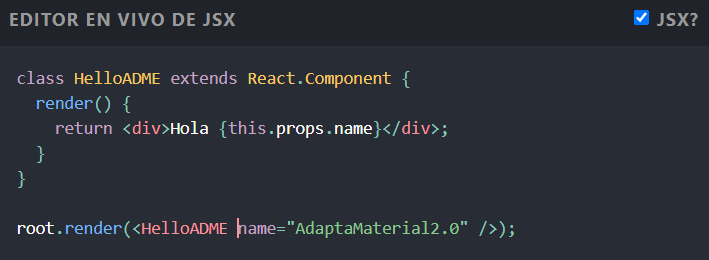
\includegraphics[width=0.6\textwidth]{Herraientas_Empleadas/ReactJSX.PNG}
    \caption{Componente con JSX.}
    \label{JSX}
  \end{subfigure}

  \begin{subfigure}{\textwidth}
    \centering
    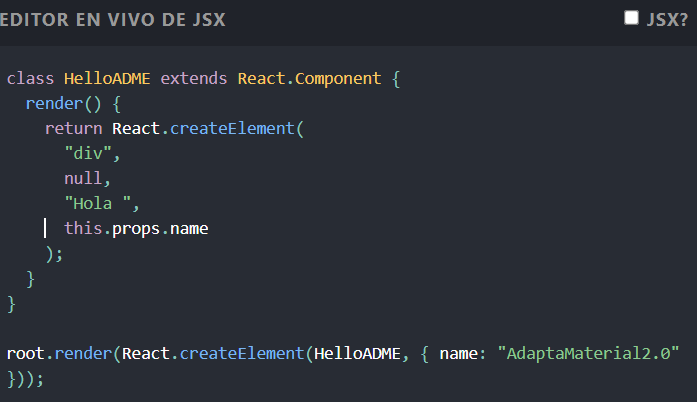
\includegraphics[width=0.6\textwidth]{Herraientas_Empleadas/ReactSinJSX.PNG}
    \caption{Componente sin JSX.}
    \label{SJSX}
  \end{subfigure}
  \caption{Componentes React}
  \label{fig:react}
\end{figure}

En los componentes de React se utiliza Tailwind CSS, una librería de estilos CSS, para la construcción rápida de interfaces de usuario sin tener que escribir CSS personalizado para cada elemento. En la siguiente subsección se hablará de ella.



\section{Tailwind CSS}\label{sec:tailwind}
Tailwind CSS\footnote{\url{https://tailwindcss.com/}} es un framework CSS que permite aplicar estilos predefinidos directamente en el HTML sin tener que crear y manejar archivos CSS propios para conseguir un estilo concreto. Hemos decidido utilizar este framework porque facilita la labor de dar estilo al HTML de la página, debido a que no tenemos que pensar en que clases o identificadores dar a los elementos HTML y, por lo general, tampoco necesitamos gestionar un archivo CSS por cada página o componente de React. Otra de las razones por las que hemos escogido este framework frente a otros muy parecidos, como Bootstrap\footnote{\url{https://getbootstrap.com/}}, es la facilidad que ofrece para personalizarlo y adaptarlo a nuestras necesidades. En el caso de Bootstrap, necesitas utilizar SASS o crear tus propios archivos CSS para poder personalizar el estilo, mientras que en Tailwind CSS modificando un archivo de configuración puedes personalizar/añadir colores, añadir distintos tipos de fuente de texto, añadir distintos tamaños de letra, etc. Otras ventajas que ofrece son:
\begin{itemize}
  \item \textbf{Rendimiento}: Tailwind elimina automáticamente todo el CSS que no se utilice a la hora de desplegar en producción la aplicación, consiguiendo que el paquete de CSS que se envía al cliente sea lo más pequeño posible.
  \item \textbf{Diseño responsive}: Permite aplicar distintos estilos dependiendo del tamaño de la ventana sin necesidad de pelearse con \textit{media queries}\footnote{\url{https://developer.mozilla.org/en-US/docs/Web/CSS/Media_Queries/Using_media_queries}} de CSS.
  \item \textbf{Reutilización}: Tailwind permite reutilizar conjuntos de utilidades que se repitan mucho definiendo una clase CSS propia que los aplique todos. Aun así, nosotros no utilizaremos, principalmente, el método que ofrece Tailwind para reutilizar estilos, ya que podemos conseguir el mismo resultado creando un componente de React, con la ventaja de poder añadir lógica de JavaScript.
\end{itemize}

% TODO: Añadir ejemplos de uso

\section{Slate}\label{sec:Slate}
Slate\footnote{\url{https://docs.slatejs.org/}} es un framework de JavaScript de código abierto que tiene como finalidad la creación de editores de texto personalizados "What You See Is What You Get" (WYSIWYG). Es la herramienta ideal para este proyecto, el cual busca construir un editor de texto de alta calidad capaz de realizar diversos tipos de adaptación curricular. A diferencia de las bibliotecas de edición de texto convencionales, Slate utiliza una estructura de árbol de datos para representar el contenido del editor, y proporciona una API para manipular dicho contenido de forma más efectiva.Las principales características de Slate incluyen:
\begin{itemize}
  \item \textbf{Personalización}: La biblioteca permite a los desarrolladores personalizar el editor de texto según sus necesidades, lo que significa que pueden definir sus propios tipos de nodos y componentes de renderizado.
  \item \textbf{Flexibilidad}: Al ser una biblioteca de JavaScript, SlateJS es altamente flexible y puede integrarse fácilmente con otras bibliotecas y marcos como React.
  \item \textbf{Rendimiento}: La estructura de árbol de datos utilizada por SlateJS permite que la biblioteca realice actualizaciones eficientes del DOM, lo que resulta en un editor de texto rápido y fluido.
  \item \textbf{Soporte de complementos}: Los complementos de SlateJS son módulos que proporcionan una funcionalidad adicional al editor de texto. Estos complementos pueden personalizarse y utilizarse según las necesidades del desarrollador.
  \item \textbf{Compatibilidad multiplataforma}: SlateJS es compatible con una amplia gama de navegadores y plataformas.
\end{itemize}

Slate es utilizado por variedad de aplicaciones web como, por ejemplo:
\begin{itemize}
  \item \textbf{Discord}: Utiliza Slate para sus canales de comunicación para colaborar y compartir.
  \item \textbf{Eraser}: Una aplicación web de borrador de fondos que utiliza Slate para permitir a los usuarios escribir y editar el texto en su sitio web.
  \item \textbf{GitBook}: Es una plataforma de creación y publicación de libros electrónicos que utiliza Slate como editor de texto para que los autores puedan escribir y editar sus libros.
\end{itemize}
\chapter{Metodología}\label{cap:metodologia}
En este capítulo se explicará la metodología de desarrollo utilizada (Sección \ref{cap:Kanban}) y se describirán las medidas tomadas para asegurar la calidad del software (Sección \ref{sec:qa}).

\section{Metodología de desarrollo}\label{cap:Kanban}
Para el desarrollo de este trabajo hemos decidido aplicar la metodología Kanban. Esta metodología tiene cuatro reglas básicas: visualizar el flujo de trabajo, determinar y respetar el límite de trabajo en curso (WIP), gestionar el flujo y hacer políticas explícitas. Estas reglas las hemos desarrollado en las siguientes subsecciones.

\subsection{Visualizar el flujo de trabajo: Tablero Kanban}\label{sec:flujoTrabajo}
En el proyecto hemos distinguido dos tipos de tareas, las tareas relacionadas con la memoria y las de implementación. Para el tablero Kanban hemos decidido crear cinco columnas: \textit{To Do}, \textit{Doing}, \textit{Testing}, \textit{Validate} y \textit{Done}.  Las tareas se irán moviendo a través del tablero teniendo en cuenta las siguientes definiciones de las columnas:
\begin{itemize}
  \item \textbf{\textit{To Do}}: Listado de todas las tareas sin empezar.
  \item \textbf{\textit{Doing}}: Tareas que se encuentran en desarrollo.
  \item \textbf{\textit{Testing}}: Una vez desarrollada la tarea, se probará que cumpla con los requisitos.
        Para las tareas de documentación el testing será realizado por todos integrantes del equipo siguiendo los siguientes pasos:
        \begin{enumerate}
          \item Cuando haya una tarea de memoria en dicha columna, esta dispondrá de una lista con \textit{checkboxes} con los nombres de los integrantes.
          \item Cuando un miembro del equipo haya terminado de revisar la tarea debe marcarlo en el \textit{checkbox} referido a él.
          \item Cuando todos los miembros del equipo hayan revisado la tarea, el ultimo revisor se encargará de mover la tarea a la columna de \textit{Validate}.
        \end{enumerate}
        Para las tareas de código, si se encuentra un error en una funcionalidad, ya sea durante esta fase o tras haberse dado por terminada, se creará una nueva tarea de tipo \textit{bug} en la columna \textit{To Do}.
  \item \textbf{\textit{Validate}}: Tareas a la espera de que sean validadas por las tutoras.
  \item \textbf{\textit{Done}}: Tares finalizadas
\end{itemize}
En la Figura \ref{fig:taleros} se muestra la evolución del Tablero Kanban a lo largo del proyecto.
\begin{figure}[ht!]
  \centering
  \begin{subfigure}{\textwidth}
    \centering
    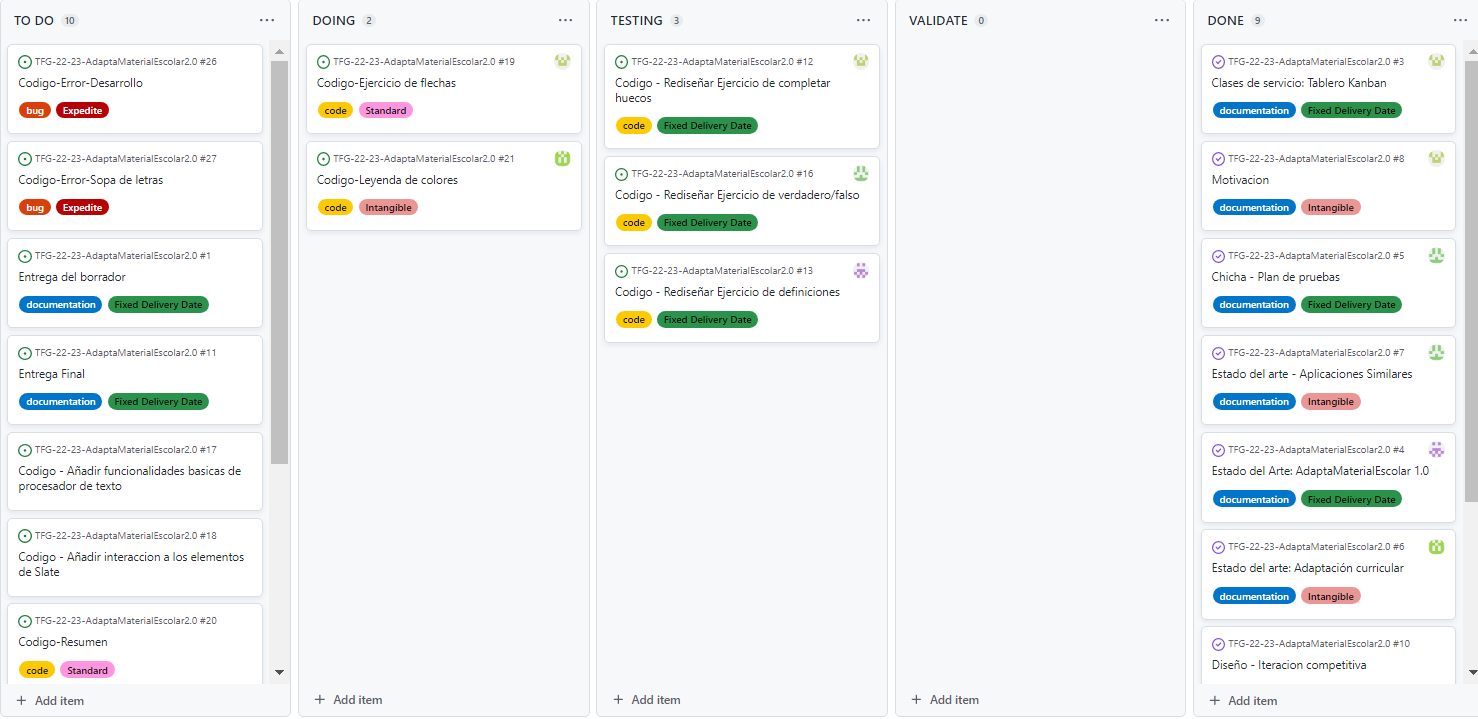
\includegraphics[width=0.8\textwidth]{Tablero/25-02-2023.PNG}
    \caption{Tablero Kanban 25-02-2023.}
    \label{fig:tabFeb}
  \end{subfigure}

  \begin{subfigure}{\textwidth}
    \centering
    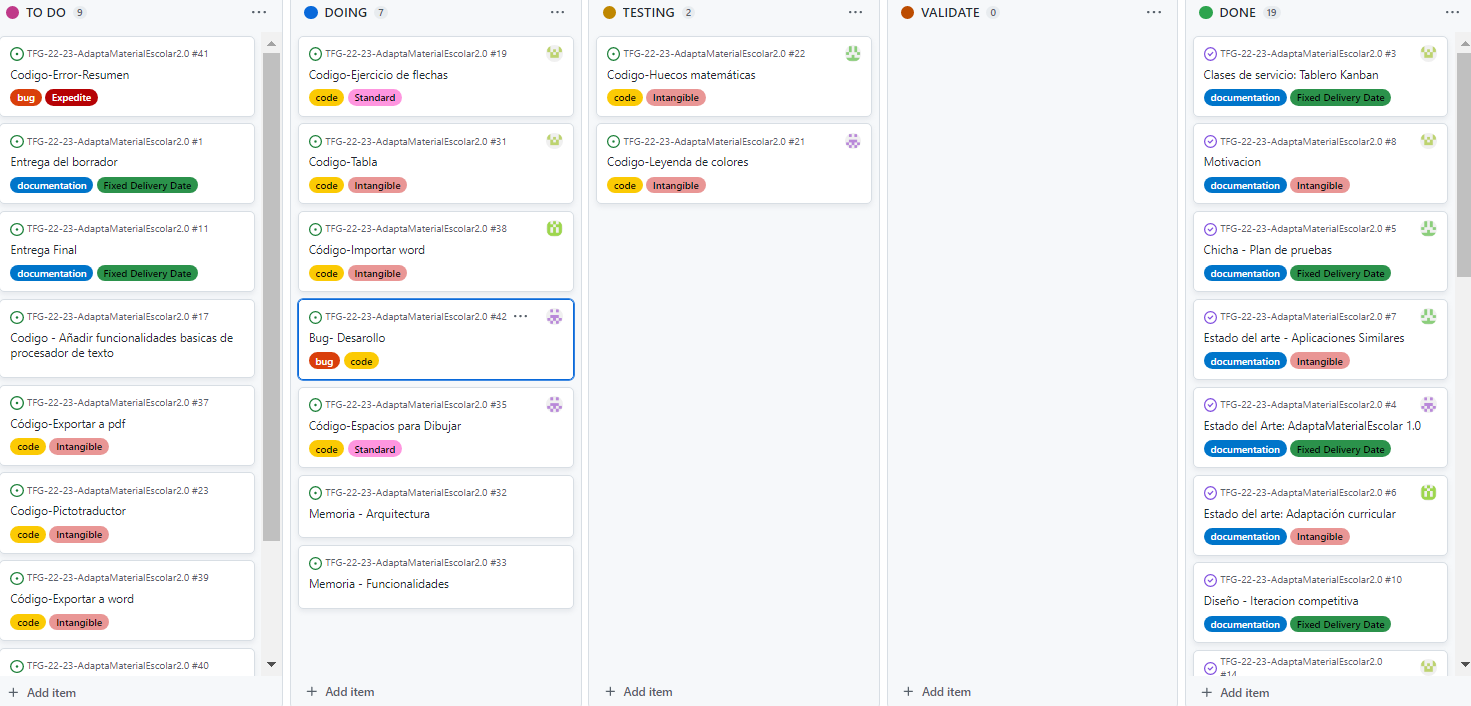
\includegraphics[width=0.8\textwidth]{Tablero/27-03-2023.PNG}
    \caption{Tablero Kanban 27-03-2023.}
    \label{fig:tabmarzo}
  \end{subfigure}

  \begin{subfigure}{\textwidth}
    \centering
    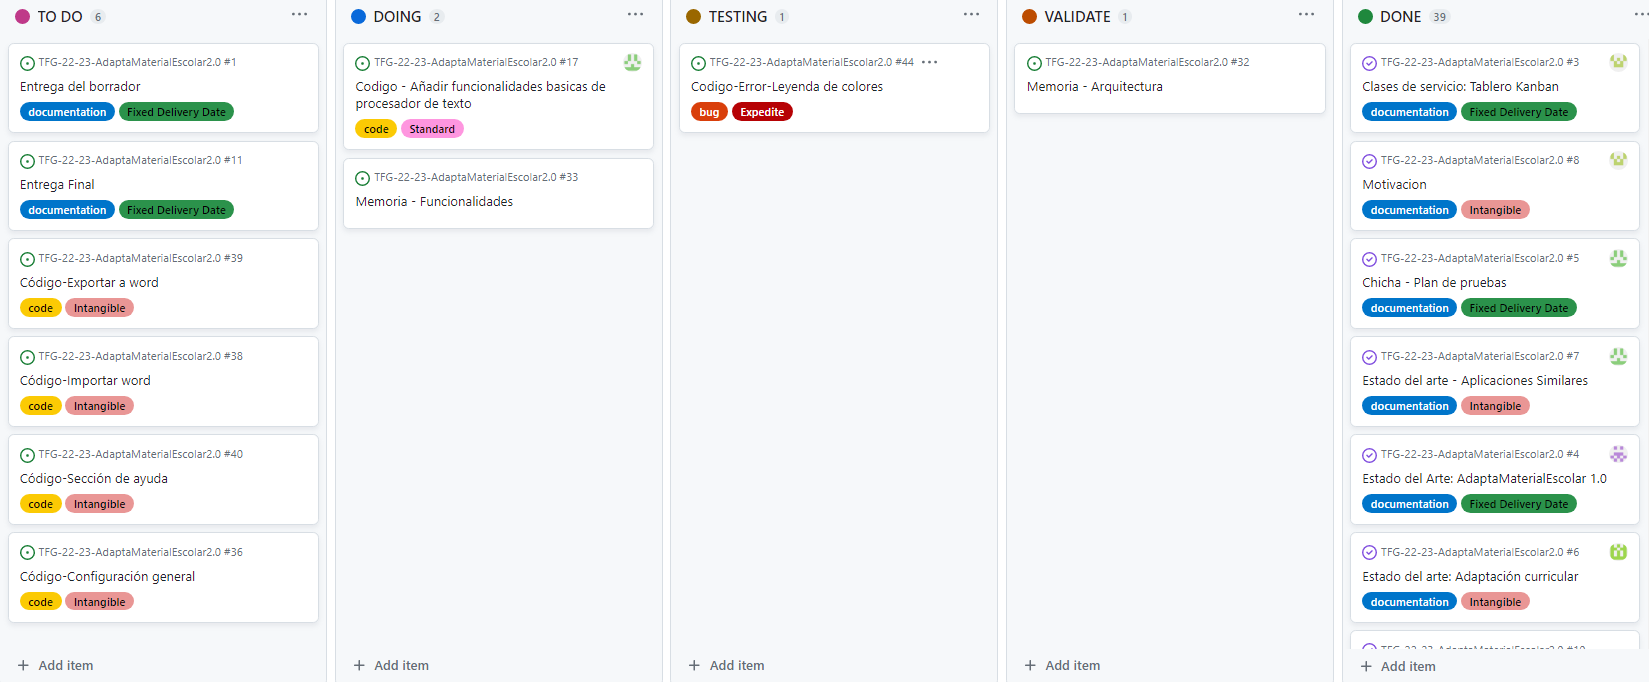
\includegraphics[width=0.8\textwidth]{Tablero/4-05-2023.PNG}
    \caption{Tablero Kanban 4-05-2023.}
    \label{fig:tabmayo}
  \end{subfigure}

  \caption{Tablero Kanban.}
  \label{fig:taleros}
\end{figure}

\subsection{Políticas explícitas}
\label{sec:politicas}
A continuación se presentan las políticas explicitas que hemos ido estableciendo a lo largo del proyecto:

\begin{itemize}
  \item Límites del trabajo en curso (WIP): en las columnas de \textit{Doing} y \textit{Testing} habrá como máximo 2 tareas por persona en cada columna, es decir, no podrá haber más de 8 tareas en cada una de esas columnas.
  \item Definición de \textit{Done}:
        \begin{itemize}
          \item Tareas de memoria: Cuando hayan sido validadas por las tutoras.
          \item Tareas de implementación: Cuando hayan pasado todo el plan de pruebas.
        \end{itemize}
  \item Cuando un integrante del grupo haya terminado su tarea él será el encargado de moverla a la columna correspondiente.
  \item Cualquier integrante del grupo puede poner una tarea en el tablero tras consultarlo con el resto.
  \item Todos los domingos a las 12:00 habrá reunión de equipo para poner en común el trabajo realizado por cada miembro.
  \item Se realizará una reunión de todos los integrantes una semana antes de la revisión con las tutoras para comprobar el trabajo realizado por cada miembro del equipo.
\end{itemize}

\subsection{Clases de servicios}
\label{claseDeServicio}
En Kanban para priorizar las tareas del tablero en ocasiones se emplean las clases de servicio. Estas son una serie de categorías que nos son útiles para clasificar cada una de las tareas de nuestro sistema, las cuales nos permiten identificar rápidamente el nivel de prioridad que tiene la tarea sin hacer un análisis o estimación muy extensa del mismo. Además, la categoría asociada a una tarea determinará como se desplazará la tarea en el tablero. En nuestro caso las clases de servicio que empleamos son las siguientes:
\begin{itemize}
  \item Expedite: Tareas que necesitan ser gestionadas de manera acelerada o urgente. Por ejemplo, algún problema con el editor que nos impediría implementar cualquier otra tarea hasta que esta esté terminada.
  \item Fixed Delivery Date: Tareas con fecha fija que debemos cumplir. Por ejemplo, la corrección de la documentación para la siguiente reunión con las tutoras.
  \item Standard: Tareas que ya ha hecho antes el equipo que no tienen una fecha fija y que ya saben como realizar. Por ejemplo, la realización de pruebas de control de calidad de rutina en el software.
  \item Intangible: Tareas que son nuevas para el equipo, tareas que nunca antes han realizado y por tanto, se desconoce el tiempo que se le va a dedicar y el riesgo que suponen. Por ejemplo, la función de exportar a PDF.
\end{itemize}

Para su aplicación tomaremos unas medidas en base a su prioridad. Las clases \textit{Expedite} son las más prioritarias por lo que serán las primeras en ser realizadas. Las \textit{Fixed Delivery Date} serán las siguientes, si en su debida fecha (la cual estará indicada en su descripción) no están implementadas, se convierten en \textit{Expedite} (pasaran a ser más prioritarias). Las \textit{Standard} son un poco menos prioritarias que las \textit{Fixed Delivery Date} al contar con el coste y el esfuerzo que suponen pero presentan un cierto grado de incertidumbre al no tener una fecha fija. Por último, se elegirán las \textit{Intangibles} su prioridad varía al presentar un alto grado de incertidumbre, ya que inicialmente se desconoce el riesgo que suponen pero pueden convertirse en \textit{Standard} o en \textit{Expedite}.

\section{Aseguramiento de la Calidad (QA)}\label{sec:qa}
En está sección se explican las medidas que se han tomado en el proyecto para asegurar la calidad del software. La importancia de un formato consistente y limpio del código fuente se explica en la Sección \ref{sec:qaformato}, el uso de la técnica de análisis linting para detectar errores antes de la ejecución de la aplicación se cuenta en la Sección \ref{sec:qalinting} y el plan de pruebas que se ha seguido en el proyecto para asegurar el correcto funcionamiento de la aplicación esta en la Sección \ref{sec:qapruebas}.

\subsection{Formato del código}\label{sec:qaformato}
Cuando varios desarrolladores trabajan en un proyecto, es común que tengan diferentes estilos de escritura de código, lo que puede dificultar la lectura y el mantenimiento de este. Para mejorar la calidad del código se ha decidido utilizar una herramienta para dar formato al código. Esta herramienta permite mantener un estilo consistente y limpio, facilitando la lectura del código escrito por otros miembros del equipo ya que no es necesario habituarse al estilo de cada uno.

Para ello vamos a utilizar la herramienta Prettier explicada en la Sección \ref{sec:prettier}.

\subsection{Linting}\label{sec:qalinting}
El linting es una técnica de análisis estático de código que busca errores de programación, inconsistencias y malas prácticas en el código fuente. En otras palabras, es una técnica de control de calidad que ayuda a los desarrolladores a identificar y corregir errores en su código antes de que sea utilizado en producción. Con el uso del Linting se pueden detectar errores de sintaxis, ``malas prácticas'' y código poco intuitivo o difícil de mantener.

Con este fin hemos usado en el proyecto la herramienta ESLint explicada en la Sección \ref{sec:eslint}.

\subsection{Plan de Pruebas}\label{sec:qapruebas}
Para asegurar el correcto funcionamiento del software construido se ha decidido realizar pruebas manuales, ya que se ha considerado que para el tamaño actual del proyecto no supone un problema realizar pruebas manuales para comprobar las distintas funcionalidades. Si, en un futuro, se decide extender la aplicación y añadir más funcionalidades es recomendable actualizar este plan de pruebas, incluyendo pruebas automatizadas e integración continua. Las pruebas de una tarea de implementación concreta las realizará algún miembro del equipo que no haya participado en el desarrollo de esta y las hará cuando la tarea se encuentre en la columna de \textit{Testing}. La ventaja de que las pruebas las realice un miembro que no se haya visto involucrado en el desarrollo de la tarea es que puede sacar más casos de prueba que aquellos miembros que han implementado la tarea y conocen el código.

Cuando un miembro del equipo se haya asignado una tarea de implementación para probar, tendrá que seguir los siguientes pasos:
\begin{enumerate}
  \item \textbf{Generación de los casos de prueba}: Se realizará una tabla con los distintos casos de prueba que se utilizarán para probar una funcionalidad concreta, teniendo en cuenta los requisitos de usuario. Los casos de prueba se entienden como las condiciones de ejecución (precondiciones), el conjunto de entradas, el objetivo de la prueba (campos y condiciones que se quieren comprobar) y los resultados esperados tras ejecutar la prueba (postcondiciones). En la Tabla \ref{tab:ejemplocasosprueba} se muetra un ejemplo de los casos de prueba utilizados en el proyecto.
  \item \textbf{Definición de los procedimientos de la prueba}: Después de generar los casos de prueba, se definirá un guion en el que se explicarán los pasos a seguir para la ejecutar la prueba. En este guion se deben tener en cuenta todos los casos de prueba generados anteriormente. Cada paso debe ser claro y concreto, además de ofrecer ejemplos de datos de entrada, por ejemplo ``Escribir `hola'\, en el campo de añadir frase.'' o ``Pulsar botón de añadir frase.''.
  \item \textbf{Ejecución de la prueba}: Una vez se hayan definido los pasos necesarios para probar una funcionalidad concreta, hay que ejecutar la prueba, siguiendo estos pasos. Durante la ejecución, se registrarán los resultados obtenidos que no concuerden con los resultados esperados o comportamientos de la funcionalidad que puedan afectar negativamente a la experiencia de usuario.
  \item \textbf{Realización del informe de prueba}: Finalmente, en caso de que al realizar la prueba se hayan encontrado fallos, se deberá crear una incidencia de tipo \textit{bug} con la clase de servicio \textit{Expedite}. En la descripción de esta incidencia se deberá informar de los resultados obtenidos, los resultados esperados y los pasos a seguir para replicar cada fallo o problema que haya ocurrido durante la ejecución de la prueba. También se puede incluir información que pueda ser relevante para encontrar una solución a cada fallo o problema. En la Figura \ref{fig:ejemploerrores} se muetra un ejemplo de una incidencia con los errores encontrados tras ejecutar el plan de pruebas. En caso de no haber encontrado errores, se cerrará la incidencia del desarrollo de la funcionalidad que se está probando.
\end{enumerate}

\begin{table}[H]
  \resizebox{1.1\textwidth}{!}{
    \begin{tabular}{|c|c|c|c|c|}
      \hline
      \textbf{Precondición}       & \textbf{Campo}   & \textbf{Condición}                                             & \textbf{Datos de entrada}   & \textbf{\begin{tabular}[c]{@{}c@{}}Salida esperada\\ (Postcondición)\end{tabular}} \\ \hline
      Lista={[} {]}               & Nueva frase      & Longitud de frase \textless{}= 0                               & Frase = “”                  & Lista = {[} {]}                                                                    \\ \hline
      Lista={[} {]}               & Nueva frase      & Longitud de frase \textgreater 0                               & Frase = “hola”              & Lista = {[}“hola” {]}                                                              \\ \hline
      Lista={[}“hola”{]}          & Editar frase     & Longitud de frase \textless{}= 0 y la Frase existe en la lista & Frase = “”                  & Lista = {[}“hola”{]}                                                               \\ \hline
      Lista={[}“hola”{]}          & Editar frase     & Longitud de frase \textgreater 0 y la Frase existe en la lista & Frase = “adios”             & Lista = {[}“adios”{]}                                                              \\ \hline
      Lista={[}“hola”{]}          & Borrar frase     & Existe la frase a borrar en la lista                           & Frase = “hola”              & Lista = {[} {]}                                                                    \\ \hline
      Lista={[}“hola”, “adios”{]} & Reordenar frases &                                                                & Lista={[}“hola”, “adios”{]} & Lista = {[}“adios”, “hola”{]}                                                      \\ \hline
      Lista={[}{]}                & Reordenar frases &                                                                & Lista={[}{]}                & Lista={[}{]}                                                                       \\ \hline
      Lista={[}“hola”{]}          & Reordenar frases &                                                                & Lista={[}“hola”{]}          & Lista={[}“hola”{]}                                                                 \\ \hline
    \end{tabular}
  }
  \caption{Ejemplo de casos de prueba (Funcionalidad verdadero/falso).}
  \label{tab:ejemplocasosprueba}
\end{table}

\begin{figure}[ht!]
  \centering
  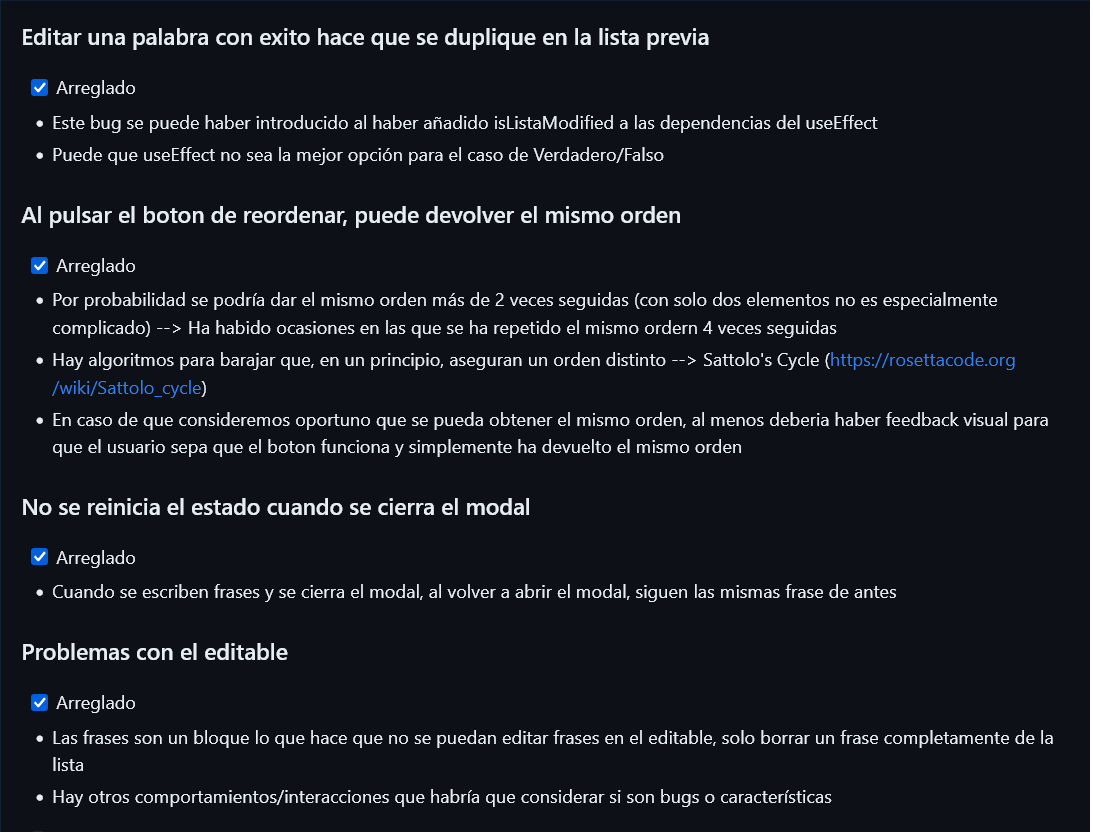
\includegraphics[width=1\textwidth]{QA/ErroresVF.png}
  \caption{Incidencia de errores (Funcionalidad verdadero/falso).}
  \label{fig:ejemploerrores}
\end{figure}

Los casos de prueba, guiones de prueba y errores encontrados de cada funcionalidad se muestran en el Apéndice \ref{ape:pruebas}.
\chapter{AdaptaMaterialEscolar 2.0}
\label{cap:AdaptaMaterialEscolar2.0}
En este capítulo explicaremos la obtención de requisitos y cómo se han clasificado en la Sección \ref{cap:requisitos}. También se describirá el diseño realizado por cada integrante de la aplicación para la iteración competitiva y el diseño final de las funcionalidades en la Sección \ref{disenyoDeLaAplicacion}.


\section{Requisitos}
\label{cap:requisitos}

Lo primero que hicimos fue analizar la memoria de AdaptaMaterialEscolar 1.0 \citep*{AdaptaMaterialEscolar1.0}extrayendo las funcionalidades que faltaban por implementar y los resultados de la evaluación que se realizó. Tras este análisis hemos decidido agrupar las nuevas funcionalidades según los datos sobre los que trabajan y las acciones que realizan.

De esta forma han surgido las siguientes agrupaciones: formato (funcionalidades que tienen relación con el estilo o la estructura del documento), ejercicios (funcionalidades relacionadas con la creación de actividades) y auxiliar (resto de funcionalidades que no pertenecen a formato o a ejercicios). Quedan así las funcionalidades agrupadas de la siguiente manera:
\\

\begin{itemize}
  \item Funcionalidades relacionadas con el formato:
        \begin{itemize}
          \item Añadir encabezado al texto: El usuario eligirá un encabezado que se añadirá al documento de trabajo.
          \item Añadir un tipo de fuente escolar: Incluir en los tipos de fuentes la escolar. Dicha fuente se refleja en la Figura \ref{escolar}.
                \begin{figure}[ht!]
                  \centering
                  
\includegraphics[scale=0.3]{AdaptaMaterialEscolar/FunteEscolar.png}
                  \caption{Fuente escolar.}
                  \label{escolar}
                \end{figure}
          \item Añadir una leyenda de colores: Sirve para que el docente pueda poner de distintos colores distintas palabras según la categoría a la que pertecenecen, por ejemplo sustantivos en rojo y adjetivos en verde.
          \item Añadir leyenda de colores para el tema de cada asignatura: Dar la posibilidad de que cada asignatura tenga un color. Al crear un documento según la asignatura se pondrá el borde del documento del color que corresponde a dicha asignatura.
          \item Añadir cuadrícula: En vez de renglones de una única línea se podrá poner para responder a una pregunta la cuadrícula.
          \item Añadir la opción de añadir doble pauta: En vez de renglones de una única línea se podrá poner para responder a una pregunta la doble pauta.
          \item Estandarizar formato para títulos e índices del temario: Dar la opción de crear estilos para estandarizar documento de trabajo.
          \item Enumerar ejercicios de forma automática: Establecer un orden numérico para los ejercicios de forma automática según se van creando para que el usuario no se tenga que preocupar de ese aspecto.
        \end{itemize}

  \item Funcionalidades asociadas con la creación de ejercicios:
        \begin{itemize}
          \item Ejercicios de relacionar contenido mediante flechas: Generar un ejercicio para relacionar conceptos mediante flechas.
          \item Añadir ejercicios de cálculo con huecos a rellenar por el alumno: Posibilidad de introducir ejercicios de cálculo con espacios en blanco para que el alumno rellene dichos huecos con contenido adecuado.
          \item Añadir ejercicios con espacio para dibujar: Añadir amplio hueco en blanco con el fin de que el alumno pueda dibujar.
          \item Ejercicios de completar los espacios en blanco en tablas y esquemas: Dada una tabla o un esquema se establecen espacios en blanco para que el alumno los rellene con el contenido adecuado.
        \end{itemize}

  \item Funcionalidades auxiliares:
        \begin{itemize}
          \item Generar un resumen a partir de un texto.
          \item Exportar el documento a formato Word.
          \item Añadir un pictotraductor: Que permita dada una frase traducirla a pictogramas.
          \item Añadir imágenes buscando una palabra: A partir de una palabra se busca su respectiva imagen en las bases de datos de imágenes libres.
          \item Sustituir una palabra por una imagen: Dado un texto esta funcionalidad permitirá que se seleccione una palabra, se busque una imagen asociada a dicha palabra y esta se reemplazará por la imagen seleccionada.
          \item Crear una herramienta de recorte de imágenes: Tras seleccionar una imagen se dará la opción de quitar partes de la misma.
          \item Crear tablas que organicen el temario y/o las actividades, seleccionando contenido: Tras la selección de contenido por parte del usuario se creará una tabla en base a la información seleccionada, con un formato predefinido.
          \item Creación de esquemas.
        \end{itemize}

\end{itemize}


Tras haber analizado en detalle las funcionalidades anteriores hemos encontrado que varias de ellas ya están implementadas en la versión original de AdaptaMaterialEscolar y otras hemos decidido no implementarlas actualmente ya que consideramos que no tenemos la información suficiente para ello, pero las realizaremos una vez podamos reunirnos con los usuarios finales y obtener más información sobre ellas. El resto de funcionalidades son las que implementaremos en este proyecto.

Las siguientes funcionalidades son las que ya están implementadas en la versión original:
\begin{itemize}
  \item Añadir encabezado al texto: El documento de trabajo tiene una opción con una lista de encabezados para añadir uno y cuando se pulsa un encabezado el documento de trabajo convierte el formato de la letra en el del encabezado seleccionado.
  \item Enumerar ejercicios de forma automática: El documento de trabajo permite añadir listas enumeradas.
\end{itemize}
Las funcionalidades que hemos decidido descartar de momento por falta de información son las siguientes:
\begin{itemize}
  \item Añadir imágenes buscando una palabra. Partimos de que debemos usar una base de datos de imagen libre pero no tenemos la información suficiente para definir cuál sería la base de datos correcta.
  \item Sustituir una palabra por una imagen. No la realizaremos ya que no tenemos claro de dónde obtener las imágenes ni el estilo de estas.
  \item Crear una herramienta de recorte de imágenes para el texto original: No la realizaremos ya que no tenemos claro qué tipo de recorte tenía pensado el usuario.
  \item Crear tablas que organicen el temario y/o las actividades, seleccionando contenido: Descartamos dicha funcionalidad ya que no tenemos la información suficiente del formato que desea el usuario.
  \item Crear esquemas: Descartamos dicha funcionalidad ya que no tenemos la información suficiente del formato que desea el usuario.
  \item Ejercicios de completar los espacios en blanco en tablas y esquemas. Descartamos esta funcionalidad ya que depende de la funcionalidad de crear tablas y esquemas.
\end{itemize}

Por lo tanto, las funcionalidades que vamos a implementar son las que se muestran a continuación:


\begin{itemize}
  \item Generar un resumen a partir de un texto con el fin de ayudar a un alumno a comprender los elementos claves del texto de manera mas rápida.
  \item Exportar el documento a formato Word para hacer modificaciones y que el usuario pueda continuar con las modificiones del documento.
  \item Añadir un pictotraductor con el fin de trasformar un texto a su equivalente en pictogramas para que el alumno pueda adquirir nuevos conocimientos de forma más sencilla.
  \item Ejercicios de relacionar contenido mediante flechas ya que ayuda al alumno a consolidar conceptos.
  \item Añadir un tipo de fuente escolar con el fin de facilitar la lectura y la escritura al alumno.
  \item Añadir una leyenda de colores con la categoría de cada tipo con el fin de  ayudar al alumno a relacionar conceptos.
  \item  Añadir ejercicios de cálculo con huecos a rellenar por el alumno para que el alumno practique el cálculo.
  \item  Añadir ejercicios con espacio para dibujar con el fin de que el alumno pueda reflejar lo que piensa, interpreta y representa sobre algo.
  \item Añadir leyenda de colores para el tema de cada asignatura con el fin de que el alumno pueda distinguir entre las asignaturas.
  \item Añadir cuadrícula para escribir los números con el fin de facilitar los ejercicios de matemáticas.
  \item Añadir la alternativa de añadir doble pauta con el fin de que el alumno adquiera un tamaño de letra adecuado.
  \item Estandarizar formato para títulos e índices del temario con el fin de que el profesor pueda definir un estilo.

\end{itemize}

\section{Diseño de la aplicación}
\label{disenyoDeLaAplicacion}
Analizando la interfaz de AdaptaMaterialEscolar 1.0 hemos llegado a la conclusión de que la experiencia de usuario no era cómoda. Por ejemplo, obligaba a cargar un PDF y las funcionalidades se abrían en una ventana bastante pequeña. Además, la selección de colores no nos pareció la adecuada y el estilo general de la aplicación no era moderno. Por todo lo anterior decidimos rediseñar la aplicación.

Para el rediseño hemos realizado una iteración de diseño competitiva. Esta trata de la creación, por parte de cada integrante, de un nuevo diseño de la aplicación y la puesta en común de los diseños para debatir sobre qué sería lo óptimo e intuitivo para el usuario. Luego junto a las tutoras realizamos un \textit{brainstorming} basándonos en dichos diseños. Por último, construimos el diseño final de la aplicación.

A continuación, se explicará el diseño de la aplicación por parte de cada integrante y el diseño final de la aplicación.
\subsection{Diseño de los integrantes}
En esta sección se explicará los diseños creados por cada integrante junto a las imágenes de los mismos. Todos los diseños mencionados se encuentran en el Apéndice \ref{cap:anexo}, en las secciones \ref{sec:disenyoAlvaro}, \ref{sec:disenyoDunia}, \ref{sec:disenyoAlberto}, \ref{sec:disenyoJohan}.

\subsubsection{Álvaro Gómez Sittima}
Para empezar, diseñé la página de inicio \ref{fig:disenyoAlvaro01} la cual dispone de un menú superior con el logo de la aplicación a la izquierda y enlaces a las distintas páginas de la aplicación (Ayuda y Contacto) a la derecha. Este menú superior aparecerá en todas las páginas de la aplicación y se utilizará el logo de la aplicación como enlace a la página de inicio. En esta página el usuario podrá cargar un fichero PDF y utilizar un editor de documentos para poder adaptar el material del PDF. El acceso a las opciones de archivo, formato y adaptaciones se encontrarán como botones integrados en la barra de herramientas del editor de documentos. Además, también se mostrarán opciones relevantes en un barra de herramientas flotante encima del texto que tenga seleccionado en el PDF o en el editor de documentos. El diseño de esta página sin un PDF cargado se puede ver en la Figura \ref{fig:disenyoAlvaro01} y con un PDF cargado en la Figura \ref{fig:disenyoAlvaro02}. Si el usuario pulsa el enlace de ayuda en el menú superior, este le llevará a la página de ayuda la cual dispondrá de un buscador, con el que podrá buscar información sobre un tema en concreto relacionado con el uso de la aplicación. Si no se realiza una búsqueda aparecerán todos los temas sobre los que se ofrece ayuda. Cada tema aparecerá en una tarjeta con información sobre el tema y un breve video para apoyar lo explicado en la información.

En cuanto a las funcionalidades, realicé los siguientes diseños:
\begin{itemize}
  \item \textbf{Generar resumen}: En caso de que el usuario tenga texto seleccionado, cuando pulse la opción de generar resumen le saldrá una pequeña ventana encima con un campo para introducir el número de palabras del resumen y un botón para generar el resumen, llevandolo al documento de trabajo. En la Figura \ref{fig:disenyoAlvaro03} se muestra el diseño de esta funcionalidad en caso de tener texto seleccionado. En caso de no tener texto original, se abrirá una ventana aparte donde el usuario podrá escribir el texto a resumir y resumirlo.
  \item \textbf{Pictotraductor}: En caso de que el usuario tenga texto seleccionado, cuando pulse la opción de pictotraductor se traducirá automáticamente el texto a pictogramas y se llevará al documento de trabajo. Si pulsa alguno de los pictogramas generados podrá cambiarlo por otro. En la Figura \ref{fig:disenyoAlvaro04} se muestra el diseño de esta funcionalidad en caso de tener texto seleccionado. En caso de no tener texto original, se abrirá una ventana aparte donde el usuario podrá escribir el texto y traducirlo.
  \item \textbf{Definir huecos}: En caso de que el usuario tenga texto seleccionado, cuando el usuario pulse la opción de definir huecos, se llevará automáticamente el texto al documento de trabajo y el usuario podrá definir los huecos seleccionando las palabras. En la Figura \ref{fig:disenyoAlvaro05} se muestra el diseño de esta funcionalidad en caso de tener texto seleccionado. En caso de no tener texto original, se abrirá una ventana aparte donde el usuario podrá escribir el texto y definir los huecos.
  \item \textbf{Buscar pictograma}: Cuando el usuario pulse la opción de buscar pictogramas en la barra de herramientas del editor, se abrirá una ventana modal con un buscador. Al pulsar el botón de buscar, se mostrarán todos los pictogramas relacionados con el texto introducido, debajo del buscador. El usuario podrá arrastrar los pictogramas que desee al documento de trabajo. En la Figura \ref{fig:disenyoAlvaro06} se muestra el diseño de esta funcionalidad.
  \item \textbf{Ejercicio de definiciones}: Cuando el usuario pulse la opción de crear ejercicio de definiciones en la barra de herramientas del editor, se creará un recuadro en el documento de trabajo donde el usuario podrá añadir los distintos conceptos a definir y el número de renglones de cada definición. Cuando haya terminado de crear el ejercicio podrá darle al botón de aceptar para que el ejercicio se inserte en el documento de trabajo. En la Figura \ref{fig:disenyoAlvaro07} se muestra el diseño de esta funcionalidad.
  \item \textbf{Sopa de letras}: Cuando el usuario pulse la opción de crear sopa de letras en la barra de herramientas del editor, se creará un recuadro en el documento de trabajo donde el usuario podrá definir el número de filas, el número de columnas y añadir las palabras a buscar en la sopa de letras. Cuando haya terminado de crear la sopa de letras podrá darle al botón de aceptar para que se inserte en el documento de trabajo.
  \item \textbf{Leyenda de colores}: Cuando el usuario pulse la opción de crear la leyenda de colores en la barra de herramientas del editor, se creará un recuadro en el documento de trabajo donde el usuario podrá añadir los distintos conceptos y asignarles un color, con un selector de colores, a cada uno. Cuando haya terminado de crear la leyenda podrá darle al botón de aceptar para que se inserte en el documento de trabajo.
\end{itemize}

\subsubsection{Dunia Namour Doughani}
Inicialmente realicé el diseño de la página principal, la cual dispone de una cabecera con el logo de la aplicación, un desplegable que contiene las funcionalidades y un botón que te redirige a la vista de ayuda. En la parte izquierda de esta página se encuentra el documento documento de trabajo y la zona de la derecha se encuentra dividida en dos secciones, una para incluir la funcionalidad elegida por el usuario y otra para insertar un PDF, ambas disponen de la posibilidad de aumentar o disminuir el tamaño de la ventana. Este diseño se puedo ver en la Figura \ref{dunia1} Con respecto a las funcionalidades, he realizado los siguientes diseños:
\begin{itemize}
  \item \textbf{Generar un resumen:} El diseño de esta funcionalidad consta de un recuadro en el que introduces el texto y al pulsar un botón se genera el resumen el cual es documento de trabajo. Para incluirlo en el documento de trabajo el usuario tendrá que darle a la opción de copiar y pegarlo en el documento de trabajo. Este diseño se puedo ver en la Figura \ref{dunia2}.
  \item \textbf{Pictotraductor:} Este diseño consta de un recuadro donde introduces el texto y al darle a un botón se generan los pictogramas. Para introducir los pictogramas en el documento de trabajo se podrá mediante la tecla CTRL + click arrastrar al documento de trabajo los pictogramas escogidos o arrastrando todos a la vez sin seleccionar ninguno. Este diseño se puedo ver en la Figura \ref{dunia3}.
  \item \textbf{Ejercicio de flechas:} Para este diseño había pensado en que el usuario visualizara dos tablas, cada tabla tendría un botón de añadir o eliminar filas, aquellas celdas que quedasen vacías se trasformarían en huecos. Al darle al botón de terminar se incluiría el ejercicio de tablas sin el borde de las tablas en el documento de trabajo, donde se encuentre el puntero. Este diseño se puedo ver en la Figura \ref{dunia4}.
  \item  \textbf{Leyenda de colores:} Este diseño consta de un rectángulo donde pones las palabras de la leyenda, al lado de la palabra hay una opción para seleccionar el color. Además, dispone de dos botones, uno para añadir más palabras y otro para eliminarlas. Una vez el usuario haya finalizado la leyenda de colores pasa a colocarse al final del documento en el lado derecho. Este diseño se puedo ver en la Figura \ref{dunia5}.
  \item  \textbf{Ejercicios de cálculo con huecos:} Este diseño dispone de una opción para elegir el tamaño de la expresión matemática, una vez elegido se muestra tanto huecos como el tamaño escogido, al darle a cada hueco se podrá escribir tanto un número como una operación aritmética elemental, al finalizar se incluirá la expresión matemática en el documento de trabajo donde se encuentre el puntero. Este diseño se puedo ver en la Figura \ref{dunia6}.
  \item  \textbf{Leyenda de colores para el tema de cada asignatura:} Al darle a esta opción se abrirá un menú con las asignaturas, al presionar sobre una asignatura el borde del documento de trabajo pasará a tener el color predeterminado de dicha asignatura.
\end{itemize}
No realicé los rediseños para las funcionalidades implementadas en AdaptaMaterialEscolar 1.0  ya que no sabía cómo mejorar el diseño de las funcionalidades.


\subsubsection{Alberto Alejandro Rivas}
En este caso, los diseños fueron realizados en una herramienta de diseño de interfaces de usuario llamada Figma, con el objetivo de poder obtener un resultado más detallado y tener en cuenta la paleta de colores.

Se ha intentado mantener la misma estructura y funcionalidad que en la aplicación existente, pero haciendo que la interfaz de usuario sea más profesional. Para esto se ajustó el diseño de la barra de navegación, los botones, el componente para seleccionar un fichero pdf, etc. En la pantalla principal hay una barra de navegación y un componente en el que se puede arrastrar o seleccionar un fichero pdf. Una vez seleccionado el archivo, se muestra otra página que se divide en dos, en una mitad está el pdf y en la otra está el editor de texto. Estos diseños se pueden observar en las figuras \ref{AlbertoPaginaPrincipal1} y \ref{AlbertoPaginaPrincipal2}. Por último, el usuario podrá acceder a cada funcionalidad haciendo click en los botones que se encuentran en la parte superior del editor.

Para hacer el diseño de las funcionalidades ya implementadas en AdaptaMaterial 1.0 también se ha utilizado la misma estructura, haciendo algunos ajustes para darles un estilo más profesional, pero manteniendo el mismo funcionamiento. En las figuras \ref{Alberto13}, \ref{Alberto14}, \ref{Alberto15}, \ref{Alberto16} y \ref{Alberto17} se muestran los diseños de estas funcionalidades.

A continuación se muestran los diseños de las nuevas funcionalidades que no estaban implementadas en AdaptaMaterial 1.0:

\begin{itemize}
  \item \textbf{Leyenda de colores:} consta de un input en el que se puede escribir el nombre de la categoría y un selector de colores para poder elegir el color que le corresponde. Una vez hecho esto, se puede hacer click en el botón con el símbolo de más para añadir la categoría a la lista. También hay una vista previa en la que se muestra cómo será el resultado. Este diseño se puede ver en la figura \ref{Alberto1}.
  \item \textbf{Leyenda de colores por asignatura:} consta de un selector de colores para elegir el color de la asignatura. Una vez seleccionado, a la página se le añadirá un borde de este color. Este diseño se puede ver en la figura \ref{Alberto2}.
  \item \textbf{Cuadrícula y doble pauta:} estas dos funcionalidades tienen un modal similar, en el que simplemente se selecciona el número de líneas que se quiere insertar en el documento de trabajo. Este diseño se puede ver en las figuras \ref{Alberto3} y \ref{Alberto4}.
  \item \textbf{Relacionar conceptos mediante flechas:} los inputs de texto se dividen en dos columnas y en estos se puede añadir el contenido que se quiere relacionar. También hay un botón en la parte inferior para añadir una nueva fila. Este diseño se puede ver en la figura \ref{Alberto5}.
  \item \textbf{Fórmulas matemáticas:} para este ejercicio simplemente hay un input en el que se puede escribir una fórmula matemática en LaTeX. Este diseño se puede ver en la figura \ref{Alberto6}.
  \item \textbf{Generar resumen y pictotraductor:} estas dos funcionalidades también tienen una interfaz similar. Simplemente hay un input en el que el usuario puede pegar el contenido que quiere resumir o traducir a pictogramas y al dar click en el botón de aceptar, se generará automáticamente a través de una API y se insertará el resultado en el documento de trabajo. Este diseño se puede ver en las figuras \ref{Alberto8} y \ref{Alberto10}.
  \item \textbf{Espacio para dibujar:} hay dos inputs, en los cuales se puede escribir la altura y anchura en centímetros que va a tener el espacio para dibujar. Al insertarse en el documento de trabajo, este espacio será simplemente un rectángulo vacío con un borde. Este diseño se puede ver en la figura \ref{Alberto7}.
  \item \textbf{Buscar imágenes:} el funcionamiento es igual al de la funcionalidad de buscar pictogramas. El usuario puede hacer una búsqueda y se le mostrarán todos los resultados encontrados, al darle click a uno de ellos, esta imagen se insertará en el documento de trabajo. Este diseño se puede ver en la figura \ref{Alberto12}.
\end{itemize}



\subsubsection{Johan Sebastian Salvatierra Gutierrez}
Para realizar el diseño de la aplicación realicé una división entre páginas y funcionalidades.
En primer lugar, las páginas. Para estas tuve de inspiración Youtube, donde se dividen en tres: página de inicio, página sobre nosotros y página de información. Comenzando con la página de inicio, con un editor de texto y una cabecera que dispone de un menú para moverte entre las páginas y un botón de configuración con forma de engranaje que permite elegir si tener un visualizador de PDF o una barra de funciones como se ve en la Figura \ref{Johan1}. Si el usuario decide personalizar la pantalla de inicio con el botón de configuración obtendra una pantalla similar a la mostrada en la Figura \ref{Johan2} donde podemos ver que el cuadrado izquierdo superior es el visualizador de PDF y el inferior es la barra de funciones y el cuadrado derecho es el editor de texto. Si el usuario decide usar el menú para cambiar de página aparecera un panel a la derecha que servirá como barra de navegación como se puede ver en la Figura \ref{Johan3}. Para la página de información el usuario dispondrá de una serie de videos didácticos y un buscador para conocer como explotar al máximo el potencial de AdaptaMaterialEscolar 2.0 (esto lo podemos ver en la Figura \ref{Johan4}). En cuanto a la página sobre nosotros, el usuario se encontrará con unos recuadros con forma de tarjeta con información de cada integrante (esto lo podemos ver en la Figura \ref{Johan5}).
En segundo lugar, las funcionalidades auxiliares aparecerán  como botones en el editor y las funcionalidades que no sean auxiliares aparecerán en el cuadrado mencionado anteriórmente y son las siguientes:
\begin{itemize}
  \item \textbf{Sopa de letras:} Sopa de letras: El usuario podrá elegir la cantidad de filas y columnas y luego introducir las palabras. Asimismo, se incluirán botones con signo de más y menos para añadir o eliminar palabras. También tendrá la opción de agregar un ejemplo de cómo resolver la sopa de letras a través de una casilla de verificación. Para generar, resetear o tener una vista previa, tendrá a su disposición botones. Todo esto se puede ver en la Figura \ref{Johan6}.
  \item \textbf{Picotraductor:} El usuario introducirá el texto para convertirlo en una representación en pictogramas. Luego tendrá que presionar el botón ``Generar'' y automáticamente se motrará el resultado como se puede ver en la Figura \ref{Johan7} y podrá arrastrarlos pictogramas al editor.
  \item \textbf{Ejercicio de flechas:} El usuario introducirá los conceptos en el orden que elija y podrá aumentar el número de columnas tendrá la opción de generar o resetear como se ve en la Figura \ref{Johan8}.
  \item  \textbf{Leyenda de colores:} El usuario podrá elegir el color del concepto y la descripción del concepto. Podrá modificarlos en cualquier momento y además podrá añadir y eliminar conceptos con su respectivo color, para generar el resultado o resetear los valores introducidos dispondrá de botones. Todo esto se puede ver en la Figura \ref{Johan9}. Este diseño es para la leyenda por conceptos y la leyenda de temas.
\end{itemize}
Por otra parte, las funcionalidades de pictograma, completar huecos, definiciones y desarrollo consideré emplear el diseño de AdaptaMaterialEscolar 1.0. Para la funcionalidad de verdadero o falso tendrá el mismo formato del ejercicio de flechas y el de generar un resumen tendrá el mismo formato del pictotraductor. En cuanto a las opciones de doble pauta, cuadrícula, estandarizar formato, espacio para dibujar, fuente escolar y convertir a formato Word se dispondrá de botones.


\subsection{Diseño final}\label{subsec:DisenyoFinal}
A continuación expondremos el diseño final de la aplicación. Para ello partimos de los diseños expuestos anteriormente. Todas las funcionalidades se han diseñado como ventanas modales para centrar la acción del usuario en la funcionalidad seleccionada y disponen de un boton \textit{OK} para confirmar la vista previa y transferir el ejercicio al documento de trabajo.


\subsubsection{Pantalla de inicio}
Ninguno de los diseños de los integrantes se han considerado razonables porque al tener el editor y el PDF a la vez hace que el usuario tenga menos espacio. Además, se pensó que tener el PDF al lado del editor solo para copiar contenido no aportaba ninguna ventaja respecto a tener el PDF en una ventana aparte. Otro problema fue la distribución del acceso a las agrupaciones de las funcionalidades. Inicialmente se pensó en ponerlas en el lateral izquierdo de la pantalla, pero eso volvía a quitar espacio al editor. Por ello lo descartamos y pensamos en disponer el acceso a las funcionalidades encima del editor. Para el diseño de las agrupaciones de las funcionalidades nos hemos basado en el diseño de Johan Salvatierra, Figura \ref{Johan6}. El diseño final se  muestra en las Figuras \ref{Forato}, \ref{ejercicios}, \ref{texto} y \ref{archivo}.

\begin{figure}[ht!]
  \centering
  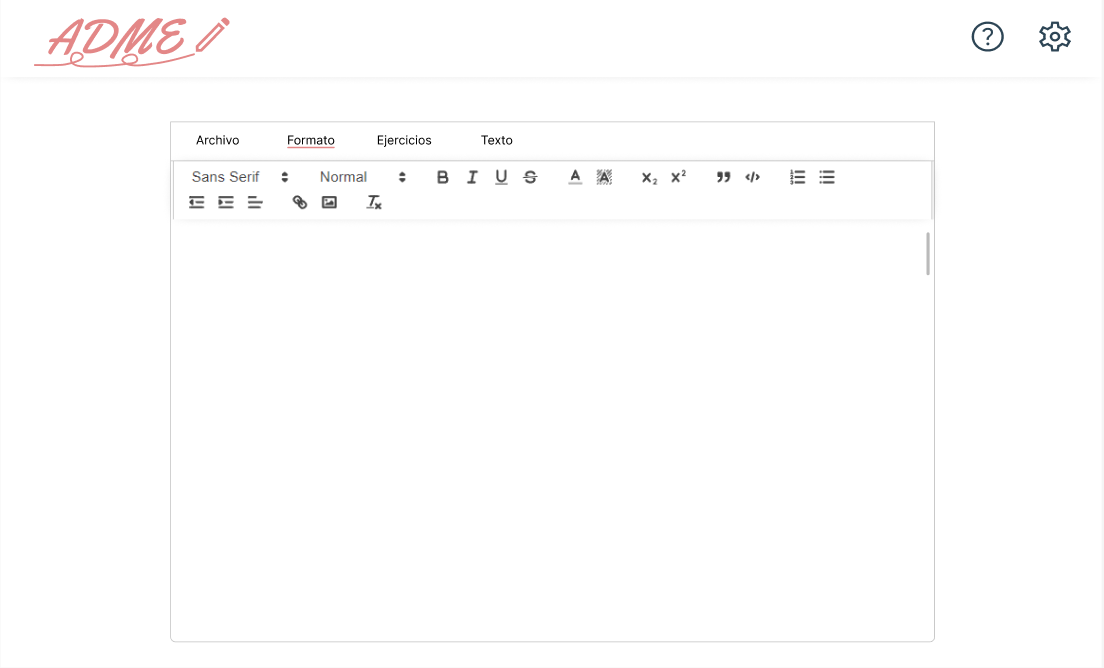
\includegraphics[width=15cm]{Diseño/Formato.PNG}
  \caption{Diseño de Formato pantalla de inicio.}
  \label{Forato}
\end{figure}


\begin{figure}[ht!]
  \centering
  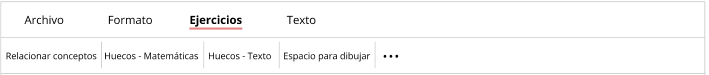
\includegraphics[width=15cm]{Diseño/Ejercicios.PNG}
  \caption{Diseño de Ejercicios pantalla de inicio.}
  \label{ejercicios}
\end{figure}


\begin{figure}[ht!]
  \centering
  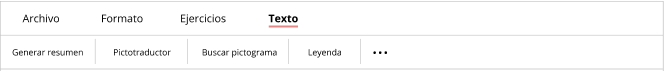
\includegraphics[width=15cm]{Diseño/Texto.PNG}
  \caption{Diseño de Texto pantalla de inicio.}
  \label{texto}
\end{figure}


\begin{figure}[ht!]
  \centering
  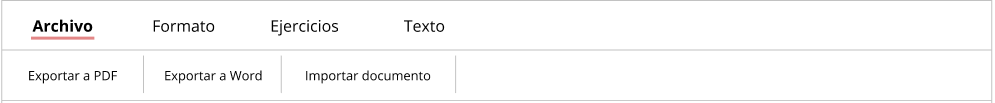
\includegraphics[width=15cm]{Diseño/Archivo.PNG}
  \caption{Diseño de Archivo pantalla de inicio.}
  \label{archivo}
\end{figure}

\subsubsection{Generar resumen}
El diseño de esta funcionalidad se muestra en la Figura \ref{resuemn} y se basa en el diseño de Álvaro Gómez, Figura \ref{fig:disenyoAlvaro03}. El usuario dispone de un panel en el que aparece el texto a resumir y el número de palabras que tendrá el resumen. Al pulsar el botón de resumir aparecerá en la parte inferior de la ventana modal una vista previa del resumen generado. El resultado de esta funcionalidad en el documento de trabajo se muestra en la Figura \ref{editable1}, en el ejercicio 3.

\begin{figure}[ht!]
  \centering
  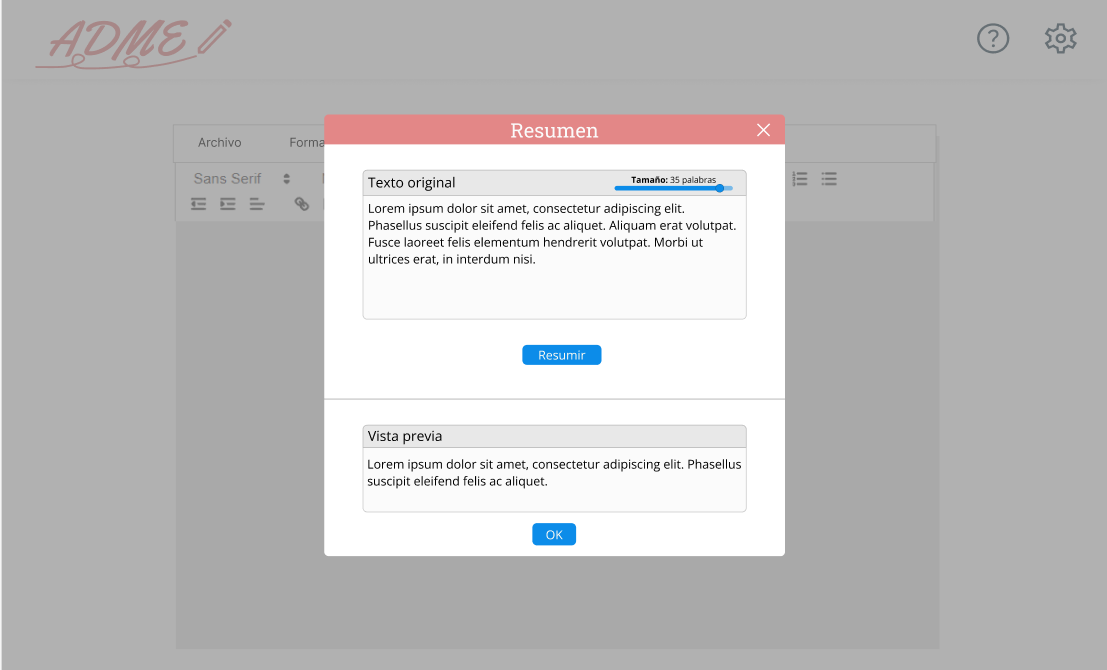
\includegraphics[width=15cm]{Diseño/Resumen.PNG}
  \caption{Diseño final generar resumen.}
  \label{resuemn}
\end{figure}

\subsubsection{Ejercicio de huecos}
El diseño de esta funcionalidad se muestra en la Figura \ref{definir_hueco}. Inicialmente habíamos pensado en que esta funcionalidad se pudiese hacer directamente sobre el documento de trabajo, pero al disponer de ventana modal y al ser complejo decidimos descartar dicha opción. En la ventana modal el usuario podrá escribir el texto. Una vez terminado le dará al botón de añadir huecos y pulsando sobre la palabra se pondrá un hueco y viceversa. Además, tiene la opción de elegir el tamaño de hueco, siendo pequeño, (5 caracteres), mediano, (12 caracteres) y grande, que es el por defecto, (23 caracteres). El resultado de esta funcionalidad en el documento de trabajo se muestra en la Figura \ref{editable3} en el ejercicio 3.

\begin{figure}[ht!]
  \centering
  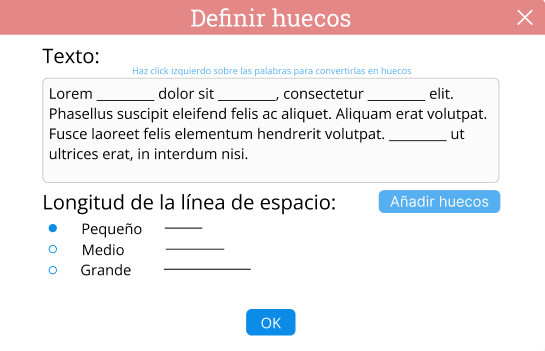
\includegraphics[width=0.7\textwidth]{Diseño/DefinirHuecos.PNG}
  \caption{Diseño final definir huecos.}
  \label{definir_hueco}
\end{figure}


\subsubsection{Sopa de letras}
El diseño de esta funcionalidad se muestra en la Figura \ref{sopaLetras}, se basa en el diseño de Alberto Rivas, (Figura \ref{Alberto16}). Inicialmente pensamos en tener dos botones, uno para añadir nuevas palabras, que se iba moviendo a la vez que se creaba una nueva palabra, y otro que se encontraba al lado de cada palabra para eliminarla, pero llegamos a la conclusión
de que era mejor que el botón de añadir palabras fuera fijo y no cambiara de posición cada vez que se añadiese una nueva palabra ya que esto le aportaría comodidad y facilidad de uso. Para ayudar al usuario a que sea más intuitivo decidimos incluir dos campos para que el usuario introduzca las filas y las columnas de la sopa de letras. También añadimos otro campo donde poner la palabra y al darle al botón de añadir la palabra se pondrá debajo de dicho campo junto a dos botones, uno de edición y otro para eliminar la palabra. Además, añadimos varias opciones para que el usuario elija cómo disponer las palabras en la sopa de letras (horizontal, vertical, diagonal y al revés). El resultado de esta funcionalidad en el documento de trabajo se muestra en la Figura \ref{editable2} en el ejercicio 5.

\begin{figure}[ht!]
  \centering
  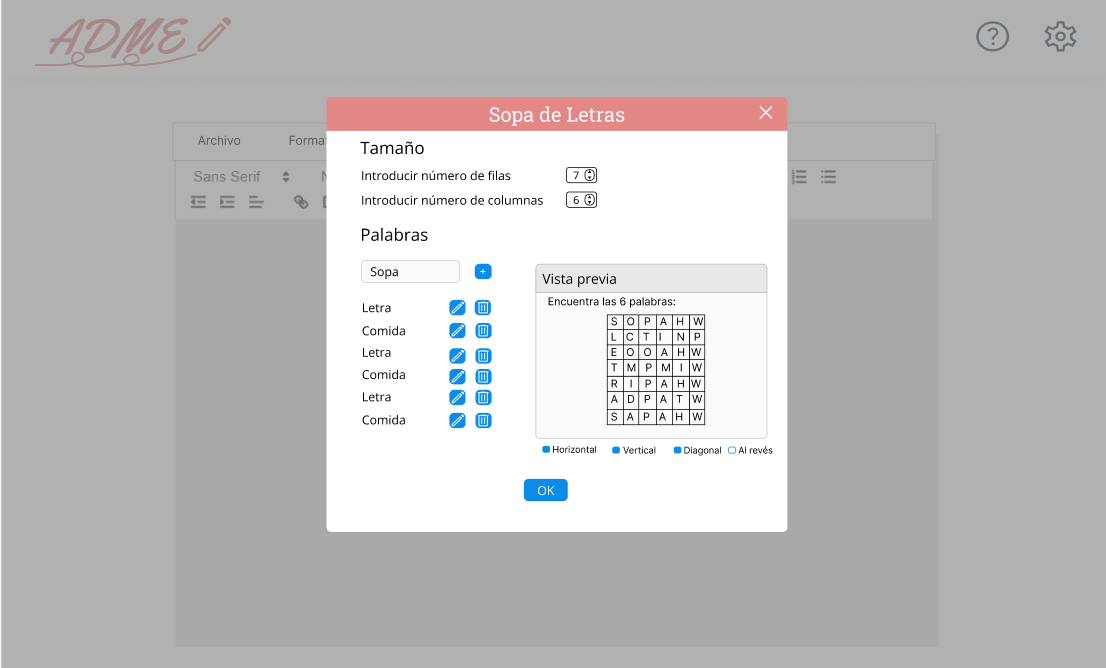
\includegraphics[width=0.7\textwidth]{Diseño/Sopa.PNG}
  \caption{Diseño final sopa de letras.}
  \label{sopaLetras}
\end{figure}

\begin{figure}[ht!]
  \centering
  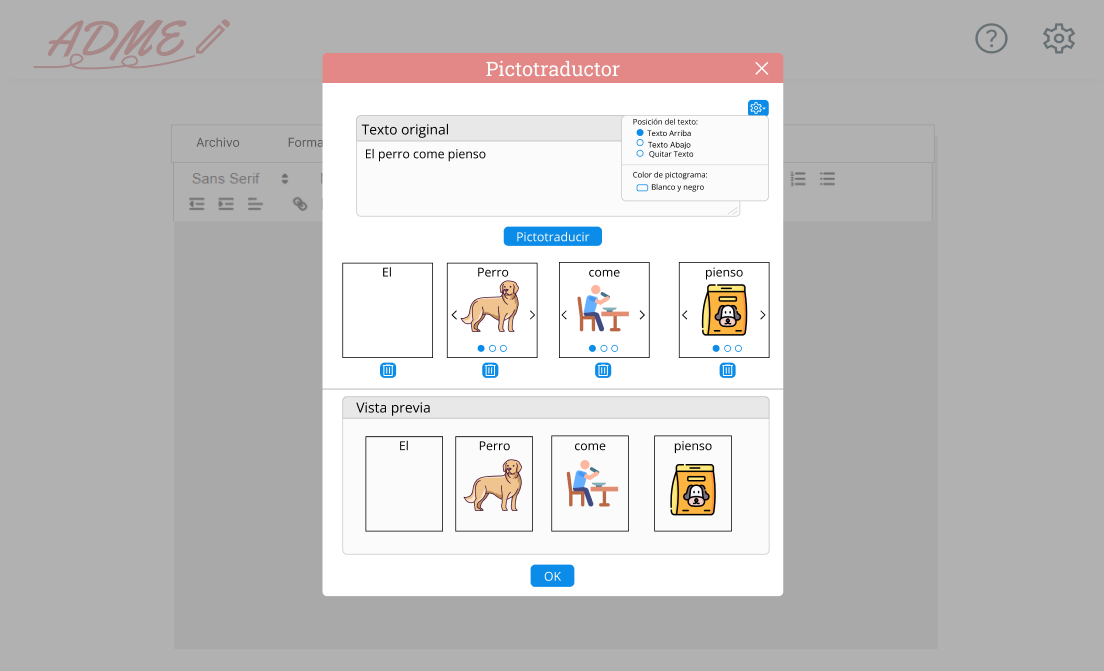
\includegraphics[width=0.7\textwidth]{Diseño/picto.PNG}
  \caption{Diseño final del pictotraductor.}
  \label{pictotraductor}
\end{figure}

\subsubsection{Pictotraductor}
El diseño de esta funcionalidad se muestra en la (Figura \ref{pictotraductor}), se basa en el diseño de Johan Salvatierra, Figura \ref{Johan7} y en la idea de Álvaro Gómez de que los pictogramas puedan cambiar en el caso de que haya varias opciones para una palabra. Inicialmente se pensó un diseño bastante simple en el que había un campo para añadir un texto y al pulsar sobre el botón de traducir a pictogramas se mostrasen los pictogramas. El problema de este diseño fue que no se tuvieron en cuenta varias opciones que necesita el usuario sobre el diseño de los pictogramas. Finalmente mantuvimos el campo de añadir el texto a traducir y el botón que te muestra los pictogramas con su respectiva palabra y añadimos un desplegable para escoger las opciones de posicionamiento de la palabra, color del pictograma y quitar la palabra asociada al pictograma. Por otra parte, cada pictograma tiene su propio botón de eliminar y unas flechas que permiten seleccionar otro de los pictogramas disponibles para la misma palabra del pictograma, en el caso de que haya varias opciones. El resultado de esta funcionalidad en el documento de trabajo se muestra en la Figura \ref{editable1} en el ejercicio 3.





\subsubsection{Ejercicio de flechas}
El diseño de esta funcionalidad se muestra en la Figura \ref{flechas} y se basa en el diseño de Dunia Namour, (Figura \ref{dunia4}). Inicialmente dábamos la opción de solo hacer dos columnas para relacionar con flechas, pero nos dimos cuenta de que el usuario debería poder elegir tantas columnas como desee. Tampoco tuvimos en cuenta que el usuario podría querer desordenar las columnas para que no tenga que pensar en el orden de las palabras. Con todo lo anterior creamos una ventana modal en la que se debe introducir el número filas y columnas, lo que genera tantas columnas vacías como haya indicado el usuario. Una vez que el usuario rellena dichas columnas tiene la opción de reordenar, la cual reordenaría cada columna. La ventana modal dispone de una vista previa en la cual se mostrará cómo quedaría el ejercicio de flechas, generándose automáticamente cada vez que el usuario realice un cambio en alguna de las columnas. El resultado de esta funcionalidad en el documento de trabajo se muestra en la Figura \ref{editable1} en el ejercicio 1.

\begin{figure}[ht!]
  \centering
  \includegraphics[width=0.7\textwidth]{Diseño/Flechas.PNG}
  \caption{Diseño final de ejercicios de fechas.}
  \label{flechas}
\end{figure}

\subsubsection{Ejercicio de desarrollo}
Partimos del diseño de AdaptaMaterialEscolar 1.0, dicho diseño no permitía al usuario cambiar el tipo de pauta ni elegir el interlineado. Todo lo mencionado anteriormente se ha añadido al nuevo diseño y también se ha incluido una vista previa que se genera automáticamente cada vez que se haga un cambio para que el usuario pueda visualizar cómo quedará el ejercicio. El diseño de esta funcionalidad se muestra en la Figura \ref{DesarrolloFinal}. El resultado de esta funcionalidad en el documento de trabajo se muestra en la Figura \ref{editable1} en el ejercicio 2.

\begin{figure}[ht!]
  \centering
  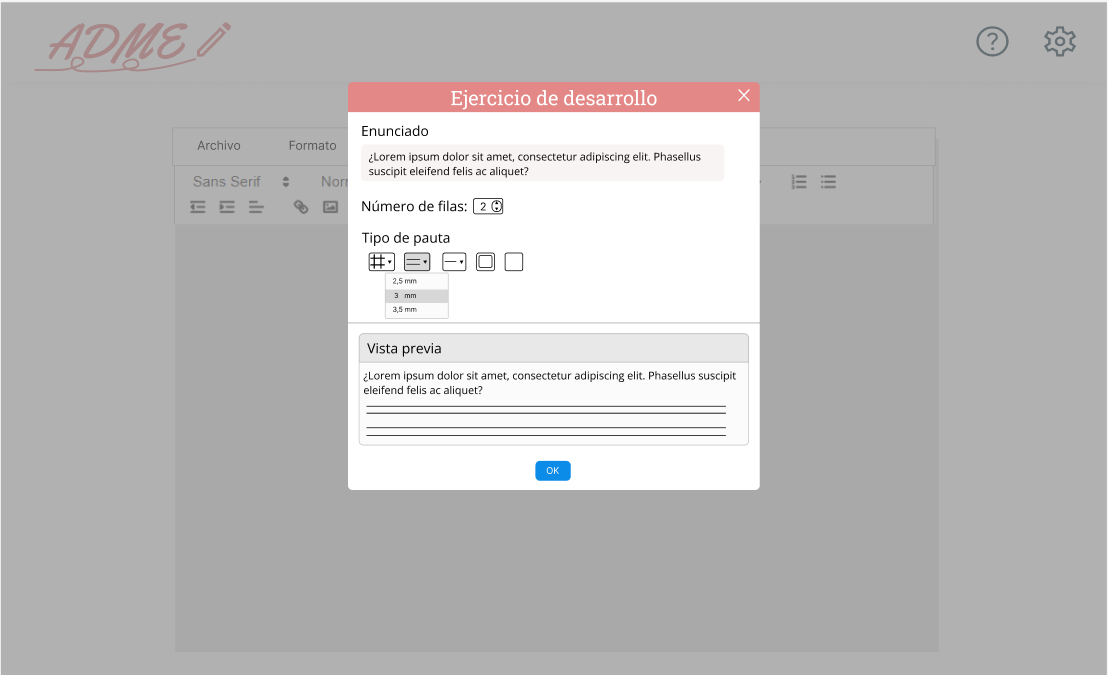
\includegraphics[width=0.7\textwidth]{Diseño/Desarollo.PNG}
  \caption{Diseño final de ejercicios de desarrollar.}
  \label{DesarrolloFinal}
\end{figure}


\begin{figure}[ht!]
  \centering
  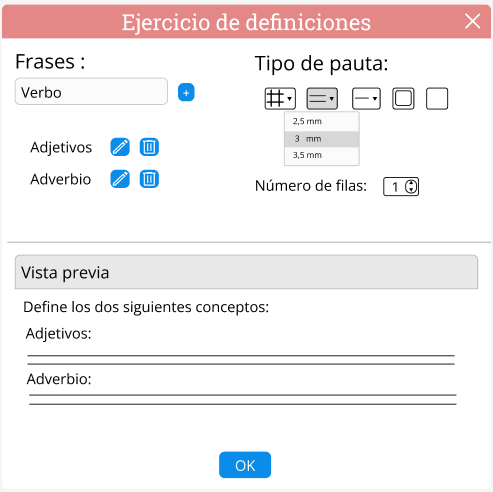
\includegraphics[width=0.7\textwidth]{Diseño/definiciones.PNG}
  \caption{Diseño final ejercicios de definiciones.}
  \label{defi}
\end{figure}

\subsubsection{Ejercicio de definiciones}
Partimos del diseño de AdaptaMaterialEscolar 1.0. Dicho diseño tenía los mismos problemas que el de ejercicios de desarrollo. El diseño final de esta funcionalidad se muestra en la Figura \ref{defi}. El resultado de esta funcionalidad en el documento de trabajo se muestra en la Figura \ref{editable2} en el ejercicio 3.


\subsubsection{Ejercicios de espacio para dibujar}
El diseño de esta funcionalidad se muestra en la Figura \ref{espaciosDibu}. En esta funcionalidad el usuario inicialmente tendrá que escribir el enunciado e indicar el espacio que desea dejar para dibujar. Además, incorpora una opción de recuadrar que hace un recuadro del tamaño indicado. El resultado de esta funcionalidad en el documento de trabajo se muestra en la Figura \ref{editable3} en el ejercicio 5.

\begin{figure}[ht!]
  \centering
  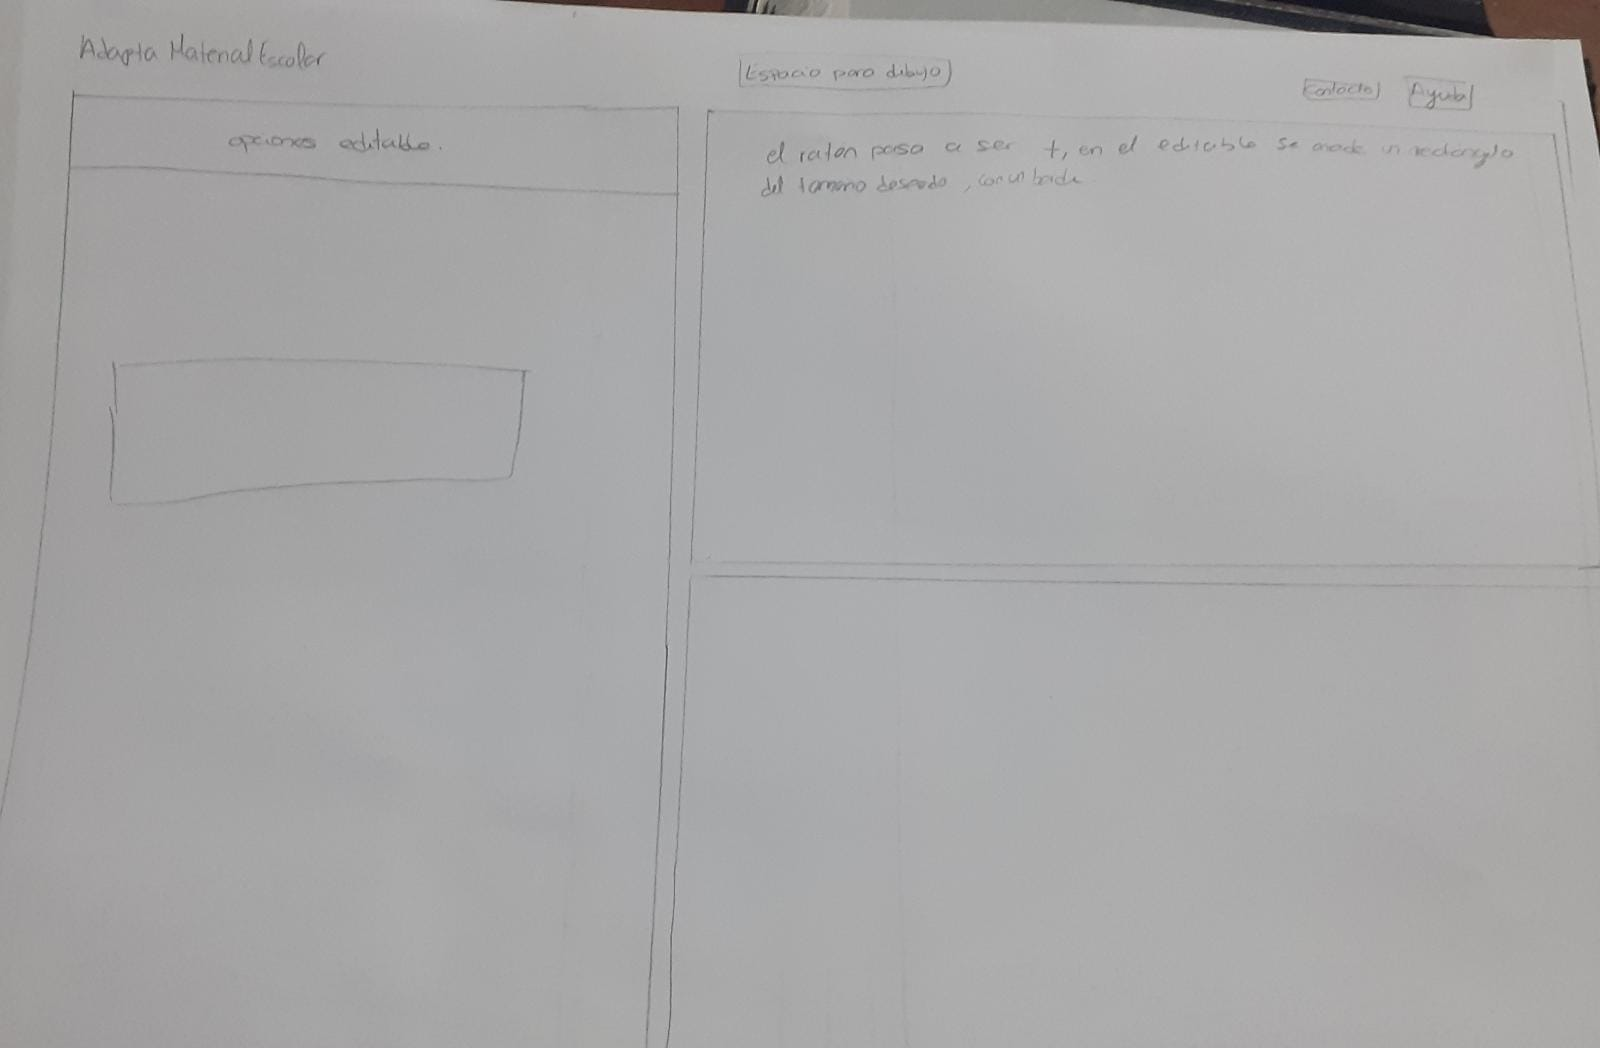
\includegraphics[width=0.7\textwidth]{Diseño/espacioDibu.PNG}
  \caption{Diseño final ejercicios espacios para dibujar.}
  \label{espaciosDibu}
\end{figure}

\subsubsection{Leyenda de colores}
El diseño final de esta funcionalidad se muestra en la Figura \ref{LeyendaColores} y para realizar esta funcionalidad no hemos basado en el diseño de todos los integrantes ya que son bastante parecidos. También hemos utilizado como referencia la funcionalidad de definir conceptos. En este caso cuando se añade un nuevo concepto también se ha de escoger un color para cada palabra. Además, se ha de incluir un título para la leyenda. La leyenda de color se situará en el documento de trabajo donde se encuentre el cursor y el usuario podrá ajustar su posicionamiento. El resultado de esta funcionalidad en el documento de trabajo se muestra en la Figura \ref{editable2} en el ejercicio 2.

\begin{figure}[ht!]
  \centering
  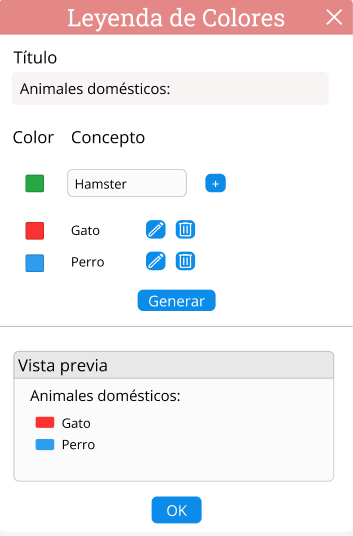
\includegraphics[width=0.7\textwidth]{Diseño/Leyenda.PNG}
  \caption{Diseño final leyenda de colores.}
  \label{LeyendaColores}
\end{figure}

\subsubsection{Ejercicio de matemáticas con huecos}
El diseño de esta funcionalidad se muestra en la Figura \ref{matesHueco} y para realizarla nos hemos basado en el diseño de Dunia Namour, Figura (\ref{dunia6}) y en la idea de Johan Salvatierra de que al pulsar la tecla \textit{espacio} se genere un hueco. Para introducir huecos en una fórmula matemática el usuario tendrá que darle a la barra espaciadora. Cuando termine de escribir la fórmula al darle al botón de \textit{OK} se introducirá en el documento de trabajo con un cuadrado vacío en cada hueco. El resultado de esta funcionalidad en el documento de trabajo se muestra en la Figura \ref{editable3} en el ejercicio 2.


\begin{figure}[ht!]
  \centering
  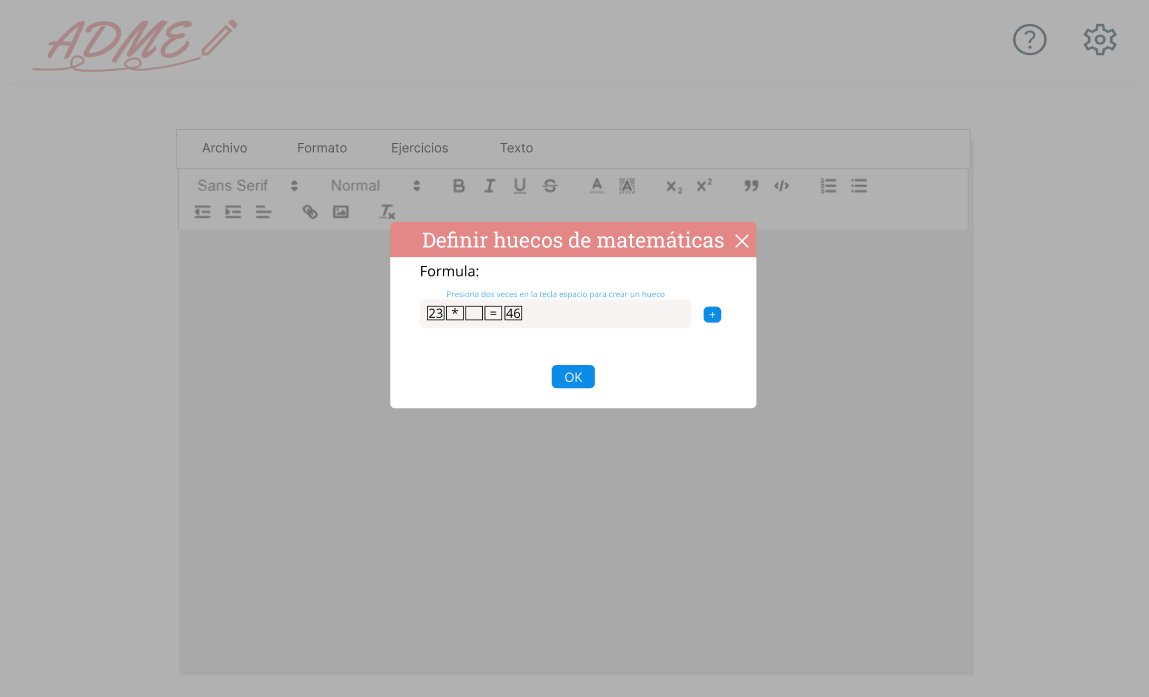
\includegraphics[width=0.7\textwidth]{Diseño/EjerMatesHuecos.PNG}
  \caption{Diseño final ejercicios de matemáticas con huecos.}
  \label{matesHueco}
\end{figure}

\subsubsection{Configuración general}
Debido a que gran parte de las funcionalidades tienen varias opciones hemos decidido crear una página de configuración para poder definir los ajustes por defecto. En esta página hay una configuración general por cada tipo de funcionalidad. El diseño de la configuración se muestra en la Figura \ref{configu}. Esta página surgió durante el brainstorming con las tutoras por la necesidad de tener ajustes por defecto.

\begin{figure}[ht!]
  \centering
  \includegraphics[width=15cm]{Diseño/configuracion.PNG}
  \caption{Diseño final de la configuración general.}
  \label{configu}
\end{figure}





\begin{figure}[ht!]
  \centering
  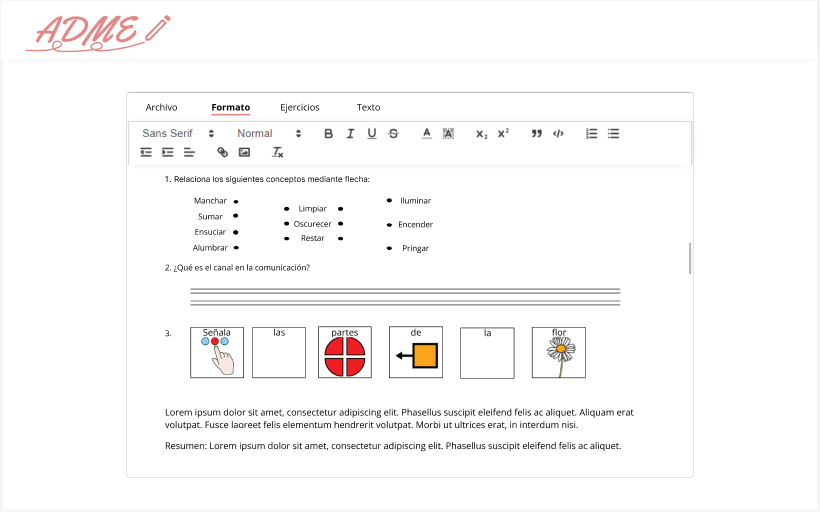
\includegraphics[width=15cm]{Diseño/Editable1.PNG}
  \caption{Resultado de las funcionalidades en el documento de trabajo.}
  \label{editable1}
\end{figure}


\begin{figure}[ht!]
  \centering
  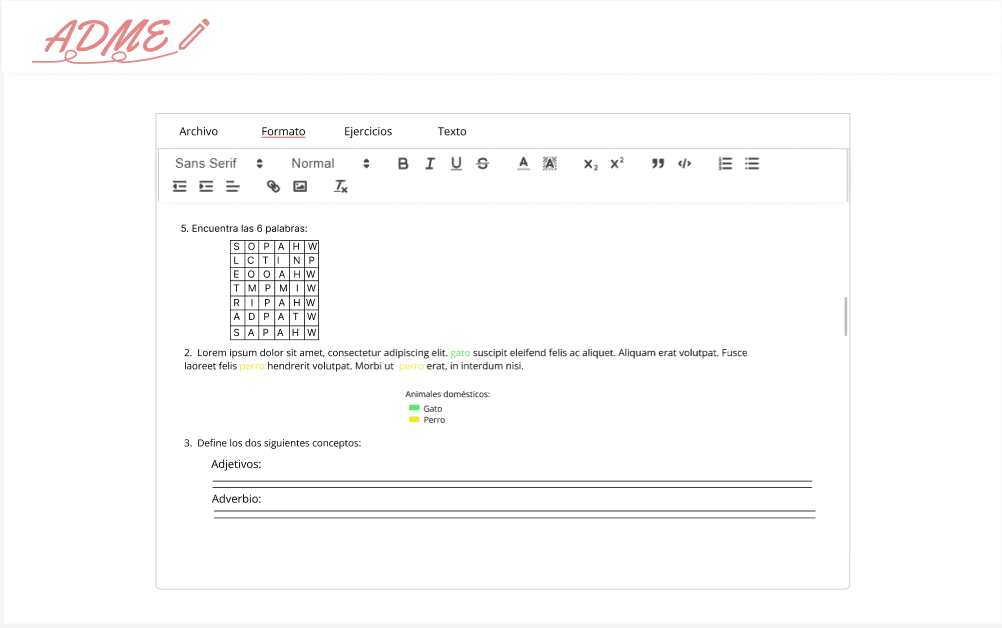
\includegraphics[width=15cm]{Diseño/editable2.PNG}
  \caption{Resultado de las funcionalidades en el documento de trabajo.}
  \label{editable2}
\end{figure}

\begin{figure}[ht!]
  \centering
  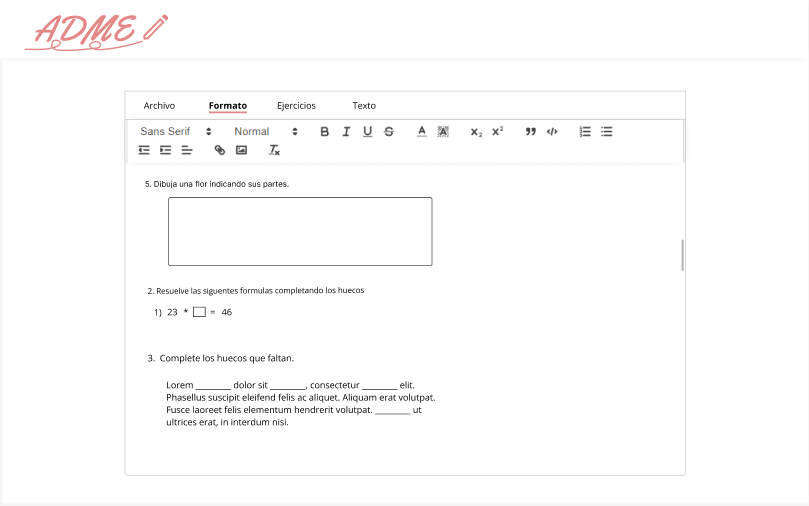
\includegraphics[width=15cm]{Diseño/Editable3.PNG}
  \caption{Resultado de las funcionalidades en el documento de trabajo.}
  \label{editable3}
\end{figure}

\section{Implementación}
% TODO: Introduccion
\subsection{Arquitectura}
En este TFG hemos decidido usar Slate, una biblioteca de JavaScript que se utiliza para construir editores de texto enriquecido. Lo hemos combinado con React lo que nos permite crear una aplicación basada en componentes que a largo plazo será más escalable. Ambas herramientas se apoyan en el patrón \textit{Composite}\footnote{\url{https://refactoring.guru/es/design-patterns/composite}} el cual permite generar un componente complejo mediante la anidación de componentes simples. Dicho patrón se encuentra integrado en Slate lo que nos facilita la configuración de este. En cuanto a la estructura interna de React ayuda a implementarlo, por nuestra parte lo hemos empleado para el diseño de los modales. Por otro lado, también hemos usado el patrón creacional \textit{Factory}\footnote{\url{https://refactoring.guru/es/design-patterns/factory-method}} que nos permite crear objetos sin tener que conocer los detalles de su creación, lo hemos usado para la creación de los modales y de las distintas barras de herramientas que se encuentran en el editor.

En cuanto a cómo se encuentran conectados Slate y React cabe mencionar que hemos creado un conjunto de funciones que hacen de intermediario entre los modales y el editor.

\begin{figure}[ht!]
  \begin{subfigure}{\textwidth}
    \centering
    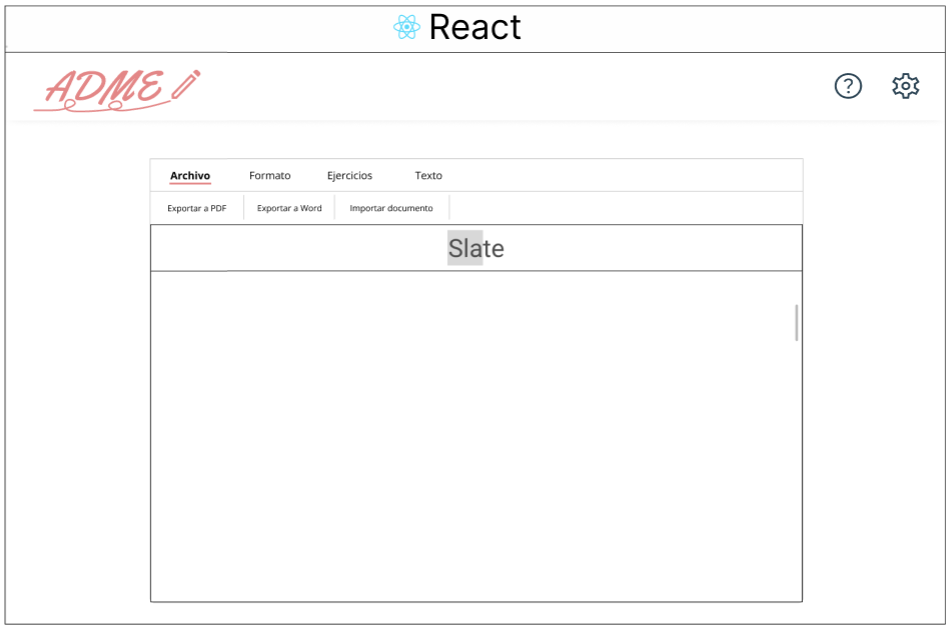
\includegraphics[width=0.7\textwidth]{Arquitectura/ArquitecturaPaginaInicio.png}
    \caption{Visión general de la página de inicio}
    \label{fig:arquitecturageneral1}
  \end{subfigure}

  \begin{subfigure}{\textwidth}
    \centering
    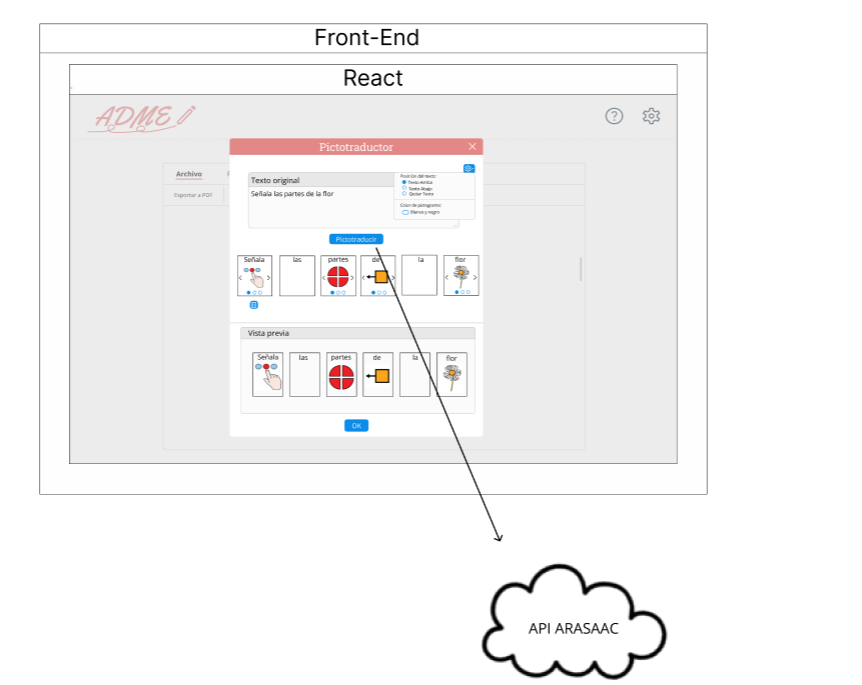
\includegraphics[width=0.7\textwidth]{Arquitectura/ArquitecturaPictoTraductor.png}
    \caption{Visión general de funcionalidad con conexión a API}
    \label{fig:arquitecturageneral2}
  \end{subfigure}
  \caption{Visión general de AdaptaMaterialEscolar 2.0}
  \label{fig:arquitecturageneral}
\end{figure}

\subsection{Funcionalidades}
A continuación se explican los detalles de implentación de las distintas funcionalidades que hemos rediseñado o creado de cero.
% TODO: Terminar introduccion

Para la explicación de las funcionalidades se pensó en realizar diagramas para facilitar la comprensión, pero tras debatirlo con las tutoras de este TFG y con Antonio Navarro Martín (profesor de Ingeniería y Modelado de Software), se llegó a la conclusión de que no hay aproximaciones para modelar React y JavaScript. Se comentó la posibilad de extender diagramas UML, utilizando la tesis de Humberto Cortés y Antonio Navarro\footnote{\url{https://www.worldscientific.com/doi/abs/10.1142/S0218194017500486}}, para poder modelar React y JavaScript, pero eso podría ser un TFG en sí mismo.

\chapter{Conclusiones y Trabajo Futuro}
\label{cap:conclusiones}

En la Sección \ref{sec:conclusiones} se explicará las conclusiones a las que se han llegado tras realizar el proyecto y en la Sección \ref{sec:TrabajoFuturo} se describirá las posibles mejoras que se podrían llevar a cabo en la aplicación.

\section{Conclusiones}
\label{sec:conclusiones}
En este Trabajo de Fin de Grado (TFG), se planteó como objetivo principal el desarrollo de una aplicación web que facilite la adaptación curricular no significativa para los docentes. Para lograr dicho objetivo, se investigaron los distintos tipos de adaptaciones y herramientas disponibles. La aplicación fue diseñada con el propósito de ofrecer una amplia variedad de adaptaciones. Para ello, se inició un proceso de rediseño de AdaptaMaterialEscolar 1.0, a través de una iteración competitiva con todos los miembros del equipo, siguiendo una metodología de Diseño Centrado en el Usuario (DCU). Además, se realizaron cambios en la arquitectura del proyecto y las tecnologías utilizadas. Entre los cambios destacados, se migró de una arquitectura \textit{serverless} a una arquitectura cliente-servidor. También se decidió no utilizar Redux ni Sass y se empezó a utilizar Tailwind CSS. Asimismo, debido a que la licencia de CKEditor que se utilizaba en AdaptaMaterialEscolar 1.0 expiró y no fue posible renovarla, se implementó el editor de texto utilizando Slate. Se tuvo que implementar completamente los requisitos mínimos del editor que se solicitaron para AdaptaMaterialEscolar 1.0, ya que Slate no ofrece funcionalidades básicas de editor, sino utilidades para implementarlas. En el desarrollo de la aplicación se incluyeron la mayoría de los ejercicios y herramientas propuestos, como la funcionalidad de nuevo archivo, exportar a PDF, relacionar conceptos, ejercicios de matemáticas con huecos, ejercicio con espacio para dibujar, leyenda de colores, generar resumen y pictotraductor. Las funcionalidades implementadas en AdaptaMaterialEscolar 1.0 tuvieron que ser creadas desde cero debido a los cambios en la arquitectura y el rediseño, así como a ciertos cambios en los requisitos. Una vez desarrollada la aplicación, se alojó en un servidor de Oracle para llevar a cabo una evaluación con usuarios. Como resultado de dicha evaluación, se recopilaron datos sobre la usabilidad y utilidad de la aplicación.

Además, otro objetivo del TFG fue aplicar y ampliar los conocimientos adquiridos durante la carrera. Las asignaturas más influyentes para el desarrollo del TFG fueron:

\begin{itemize}
    \item \textbf{Gestión de proyectos Software}: Se centra en la planificación, organización, seguimiento y control de todos los aspectos de un proyecto de software, desde la concepción hasta la entrega final del producto. En esta asignatura hemos aprendido cómo administrar los recursos y el tiempo para garantizar que los proyectos se completen dentro de los plazos establecidos. También hemos aprendido la importancia de establecer objetivos claros, crear un plan de proyecto sólido y hacer un seguimiento regular del progreso para garantizar que el proyecto esté en camino.
    \item \textbf{Aplicaciones Web}: Enseña a cómo diseñar y desarrollar aplicaciones web eficientes y escalables. Además, cubre una amplia variedad de tecnologías, desde el diseño y la creación de interfaces de usuario hasta la gestión de bases de datos y la seguridad de aplicaciones. En concreto hemos utilizado los conocimientos adquiridos sobre \textit{HTML}, \textit{CSS}, \textit{JavaScript} y \textit{Node.js}.
    \item \textbf{Ingeniería del Software, Modelado de Software}: Las asignaturas de Ingeniería de Software y Modelado de Software son importantes para el desarrollo de software de alta calidad. La primera se enfoca en los principios, prácticas y técnicas necesarias para crear software eficiente y funcional. La segunda se enfoca en crear modelos precisos y detallados antes de la implementación para reducir errores y permitir una implementación más rápida y efectiva. En ambas asignaturas se cubren técnicas y habilidades esenciales para el proceso de desarrollo de software. En concreto hemos aplicado los conocimientos adquiridos sobre la gestión de errores y los patrones de diseño.
    \item \textbf{Estructura de Datos}: La comprensión de las estructuras de datos y las técnicas de manipulación de datos son esenciales para el desarrollo de software de alta calidad y eficiente. Esta asignatura proporciona una base sólida para construir soluciones de software más efectivas y escalables en el futuro. En concreto hemos aplicado los conocimientos adquiridos para entender mejor la estructura de Slate.
    \item \textbf{Ética, legislación y profesión}: Se centra sobre los aspectos éticos y legales de la ingeniería de software, como la privacidad de los datos, la propiedad intelectual, la responsabilidad social y profesional, y la seguridad del software. También se enseñan las leyes y regulaciones relevantes, como la Ley de Protección de Datos Personales y la Ley de Propiedad Intelectual.
    \item \textbf{Administración de Sistemas y Redes}: Se centra en la administración de sistemas operativos, incluyendo la instalación, configuración y mantenimiento de servidores y clientes. También se enseña la administración de redes, incluyendo la configuración de routers, switches y firewalls, la gestión de direcciones IP y el monitoreo del tráfico de la red. En concreto hemos aplicado los conocimientos adquiridos para montar el servidor en el que se ha alojado la aplicación.
\end{itemize}

Durante el desarrollo de la aplicación AdaptaMaterialEscolar, hemos adquirido nuevos conocimientos sobre el uso de tecnologías, como React, ampliamente utilizada en el mundo laboral. Además, hemos aprendido y aplicado eficazmente Tailwind CSS y Slate, herramientas que han contribuido a una experiencia de desarrollo más eficiente y flexible. También hemos con usuarios finales, identificando y satisfaciendo sus necesidades.

\section{Trabajo Futuro}
\label{sec:TrabajoFuturo}
Después de desarrollar el proyecto y cumplir con la mayoría de los requisitos fijados al principio del trabajo, es inevitable que queden algunas tareas pendientes para posible trabajo futuro.

Desde el punto de vista de los requisitos, ya en la Sección \ref{cap:requisitos} se comentó las funcionalidades descartadas por falta de información. En concreto estos requisitos son:
\begin{itemize}
    \item Añadir imágenes buscando una palabra.
    \item Sustituir una palabra por una imagen.
    \item Crear una herramienta de recorte de imágenes para el texto original.
    \item Crear tablas que organicen el temario y/o las actividades, seleccionando contenido.
    \item Crear esquemas.
    \item Ejercicios de completar los espacios en blanco en tablas y esquemas.
\end{itemize}

Desde la perspectiva de los requisitos, se han dado requisitos que se han postergado por la prioridad establecida de los requisitos. Específicamente, estos requisitos son:
\begin{itemize}
    \item Importar a Word: no lo hemos realizado porque requeriría cambiar el comportamiento de los elementos tratados por Slate. Condideramos que era muy complejo y había otras funcionalidades con igual o mayor prioridad.
    \item Exportar a Word: No se ha realizado porque su implementación es similar a importar a Word.
    \item Sección de ayuda: Aunque consideramos que es importante, no se ha realizado ya que hemos priorizado la calidad del editor y de las adaptaciones, además de la cantidad de adaptaciones.
    \item Configuración general: Para implementar la configuración se necesitaría utilizar cookies de navegador para guardar la información aumentando considerablemente la complejidad de la aplicación. Para cada adaptación habría que guardar información sobre todas sus posibles opciones de configuración. Consideramos que nos iba a llevar mucho tiempo conseguir que funcionara correctamente y preferimos implementar más adaptaciones y mejorar el funcionamiento tanto del editor como de las adaptaciones.
\end{itemize}

La evaluación de la aplicación ha generado nuevas ideas y requisitos para realizar mejoras, basadas en las peticiones y propuestas recibidas por los docentes evaluadores. Estas son algunas de las sugerencias:

\begin{itemize}
    \item Capacidad de reorganizar los ejercicios en el documento de trabajo: Se requiere la opción de mover los ejercicios dentro del documento de manera intuitiva y sencilla.
    \item Funcionalidad de deshacer y rehacer en el documento de trabajo: Es necesario implementar una función que permita al usuario deshacer y rehacer acciones previas, proporcionando una forma de restaurar cambios no deseados.
    \item Añadir botón de ``ayuda'' para realizar las adaptaciones: Se sugiere añadir un botón de ayuda en todas las ventanas modales de las adaptaciones, el cual proporcionará información sobre el uso de la funcionalidad en cuestión.
\end{itemize}
\begin{otherlanguage}{english}
  \chapter{Conclusions and Future Work}
\label{cap:conclusions}


In Section \ref{sec:conclusions}, the conclusions reached after completing the project are explained, and in Section \ref{sec:FutureWork}, possible improvements that could be implemented in the application are described.

\section{Conclusions}
\label{sec:conclusions}
The main objective of this Degree Final Project (TFG) was to develop a web application that facilitates non-significant curricular adaptation for teachers. To achieve this general objective, we set several specific objectives. Next we will see if we have achieved each of these specific objectives:

\begin{itemize}
    \item Analyze AdaptaMaterial 1.0 to identify the requirements that were not covered and the improvements that could be made. As shown in Section \ref{cap:requisitos}, we conducted this analysis and identified the requirements for our application.
    \item Redesign the application. This objective has also been achieved as we completely redesigned the interface, as presented in Section \ref{disenyoDeLaAplicacion}. Additionally, we refactored the application: we transitioned from a serverless architecture to a client-server architecture, migrated from class-based components to functional components, updated the React router to the latest available version, decided not to use Redux or Sass, and started using Tailwind CSS. Lastly, due to the expiration of the CKEditor license used in AdaptaMaterialEscolar 1.0 and the impossibility of renewing it, we implemented the text editor using Slate.
    \item Improvement of existing features and addition of new features. Regarding the development and definitions features present in the previous version (AdaptaMaterialEscolar 1.0), we have incorporated the ability to choose the type of ruling (double, single, grid), and we have also added the option to select a school font type. Additionally, we have introduced several new features, including: generating a summary, exporting the working document to Word and PDF, importing to Word, pictotranslator, content matching exercises, color legend, exercises with space for drawing, and mathematical formulas. All of these features have been implemented except for the import and export to Word.
    \item We conducted an evaluation with end users who provided feedback through a Google Form survey. The survey consisted of three parts: creating an exam model, preparing adapted notes, and a general evaluation of the application. Each task was accompanied by an explanation and an image, followed by three evaluation questions. After the first two parts, a ten-question questionnaire on ease of use was conducted. Open-ended responses were also requested to gather opinions about the tool.

    The results obtained demonstrate that we have exceeded expectations, achieving a notable score of 78.5 on the System Usability Scale (SUS). Furthermore, analyzing Figure \ref{fig:graficaComparativaEjerciciosApuntes}, we can observe that users were more satisfied and comfortable using the features for generating exercises compared to the features for creating notes.
\end{itemize}



In addition, at the beginning of the Degree Final Project (TFG), we set ourselves two academic objectives that we have also achieved:
\begin{itemize}
    \item Apply the knowledge acquired during our degree to this project.
    \begin{itemize}
        \item \textbf{Software Project Management}: This subject focuses on the planning, organization, monitoring, and control of all aspects of a software project, from conception to the final product delivery. In this course, we have learned how to manage resources and time to ensure that projects are completed within established deadlines. Specifically, in this project, we have used the Kanban methodology, which we learned in Software Project Management. This allowed us to create a solid project plan and regularly track progress to ensure the project stays on track.
        \item \textbf{Web Applications}: Teaches how to design and develop efficient and scalable web applications. It covers a wide variety of technologies, from user interface design and creation to database management and application security. Specifically, in this project, we have utilized the knowledge acquired in HTML, CSS, JavaScript, and Node.js.
        \item \textbf{Software Engineering, Software Modeling}: Software Engineering and Software Modeling subjects are important for the development of high-quality software. The former focuses on the principles, practices, and techniques necessary to create efficient and functional software, while the latter focuses on creating accurate and detailed models before implementation to reduce errors and enable faster and more effective implementation. Both subjects cover essential techniques and skills for the software development process. Specifically, in this project, we have applied the acquired knowledge regarding error management and design patterns.
        \item \textbf{Data Structures}: Understanding data structures and data manipulation techniques is essential for the development of high-quality and efficient software. This subject provides a solid foundation for building more effective and scalable software solutions in the future. Specifically, we have applied the acquired knowledge to better understand the structure of Slate.
        \item \textbf{Ethics, Legislation, and Profession}: This subject focuses on the ethical and legal aspects of software engineering, such as data privacy, intellectual property, social and professional responsibility, and software security. It also covers relevant laws and regulations, such as the Personal Data Protection Law and the Intellectual Property Law. Specifically, we have applied the acquired knowledge to understand how to use and manage third-party code, as well as managing the license for our project.
        \item \textbf{Systems and Networks Administration}: This subject focuses on the administration of operating systems, including server and client installation, configuration, and maintenance. It also covers network administration, including router, switch, and firewall configuration, IP address management, and network traffic monitoring. Specifically, we have applied the acquired knowledge to set up the server where the application has been hosted.
    \end{itemize}

    \item Acquire new knowledge.

    During the development of the AdaptaMaterialEscolar 2.0 application, we have acquired new knowledge about the use of technologies such as React, widely used in the professional world. Additionally, we have effectively learned and applied Tailwind CSS and Slate, tools that have contributed to a more efficient and flexible development experience. We have also worked with end-users, identifying and meeting their needs.
\end{itemize}


\section{Future Work}
\label{sec:FutureWork}
After developing the project and accomplishing most of the objectives set initially, it is inevitable that some tasks remain pending for possible future work.

From a requirements perspective, in Section \ref{cap:requisitos}, we already discussed the functionalities that were discarded due to lack of information.

\begin{itemize}
    \item Add image search by keyword.
    \item Substitute a word with an image.
    \item Create an image cropping tool for the original text.
    \item Create tables to organize the syllabus and/or activities, selecting content.
    \item Create diagrams.
    \item Exercises to fill in the blanks in tables and diagrams.
\end{itemize}

On the other hand, there have been certain requirements that have not been carried out due to the priority established among them. Specifically, these requirements are:

\begin{itemize}
    \item Import to Word: We have not implemented this because it would require changing the behavior of the elements handled by Slate. We considered it too complex, and there were other functionalities with equal or higher priority.
    \item Export to Word: The implementation of this functionality has not been carried out due to its similarity to the import to Word function. Just like in the case of importing to Word, we considered that this implementation would be too complex, and there were other functionalities with equal or higher priority.
    \item Help section: Although we consider it important, it has not been implemented as we prioritized the quality of the editor and the adaptations, as well as the quantity of adaptations.
    \item General configuration: To implement the general configuration, it would be necessary to use browser cookies to store the information, significantly increasing the complexity of the application. For each adaptation, information about all its possible configuration options would need to be stored. Additionally, it would involve a significant amount of data management since each adaptation can have multiple configuration options, requiring the storage and management of a large amount of related data. Therefore, we believed it would take a long time to make it work correctly, and we preferred to implement more adaptations and improve the functionality of both the editor and the adaptations.
\end{itemize}

The evaluation of the application has generated improvement ideas and new requirements:

\begin{itemize}
    \item Ability to rearrange exercises: The evaluators missed being able to change the order of the exercises.
    \item Allow undo and redo actions for all operations to make the user feel in control of the application and explore it without fear of making mistakes. This new functionality would also enable the user to easily recover from errors.
    \item Add help to all the features.
    \item Allow the selection of specific words to appear in the summary.
    \item Improve wording regarding punctuation and connectors to provide cohesion in the text.
    \item When translating text into pictograms, articles should be omitted as they are complex to represent through drawings.
    \item Improve exercise editing in the working document.
    \item Allow the generation of non-numbered exercises.
    \item Enhance advanced text editing features.
    \item Automatically assign colors to text based on selected categories in the color legend.
    \item Improve the functionality of math exercises because evaluators found it confusing.
\end{itemize}
\end{otherlanguage}
\chapter{Trabajo Individual}
\label{cap:TrabajoIndividual}

En este capítulo se habla del trabajo que ha realizado cada miembro del equipo en el proyecto.

\section{Álvaro Gómez Sittima}
Durante el desarrollo de este TFG, he colaborado en la creación de la aplicación y la redacción de la memoria. A continuación se exponen las distintas actividades que he realizado a lo largo de este TFG, tanto de manera individual como en grupo, para alcanzar los objetivos establecidos. Las actividades se han clasificado en las siguientes categorías: estudio de la cuestión, captura de requisitos, diseño de la aplicación, implementación, evaluación, metodología, QA y memoria.

En cuanto al estudio de la cuestión, investigué sobre las distintas herramientas existentes que ayudan a realizar adaptaciones curriculares no significativas. Esta investigación ayudó a clarificar el objetivo del TFG, además de aportar ideas para el diseño e implementación de ciertas funcionalidades similares a las herramientas estudiadas. También me informé sobre alternativas a CKEditor, proponiendo Quill.js, aunque finalmente nos decantamos por la opción que propuso Johan (Slate) ya que se integraba mejor con React. Otras herramientas y frameworks que investigué y propuse para utilizar en la implementación son: Tailwind CSS, Flowbite, Prettier y ESLint.

En cuanto a la captura de requisitos, se definieron, en grupo, las distintas agrupaciones de requisitos (formato, ejercicios y auxiliar) y se decidió que requisitos se implementarían y cuáles no, ya fuese porque ya estaban implementados o por falta de información.

Con respecto al diseño de la aplicación, todos los miembros del equipo realizamos diseños individuales para la iteración competitiva. Estos diseños se utilizaron como boceto inicial y tras compararlos en una reunión con las tutoras del TFG, se definió el estilo y diseño general de la aplicación. Los diseños individuales los hice en papel y se encuentran en el Apéndice \ref{ape:disenyoAlvaro}. Tras la reunión, colaboré con Johan en la realización de los diseños en Figma y, en grupo, diseñamos el logo de ADME.

En cuanto a la implementación, he integrado Tailwind CSS como framework CSS para la aplicación. Además, he realizado la refactorización y limpieza del código para facilitar la escalabilidad y la implementación de nuevas funcionalidades en el futuro. Asimismo, he creado distintos componentes reutilizables para facilitar la creación de nuevas ventanas modales, como por ejemplo el propio componente de la ventana modal, botones o la vista previa. En cuanto a las funcionalidades, me he encargado de desarrollar las funcionalidades de crear ejercicios de completar huecos, sopa de letras, generar resúmenes y pictotraductor. En cuanto al editor, he implementado algunas de las funcionalidades básicas, como cambiar el tipo de fuente, el tamaño de letra, el color de la fuente, resaltar el texto con un color de fondo y distintos formatos básicos de fuente (subrayado, tachado y cursiva). En colaboración con el grupo, hemos desarrollado la estructura principal de la aplicación, incluyendo la página de inicio, la barra de navegación y el editor. También hemos desarrollado la función de buscar pictograma.

Con respecto al Quality Assurance (QA), he sido el responsable de proponer distintos planes de prueba, herramientas y técnicas para poder garantizar la calidad del código. En cuanto a la ejecución del plan de pruebas, me he encargado de arreglar los bugs de las funcionalidades de crear ejercicios de completar huecos, sopa de letras, generar resúmenes y pictotraductor. También he probado las funcionalidades de verdadero/falso y ejercicios de matemáticas con huecos. Los casos de prueba y procedimientos de la funcionalidad de verdadero/falso se realizaron en grupo (Sección \ref{planPruebas:v/f}), mientras que los de la funcionalidad de ejercicios de matemáticas con huecos los realicé individualmente (Sección \ref{planPruebas:mates}). Además, he integrado herramientas destinadas a mejorar la calidad del código, tales como Prettier, con el fin de definir un estilo común en todo el proyecto, y ESLINT, para llevar a cabo análisis estáticos del código.

En cuanto a la evaluación, Dunia se encargó principalmente de esta parte. Yo aporté una segunda opinión y algunas ideas para la realización de las plantillas y el formulario.

En cuanto a la metodología, colaboré en la definición del tablero Kanban y las políticas explícitas.

Con respecto a la memoria, he contribuido individualmente en la redacción de diferentes secciones de la memoria, tales como la Sección \ref{sec:herramientasexistentes}, en la cual se realiza una comparativa con otras aplicaciones similares a AdaptaMaterialEscolar, la Sección \ref{sec:qa} donde se explican las técnicas y el plan de pruebas aplicados en el proyecto para asegurar la calidad de la aplicación, la Sección \ref{sec:tailwind}, en la cual se explica el framework Tailwind CSS, la Sección \ref{sec:prettier}, en la cual se explica la herramienta Prettier para dar formato al código y la Sección \ref{sec:eslint}, en la cual se explica la herramienta de linting ESLint. Además, he redactado la implementación de las funcionalidades que he desarrollado: completar huecos (Sección \ref{sec:impcompletarhuecos}), sopa de letras (Sección \ref{sec:impsopaletras}), generar resumen (Sección \ref{sec:impresumen}) y pictotraductor (Sección \ref{sec:imppictotraductor}). También, he explicado mis diseños para la iteración competitiva, Sección \ref{sec:iterAlvaro}. Junto a mis compañeros, he participado en la definición de los objetivos (Sección \ref{cap:objetivos}), la definición de requisitos (Sección \ref{cap:requisitos}), el diseño final de la aplicación (Sección \ref{subsec:DisenyoFinal}), la visualización del flujo Kanban (Sección \ref{sec:flujoTrabajo}), las políticas explícitas Kanban (Sección \ref{sec:politicas}), la arquitectura de la aplicación (Sección \ref{sub:Arquitectura}), la implementación de la funcionalidad de buscar pictogramas (Sección \ref{sec:impbuscarpicto}) y las conclusiones y trabajo futuro (Capítulo \ref{cap:conclusiones}).

\section{Dunia Namour Doughani}
A lo largo de este TFG he desempeñado varias tareas tanto individualmente como con los integrantes de este equipo para lograr cada objetivo propuesto. En cuanto a las actividades, pueden ser clasificadas en varias categorías: estudio de la cuestión, captura de requisitos, diseño de la aplicación, implementación, evaluación, metodología, QA y memoria.
\begin{itemize}
    \item Estudio de la cuestión: En esta categoría se presenta la investigación realizada sobre la adaptación curricular, que es el tema principal abordado. Individualmente redacté la Sección \ref{cap:adaptacion}, la cual proporciona una explicación sobre la adaptación curricular y sus diferentes tipos.
    \item Captura de requisitos: En esta categoría se presenta las tareas relacionadas con el proceso de identificar y documentar las necesidades de los usuarios. En la Sección \ref{cap:requisitos} definimos y clasificamos todos juntos los requisitos.
    \item Diseño de la aplicación: En esta categoría se presenta las tareas relacionadas con el proceso de crear y definir la estructura, apariencia y funcionalidad de una aplicación. La primera tarea que realicé fue la creación de los diseños para la iteración competitiva, los cuales se describen en la Sección \ref{sec:duniaIter}. También creé en Figma cómo se verían los ejercicios en el documento de trabajo. Como equipo diseñamos el logo de la aplicación en Figma.
    \item Implementación: En esta categoría se presenta las tareas relacionadas con la construcción y puesta en marcha de la aplicación. Individualmente implementé la funcionalidad de verdadero y falso (Sección \ref{sec:funcioVF}) y de leyenda de colores (Sección \ref{sec:leyendaColores}). También llevé a cabo una refactorización de la funcionalidad de verdadero y falso para sustituir el CSS por la librería de diseño Tailwind. En cuento al trabajo en equipo, aporté en el desarrollo de la funcionalidad de búsqueda de pictogramas y en la pantalla de inicio.
    \item Evaluación: En esta categoría se presenta las tareas relacionadas con el proceso de medir y analizar el desempeño de la aplicación. Realicé la plantilla de examen, los apuntes y el formulario de evaluación para que los usuarios finales puedan valorar AdaptaMaterialEscolar 2.0.
    \item Metodología: En esta categoría se expone las tareas relacionadas con el conjunto de prácticas y técnicas utilizadas para planificar y llevar a cabo un proyecto. Colaboré en la redacción de la sección del tablero Kanban en la Sección \ref{sec:flujoTrabajo} y en la definición de las políticas explícitas en la Sección \ref{sec:politicas}.
    \item QA (Quality Assurance): En esta categoría se expone las tareas relacionadas con el conjunto de procesos, técnicas y actividades enfocadas en garantizar la calidad de la aplicación. Para ello realicé de forma individual la corrección de los errores relacionados con la funcionalidad de leyenda de colores y la funcionalidad de verdadero y falso. También dediqué tiempo a probar y desarrollar un plan de pruebas detallado para las funcionalidades de sopa de letras y buscar pictograma. Además, llevé a cabo el test de múltiples funcionalidades, incluyendo las de relacionar conceptos, pictotraductor, espacios para dibujar y de exportar a PDF. Finalmente, realicé un segundo test en las funcionalidades de desarrollo y definiciones, resumen y huecos de matemáticas. A cerca del trabajo en equipo, colaboré en la redacción del plan de pruebas para la funcionalidad de verdadero y falso y brindé apoyo a Álvaro en la refactorización del código.
    \item Memoria: En esta categoría se describen las tareas implicadas en la redacción de los diferentes capítulos del TFG. Individualmente me encargué de redactar la Sección \ref{cap:estructura}, donde se hace una breve descripción de cada capítulo escrito en dicha memoria. También expliqué la herramienta React en el capítulo sobre herramientas empleadas, la Sección \ref{sec:React}. Además, incluí las imágenes de las funcionalidades diseñadas en Figma. Por último, incluí el plan de pruebas, escrito en un documento aparte, en la memoria en el Anexo \ref{ape:pruebas}. En relación al trabajo conjunto participé en la redacción de los objetivos del proyecto en la Sección \ref{cap:objetivos}. También desarrollamos el diseño final de cada funcionalidad en la Sección \ref{subsec:DisenyoFinal} y la arquitectura en la Sección \ref{sub:Arquitectura}. Asimismo, redactamos la implementación de la funcionalidad de búsqueda de pictograma en la Sección \ref{sec:impbuscarpicto} y los capítulos de introducción en inglés (Capítulo \ref{cap:introduction}), evaluación (Capítulo \ref{cap:evaluacion}) y trabajo futuro (Capítulo \ref{cap:conclusiones}).
\end{itemize}


\section{Alberto Alejandro Rivas Fernandez}
Durante este TFG he participado tanto en el desarrollo de la aplicación como en la redacción de la memoria. A continuación, se explican más en detalle mis aportaciones individuales y de trabajo en grupo.

En cuanto a la captura de requisitos, tuvimos que realizarla en grupo para decidir cuáles eran las funcionalidades que íbamos a incluir en la versión final de la aplicación basándonos en las necesidades de los usuarios. Esta se encuentra explicada en detalle en la Sección \ref{cap:requisitos}.

Para realizar el diseño de la aplicación, todos los integrantes del grupo hicieron un diseño individual para luego compararlo con el de los demás. Debido a esto, tuve que realizar el diseño de la página principal de la aplicación y de cada una de las funcionalidades que decidimos implementar al hacer la captura de requisitos. Estos fueron hechos en Figma ya que quería mostrar exactamente cómo se vería en la aplicación final, incluyendo colores, fuente de letra, etc.

Al principio del proyecto, uno de los desafíos que enfrentamos fue la necesidad de implementar la funcionalidad de exportar documentos en formato Word y PDF. CKEditor tiene un plugin que nos permite hacer esto, pero necesitábamos una licencia de pago para poder utilizarlo. Me puse en contacto con el equipo de CKEditor con el fin de obtener una licencia gratuita. Sin embargo, después de varios intentos y comunicaciones con el equipo, no pudimos obtenerla, por lo que tuvimos que buscar otra librería para implementar el editor de texto.

Una de las librerías que decidimos probar fue Quill.js. En nuestra aplicación usamos modales para cada funcionalidad, entonces hice la prueba de implementar modales utilizando esta librería y utilizando también Redux. Sin embargo, decidimos no usar Redux ya que encontramos una forma más sencilla de implementar los modales en Quill. Luego decidimos no usar Quill.js ya que encontramos otra librería llamada Slate.js que se adapta mejor a nuestras necesidades.

Una vez que decidimos que librería utilizar, empezamos a implementar las funcionalidades. La primera funcionalidad que implementé fue la de ejercicios de desarrollo. Para implementar esta funcionalidad tuve que aprender a utilizar Slate para poder insertar el ejercicio en nuestro editor de texto.

Los estilos de la funcionalidad anterior los había realizado con CSS. Sin embargo, decidimos usar Tailwind, el cual es un framework de CSS. Debido a esto, tuve que aprender a usar este framework y refactorizar el código para implementar los estilos con Tailwind en vez de CSS.

Un compañero hizo el \textit{testing} de la funcionalidad que yo había implementado y encontró algunos errores que tuve que arreglar. Por ejemplo, se podía insertar el ejercicio en el editor sin enunciado, el modal no se reseteaba al cerrarlo, etc.

Después de esto trabajé en implementar la funcionalidad de crear ejercicios de matemática con huecos. Al igual que antes, un compañero realizó el \textit{testing} de la funcionalidad de crear ejercicios de matemática y encontró una serie de errores que tuve que arreglar. Además de eso, se nos ocurrió añadir funciones nuevas, como poder agregar varias fórmulas al mismo tiempo, por ejemplo, por lo que también realicé esos cambios.

Por último, también realicé la implementación de la funcionalidad de espacios para dibujar.

En cuanto al trabajo en grupo en el código, desarrollamos la funcionalidad de buscar pictograma en conjunto para luego usarla como referencia al implementar el resto de las funcionalidades individualmente, realizamos el plan de pruebas de la funcionalidad de ejercicios de verdadero y falso, y también ayudamos a Álvaro con la refactorización del código, con el objetivo de hacerlo más reutilizable.

En cuanto a las metodologías utilizadas para el desarrollo en equipo de este TFG, en el capítulo de metodología (Capítulo \ref{cap:metodologia}), redactamos juntos la sección de visualizar el flujo de trabajo (Sección \ref{sec:flujoTrabajo}), en la que explicamos cómo usaremos el tablero Kanban en nuestro proyecto y también escribimos la sección de políticas explícitas (Sección \ref{sec:politicas}), en la que enumeramos las reglas que debemos seguir al usar este tablero.

En cuanto al control de calidad (QA), realicé el \textit{testing} de las funcionalidades de ejercicio de definiciones y leyenda de colores para garantizar su correcto funcionamiento. También escribí su plan de pruebas correspondiente. Para hacer el \textit{testing} de las funcionalidades, estuve realizando varias pruebas con diferentes inputs con el fin de encontrar algún error o algún caso de uso que no funcionase correctamente.

Con respecto a la memoria, me encargué de redactar la sección \ref{cap:adaptaMaterial} que habla sobre la primera versión de AdaptaMaterialEscolar. Además expliqué la implementación de las funcionalidades de ejercicios de desarrollo y de ejercicios de matemática con huecos en las secciones \ref{sec:impdesarrollo} y \ref{sec:impmatematica}.

También redacté la explicación detallada de cada uno de los diseños individuales en la sección \ref{sec:albertoIter} de la memoria para explicar las decisiones de diseño tomadas.

En cuanto al trabajo en grupo en la memoria, hemos redactado la Sección \ref{cap:objetivos}, en la que explicamos los objetivos de este TFG. También hemos traducido al inglés todo el capítulo de introducción (Capítulo \ref{cap:introduction}). En el capítulo de AdaptaMaterialEscolar 2.0 (Capítulo \ref{cap:AdaptaMaterialEscolar2.0}), redactamos la sección en la que explicamos los requisitos de la aplicación (Sección \ref{cap:requisitos}), el diseño final (Sección \ref{subsec:DisenyoFinal}) y la arquitectura (Sección \ref{sub:Arquitectura}), en la sección de funcionalidades, en la que explicamos la implementación de cada una, escribimos la implementación de buscar pictograma (Sección \ref{sec:impbuscarpicto}) en grupo para después hacer las demás individualmente. Por último, diseñamos el logo de la aplicación entre todos.


\section{Johan Sebastian Salvatierra Gutierrez}
Durante el desarrollo de este TFG, he llevado a cabo diversas tareas, tanto de forma individual como en equipo, con el fin de alcanzar los objetivos propuestos. Estas tareas pueden ser clasificadas en diferentes categorías, tales como: estudio de la cuestión, captura de requisitos, diseño de la aplicación, implementación, evaluación, metodología, QA y memoria. A continuación, se detallará cada una de estas categorías.

En la categoría de captura de requisitos (Sección \ref{cap:requisitos}), que se refiere al proceso de identificar y documentar las necesidades de los usuarios, participé en la definición y clasificación conjunta de los requisitos del proyecto.

En la categoría de diseño de la aplicación, se presentan las tareas relacionadas con el proceso de crear y definir la estructura, apariencia y funcionalidad de una aplicación. La primera tarea que realicé fue la creación de los diseños para la iteración competitiva, los cuales se describen en la Sección \ref{sec:johanDisenyo}. Añadí un anexo explicando el diseño que propuse. Junto a Álvaro, realicé los diseños finales en Figma. Como equipo, diseñamos el logo de la aplicación también en Figma y las ideas de cómo se vería el diseño final.

En la implementación, realicé una investigación exhaustiva para encontrar un editor de texto que pudiera satisfacer los requisitos del proyecto y después de evaluar varias opciones, seleccioné Slate como el framework adecuado. Posteriormente, realicé un prototipo con Slate integrado con React para comprobar su viabilidad y propuse su uso para el proyecto. Trabajé en la creación de ejercicios de definiciones (Sección \ref{sec:ejercicioDefiniciones}) y creé pautas en formato SVG que pudieran reutilizarse en diferentes ejercicios. También creé el nodo Tablas con todas las funciones necesarias para gestionarlos y modifiqué su formato para que otras funciones pudieran utilizarlo. Además, desarrollé la función para crear ejercicios de relacionar conceptos (Sección \ref{sec:ejercicioRelacionarConceptos}) y cree la forma para que los ejercicios tuvieran una edición dinámica a través del modal que los creo. Para ello, abstraje los diferentes nodos de los ejercicios en uno solo que permitiera la edición independientemente del ejercicio, y creé la numeración automática de los ejercicios a partir de este nodo. Asimismo, desarrollé parte de la funcionalidad básica del editor, como las formas de listar y los tipos de alineación. Investigué cómo hacer que las imágenes e iconos se comportaran de la forma deseada y dediqué tiempo a investigar la forma en que todos los elementos pudieran exportarse a PDF con el menor impacto posible. También me encargué de configurar y lanzar el host para la aplicación. En cuanto al trabajo en equipo, colaboré en el desarrollo de la funcionalidad de búsqueda de pictogramas y en la pantalla de inicio, y contribuí con Álvaro en la abstracción del código, lo que nos permitió desarrollar una base de código más modular y fácil de mantener.

En la categoría de metodologías, se abordan las tareas relacionadas con el conjunto de prácticas y técnicas empleadas para planificar y llevar a cabo un proyecto. Expliqué las clases de servicio en la Sección \ref{claseDeServicio} que empleamos para el tablero Kanban. Colaboré en la redacción de la sección del tablero Kanban en la Sección \ref{sec:flujoTrabajo} y en la definición de las políticas explícitas en la Sección \ref{sec:politicas}.

En la categoría de QA (Aseguramiento de calidad), se incluyen las tareas relacionadas con el conjunto de procesos, técnicas y actividades enfocadas en garantizar la calidad de la aplicación. En mi rol individual, me encargué de corregir los errores relacionados con la funcionalidad de definiciones, relacionar conceptos y exportar PDF. Asimismo, realicé pruebas de la función ``generar resumen'' y ``desarrollo''. En cuanto al trabajo en equipo, colaboré en la redacción del plan de pruebas para la funcionalidad de verdadero y falso, y brindé apoyo a Álvaro en la refactorización del código.

En la categoría de memoria, se describen las tareas implicadas en la redacción de los diferentes capítulos del TFG. He redactado diversas secciones, incluyendo la Sección \ref{cap:motivacio}, donde se presenta la motivación detrás del proyecto, y la Sección \ref{Editor}, donde se explica detalladamente los tipos de nodos y su integración con la aplicación. También he descrito el editor utilizado en esta sección, el cual se ha integrado con éxito en la aplicación. Además, he incluido una explicación detallada de la herramienta Slate en el capítulo de herramientas empleadas, en la Sección \ref{sec:Slate}. En cuanto a mi contribución en equipo, he colaborado en la redacción de los objetivos del proyecto en la Sección \ref{cap:objetivos}. También hemos desarrollado conjuntamente el diseño final de cada funcionalidad en la Sección \ref{subsec:DisenyoFinal} y la arquitectura en la Sección \ref{sub:Arquitectura}. Por último, he participado en la descripción de la implementación de la funcionalidad de búsqueda de pictograma en la Sección \ref{sec:impbuscarpicto} y en la redacción del capítulo de introducción en inglés en el Capítulo \ref{cap:introduction}.




% Apéndices
\appendix
\chapter{Diseños individuales para la iteración competitiva de Álvaro Gómez Sittima}
\label{ape:disenyoAlvaro}
En este apéndice se muestran los diseños individuales realizados por Álvaro Gómez Sittima para la iteración competitiva. En la Figura \ref{fig:disenyoAlvaro01} se muestra el diseño de la pantalla de inicio, tanto con un archivo PDF como sin él. En la Figura \ref{fig:disenyoAlvaro02} se presenta la funcionalidad de generar resumen. En la Figura \ref{fig:disenyoAlvaro03} se muestra el diseño de la funcionalidad de pictotraductor. En la Figura \ref{fig:disenyoAlvaro04} se muestra el diseño del ejercicio de completar huecos. En la Figura \ref{fig:disenyoAlvaro05} se presenta la funcionalidad de buscar pictogramas. Finalmente, en la Figura \ref{fig:disenyoAlvaro06} se muestra el diseño de la funcionalidad de crear ejercicios de definiciones.

\begin{figure}[ht!]
  \centering

  \begin{subfigure}{\textwidth}
    \centering
    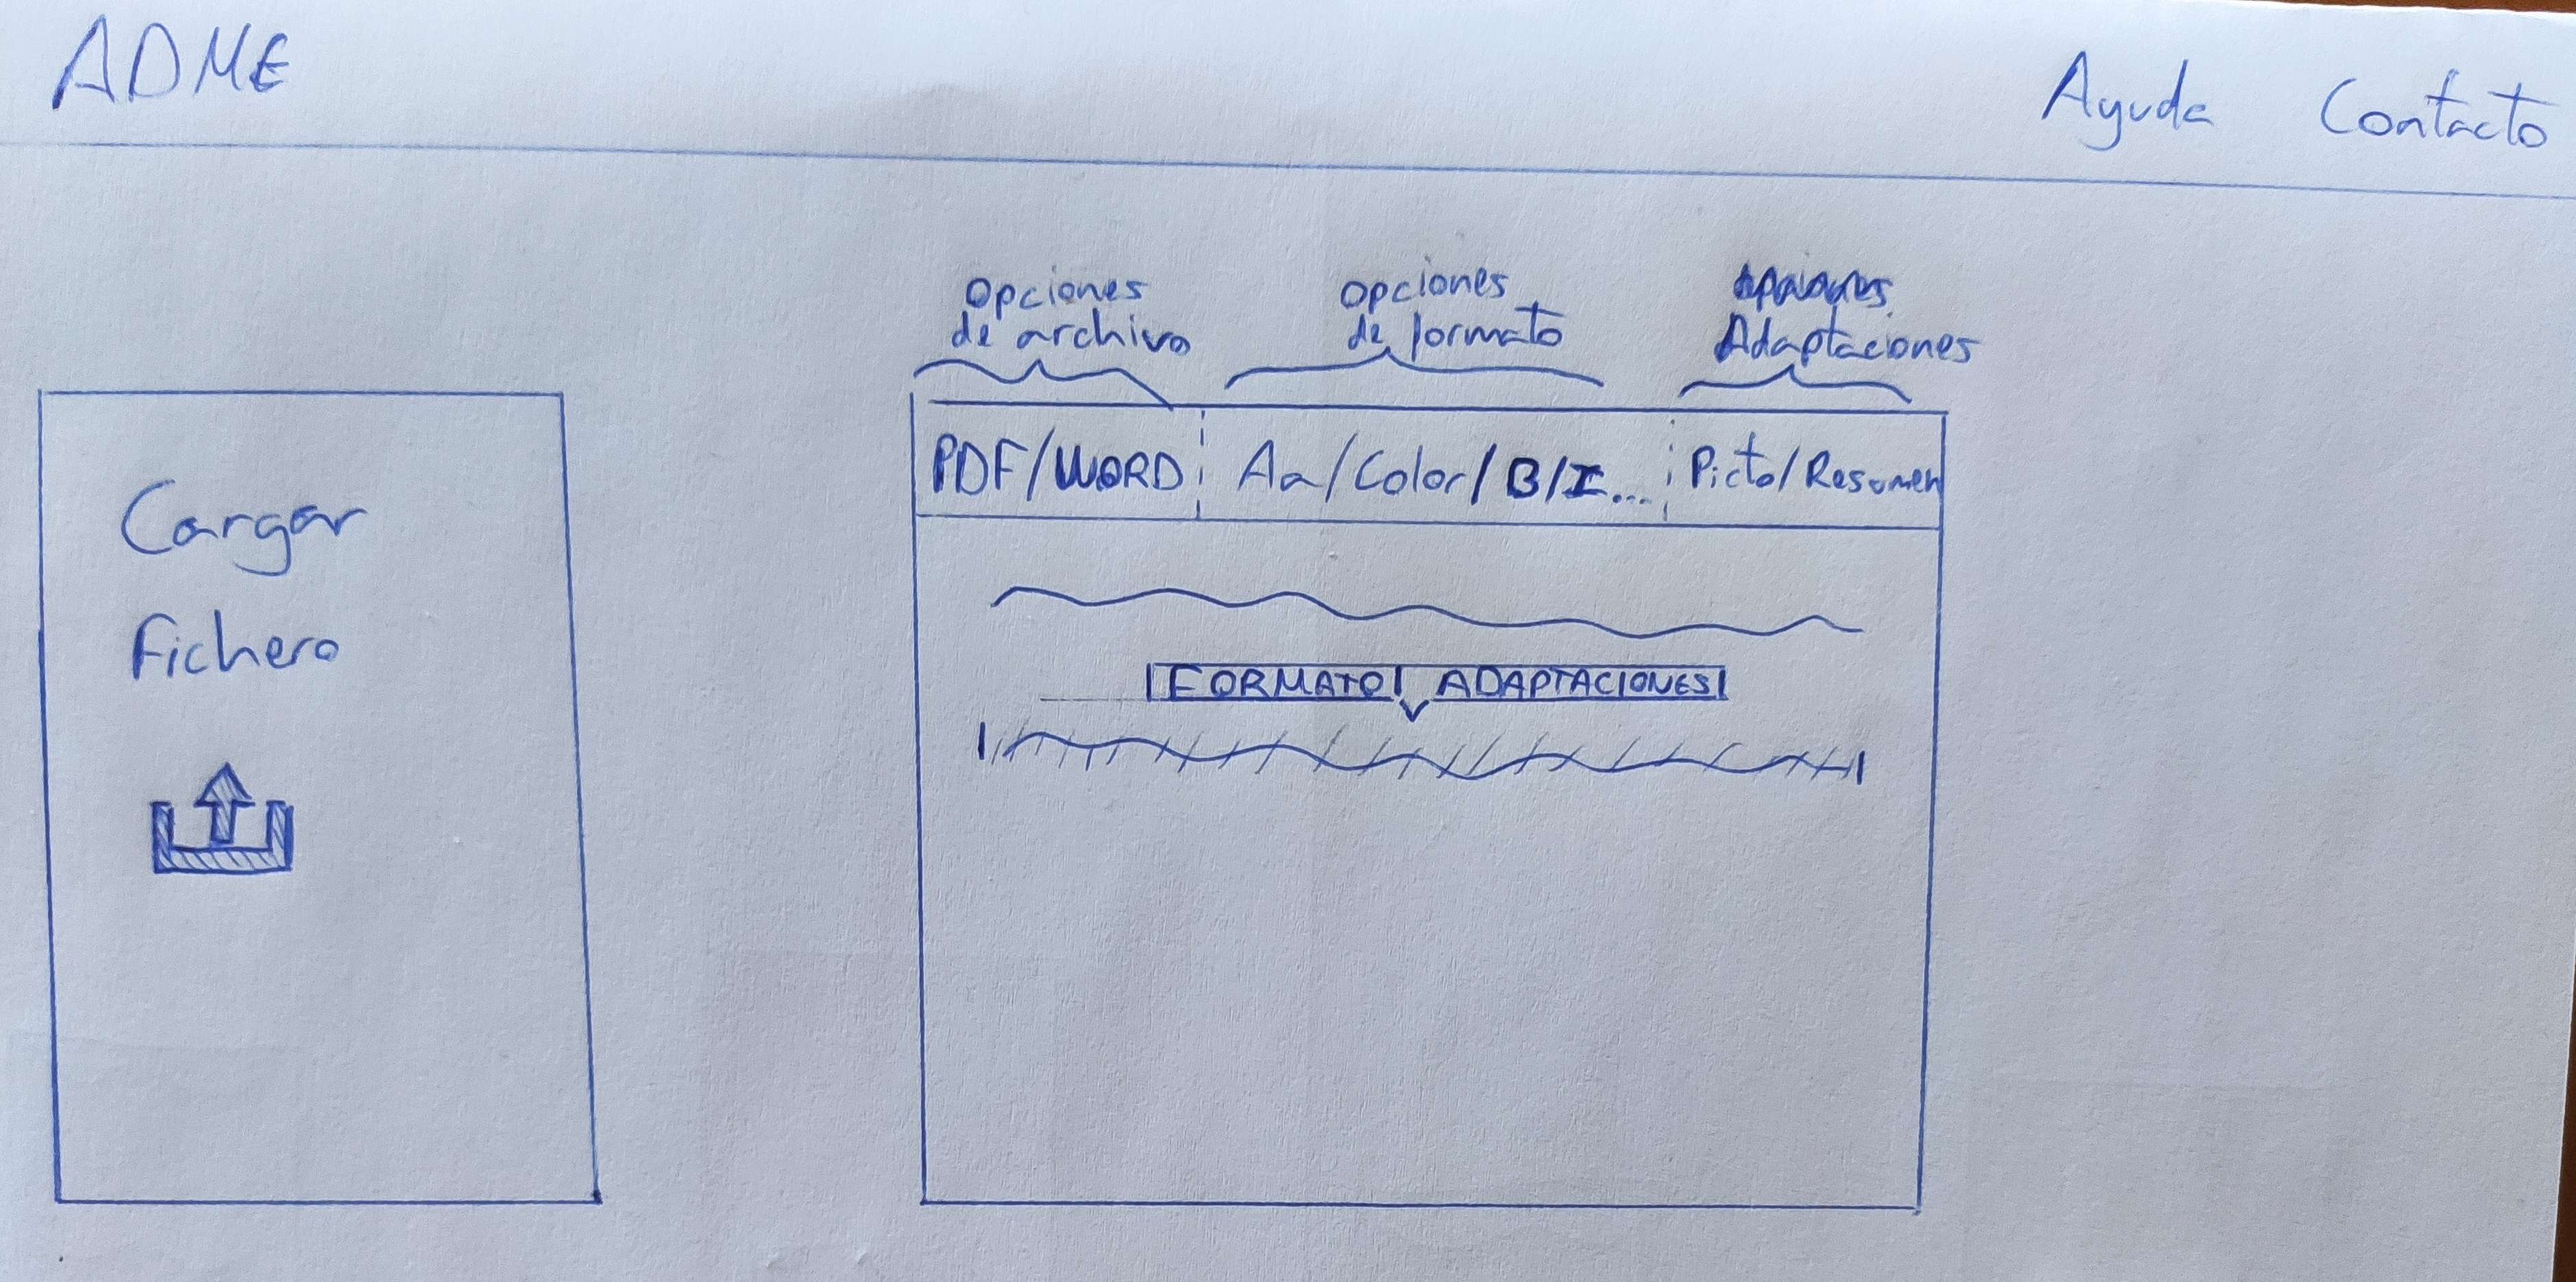
\includegraphics[width=0.7\textwidth]{Diseño/Alvaro/Alvaro01.jpg}
    \caption{Página de inicio sin PDF.}
    \label{fig:disenyoAlvaro01a}
  \end{subfigure}

  \begin{subfigure}{\textwidth}
    \centering
    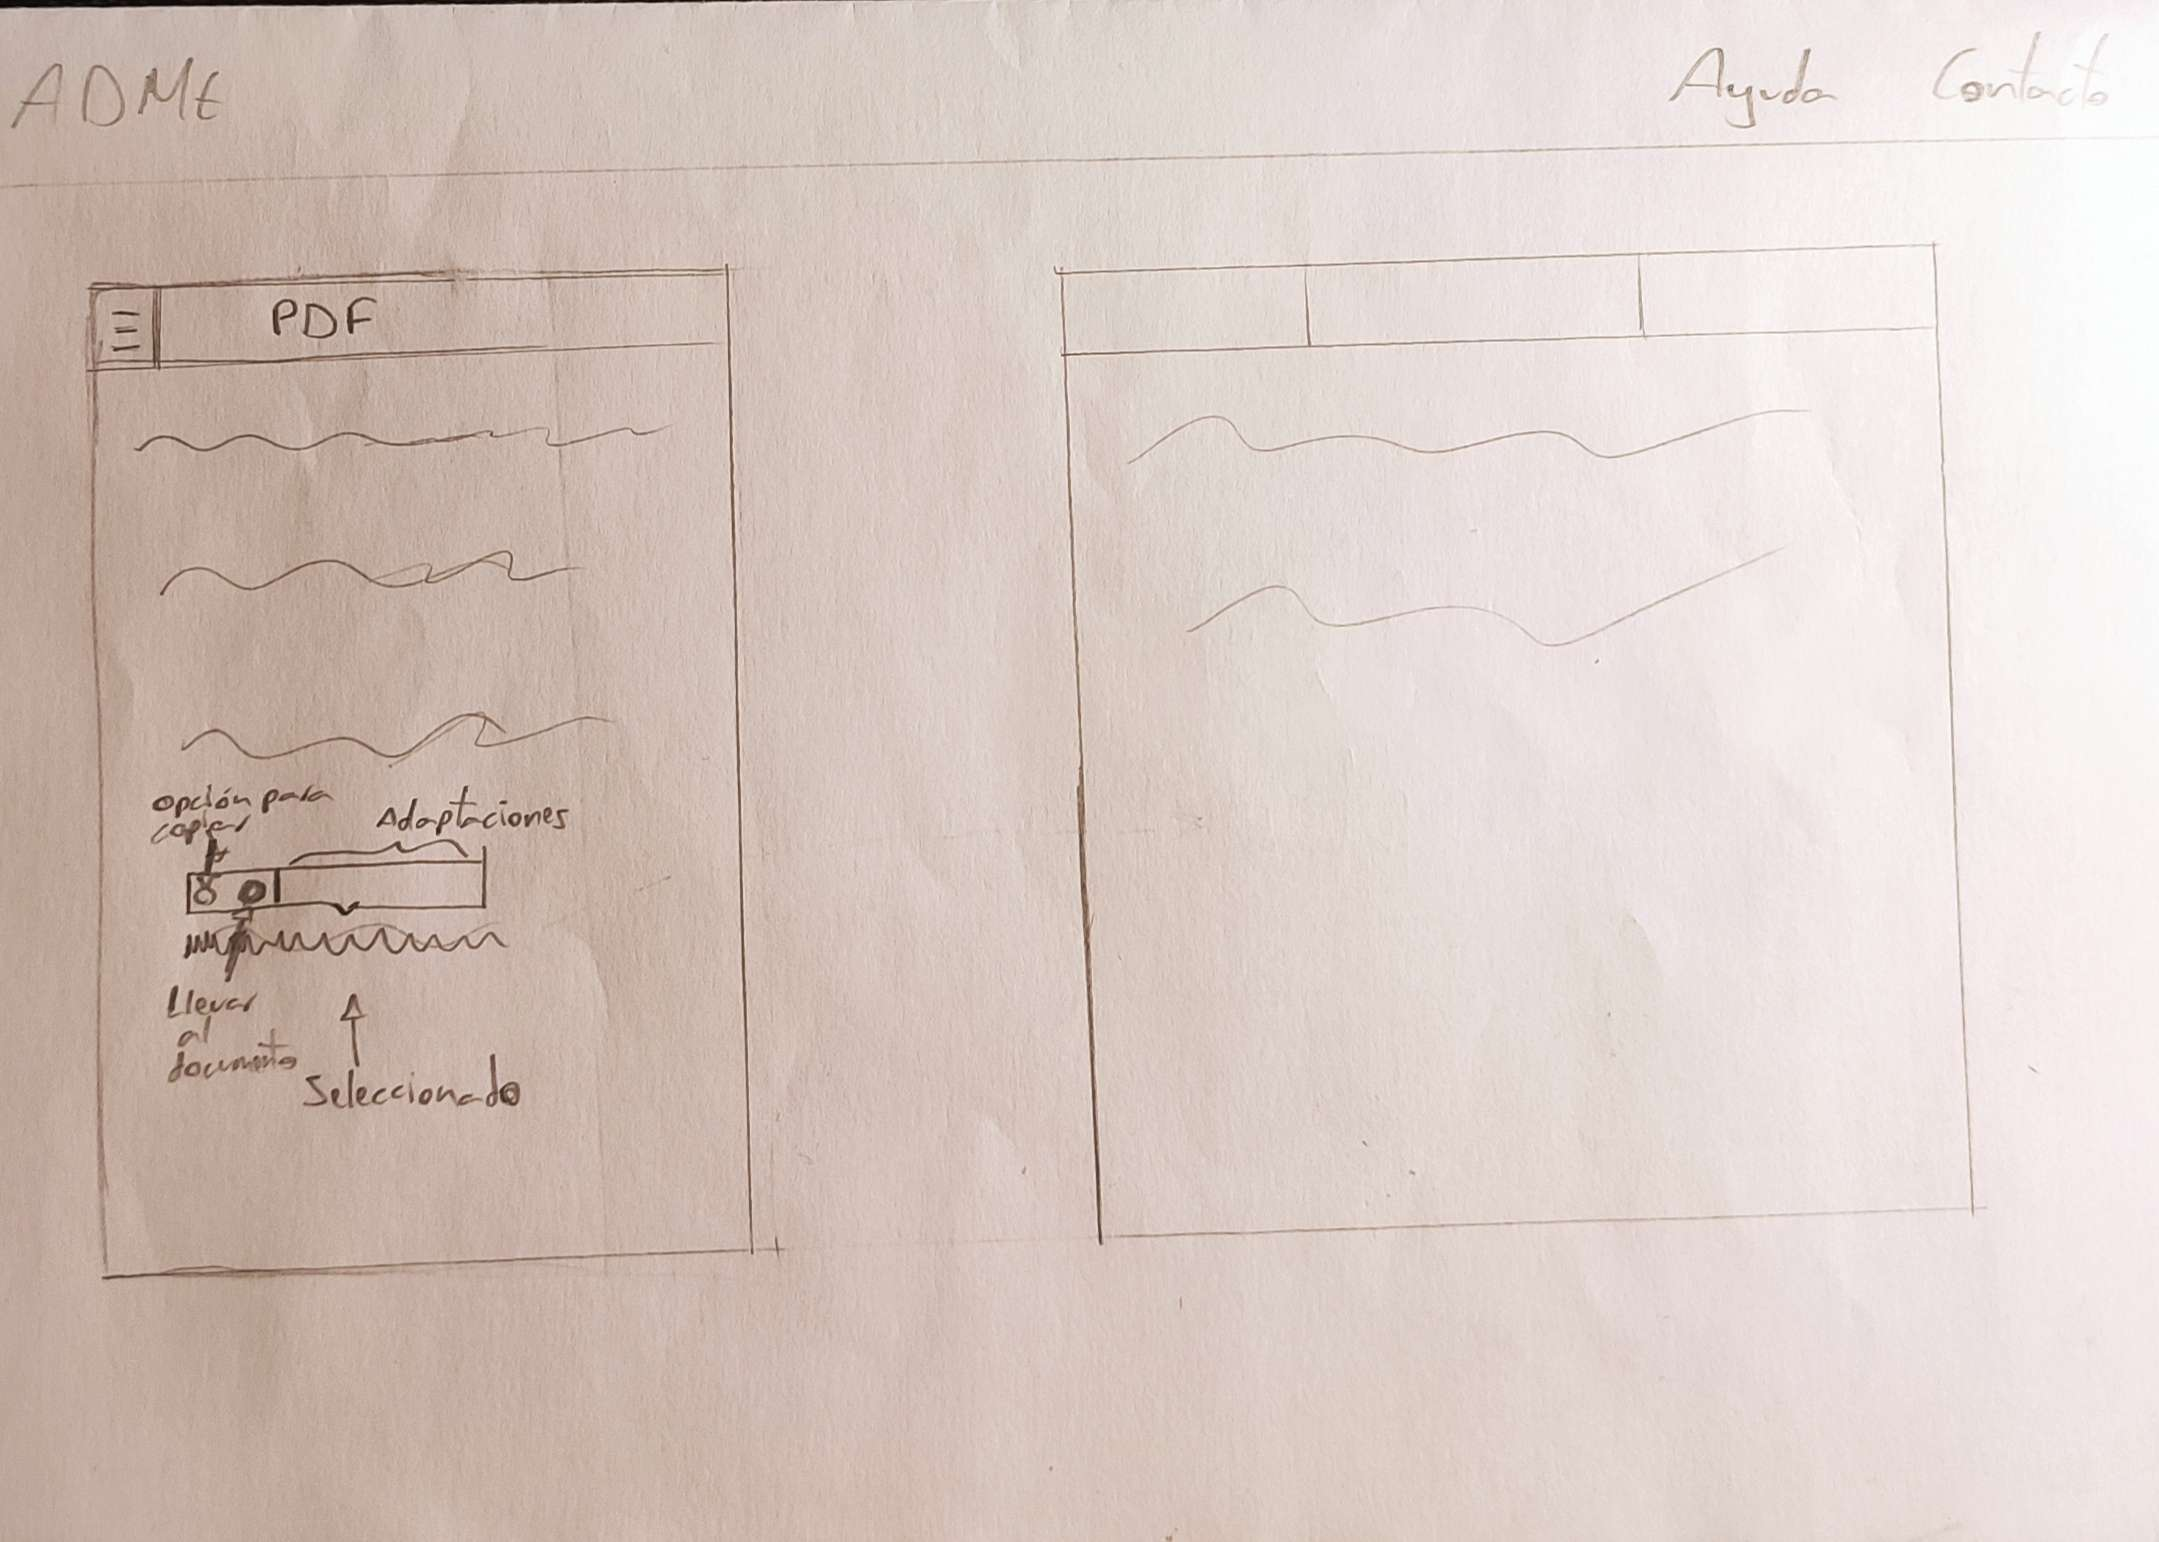
\includegraphics[width=0.7\textwidth]{Diseño/Alvaro/Alvaro02.jpg}
    \caption{Página de inicio con PDF.}
    \label{fig:disenyoAlvaro01b}
  \end{subfigure}

  \caption{Diseño de la página de inicio de Álvaro.}
  \label{fig:disenyoAlvaro01}
\end{figure}

\begin{figure}[ht!]
  \centering
  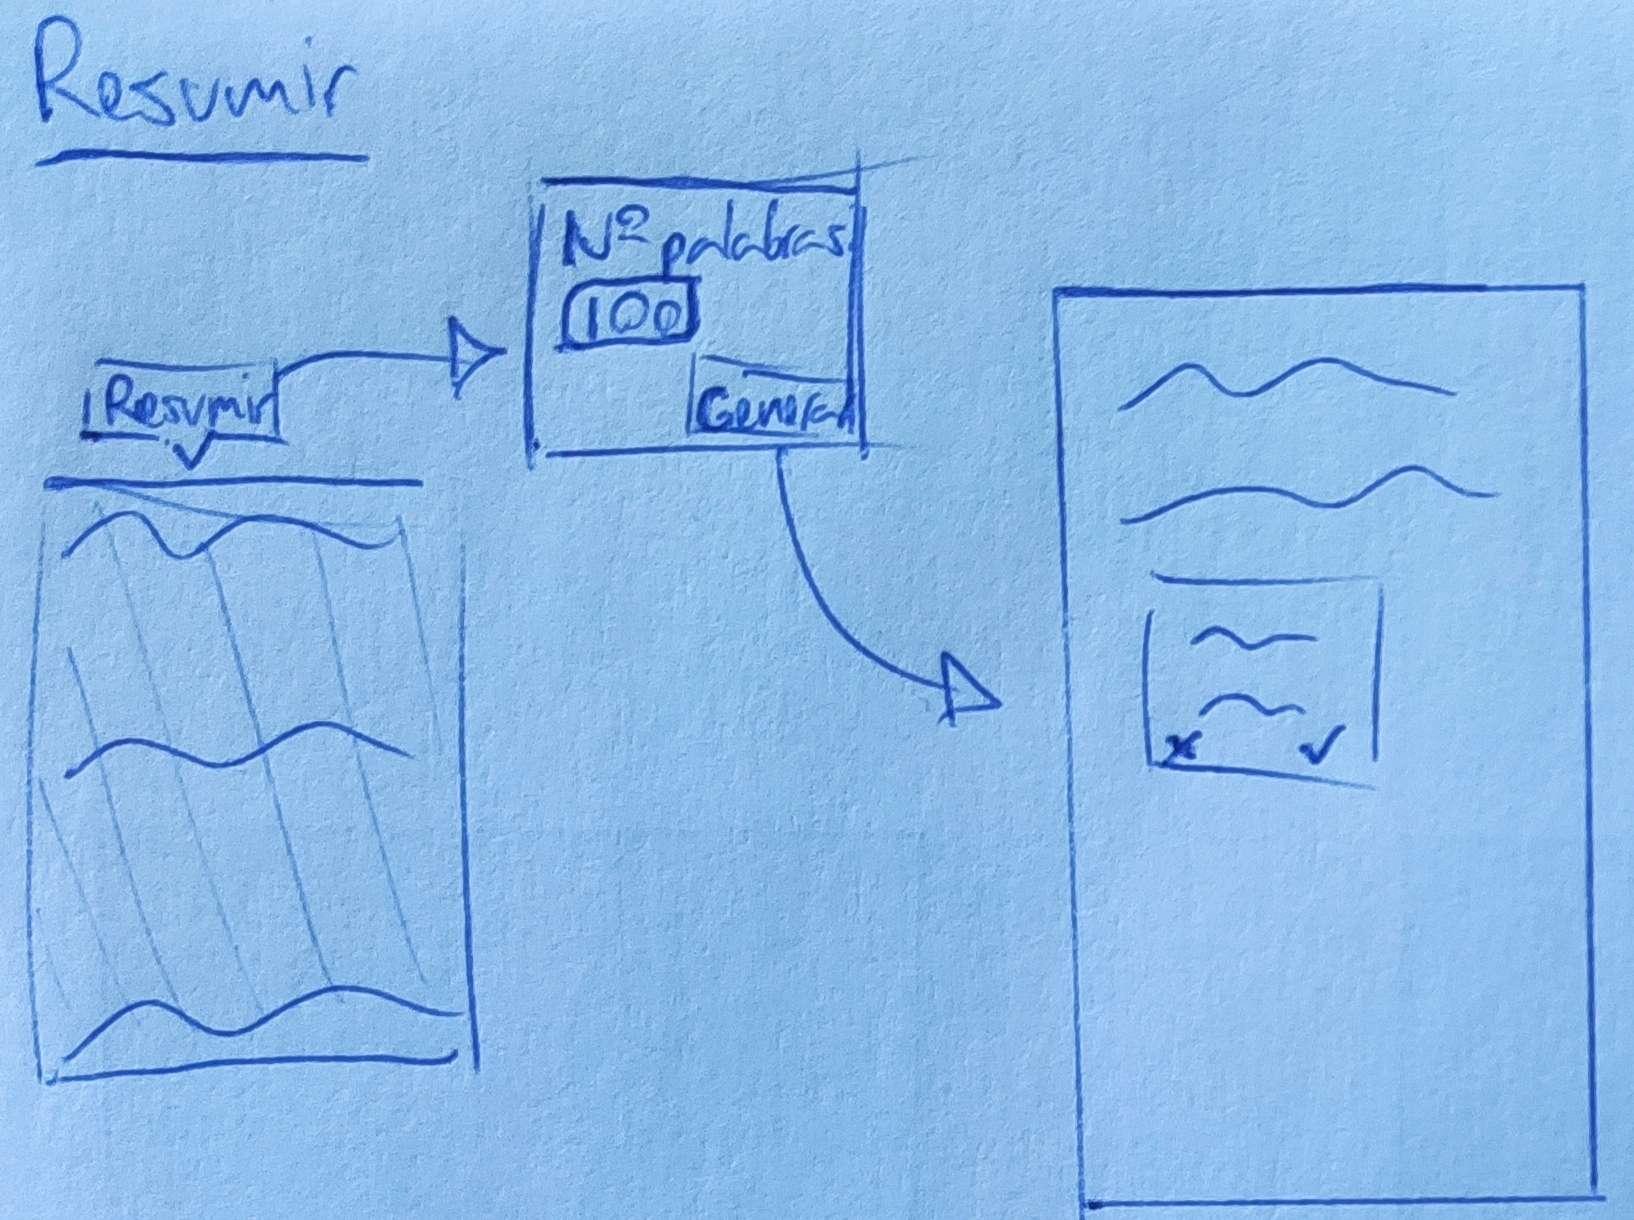
\includegraphics[width=0.6\textwidth]{Diseño/Alvaro/Alvaro03.jpg}
  \caption{Diseño de generar resumen de Álvaro.}
  \label{fig:disenyoAlvaro02}
\end{figure}

\begin{figure}[ht!]
  \centering
  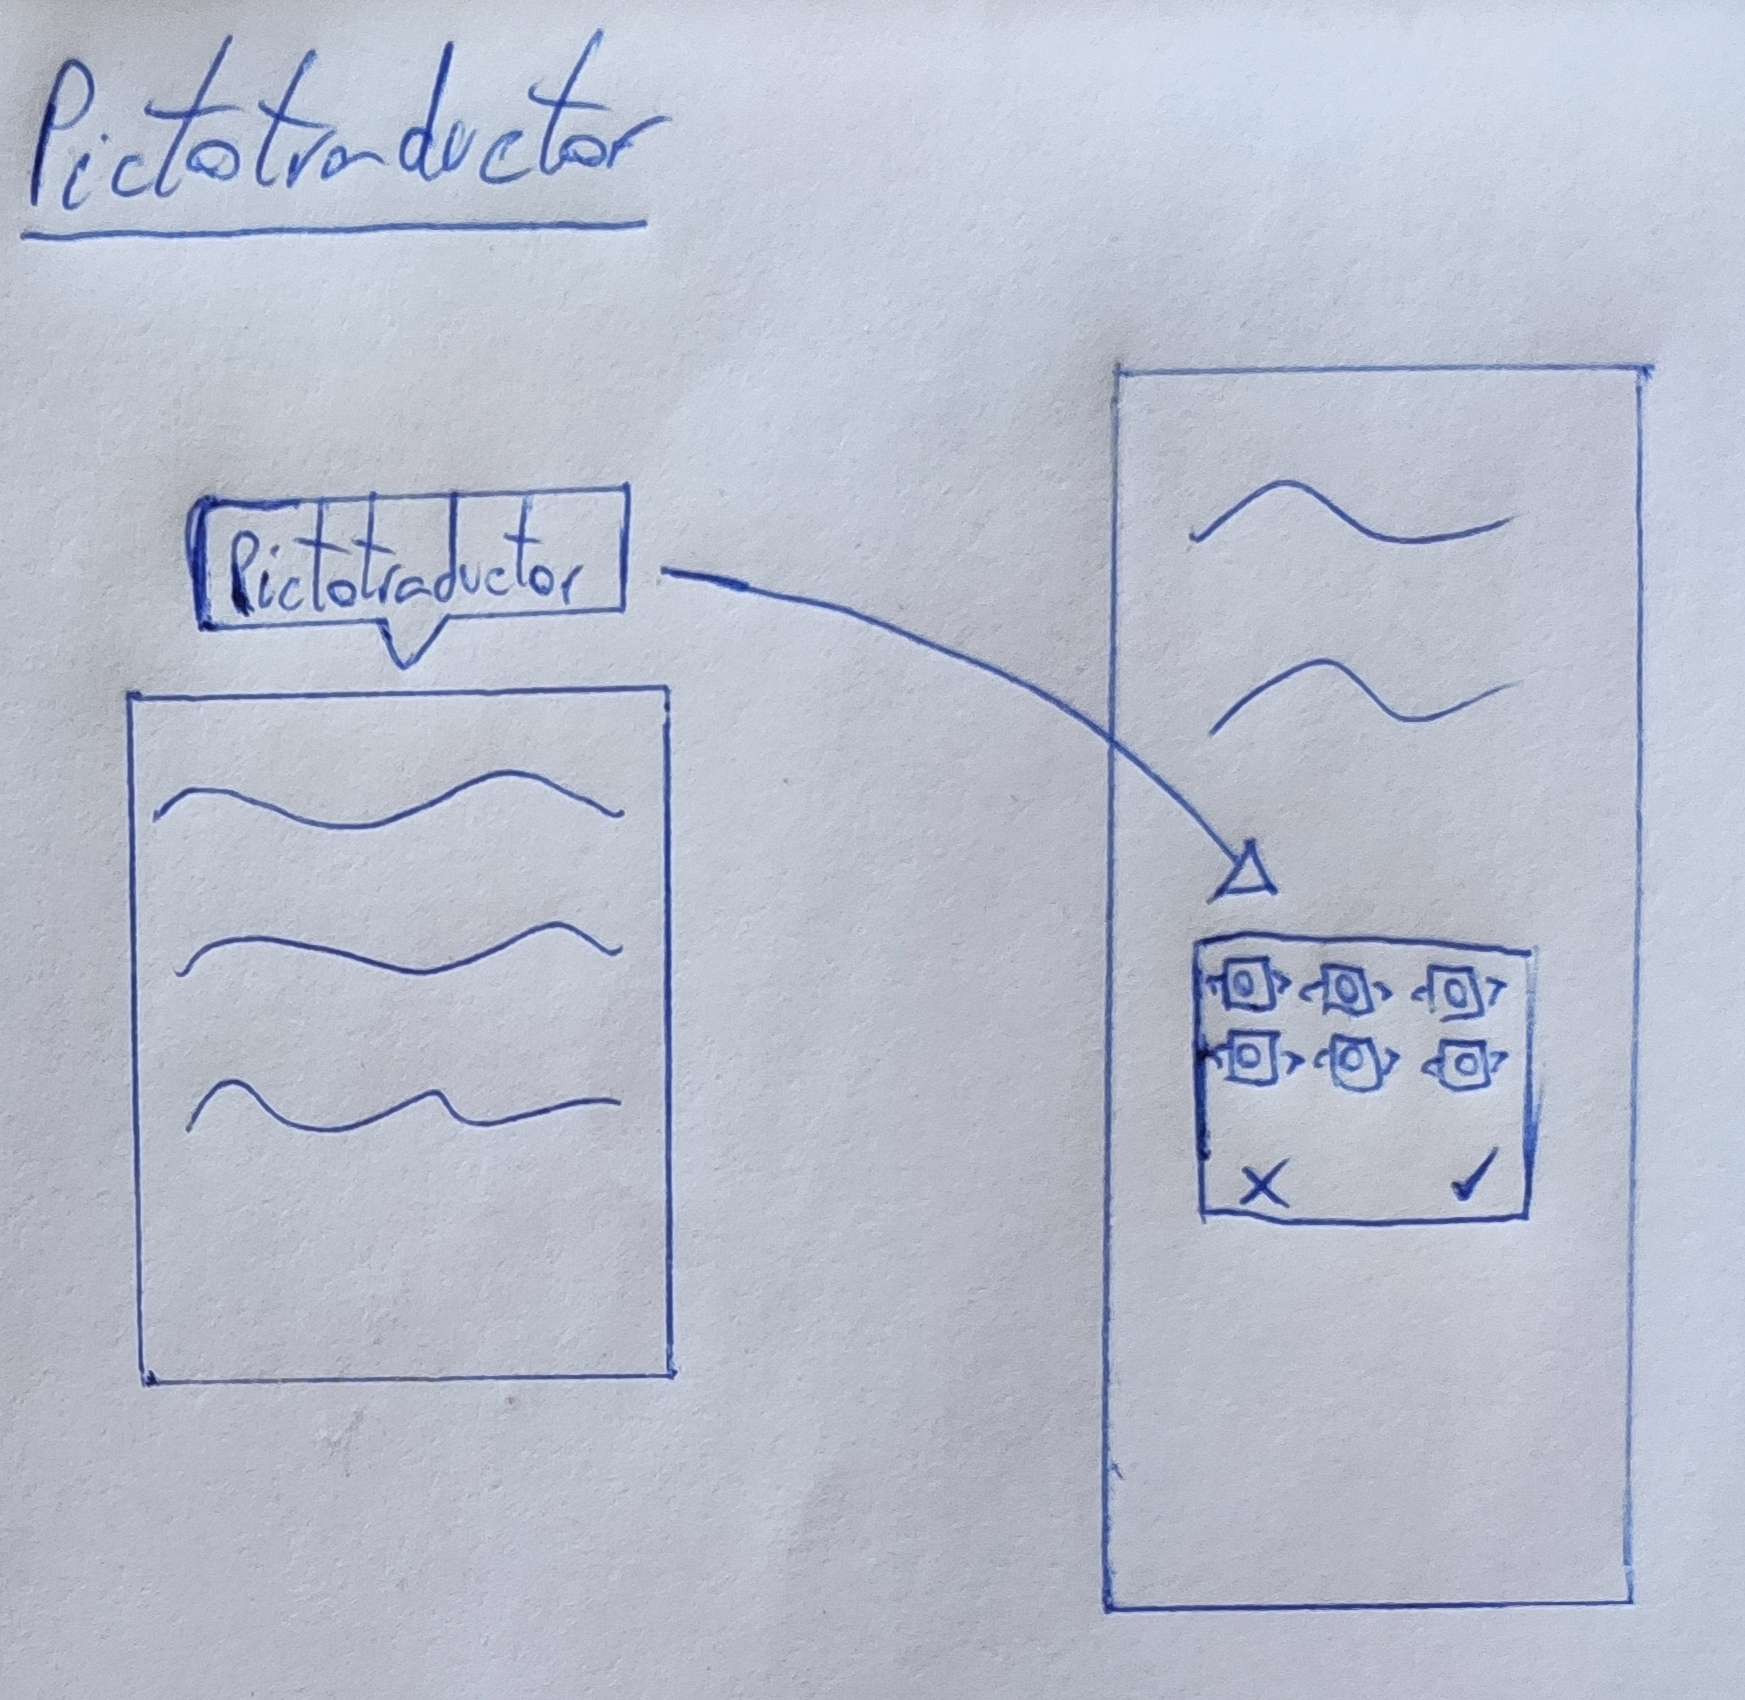
\includegraphics[width=0.5\textwidth]{Diseño/Alvaro/Alvaro04.jpg}
  \caption{Diseño de pictotraductor de Álvaro.}
  \label{fig:disenyoAlvaro03}
\end{figure}

\begin{figure}[ht!]
  \centering
  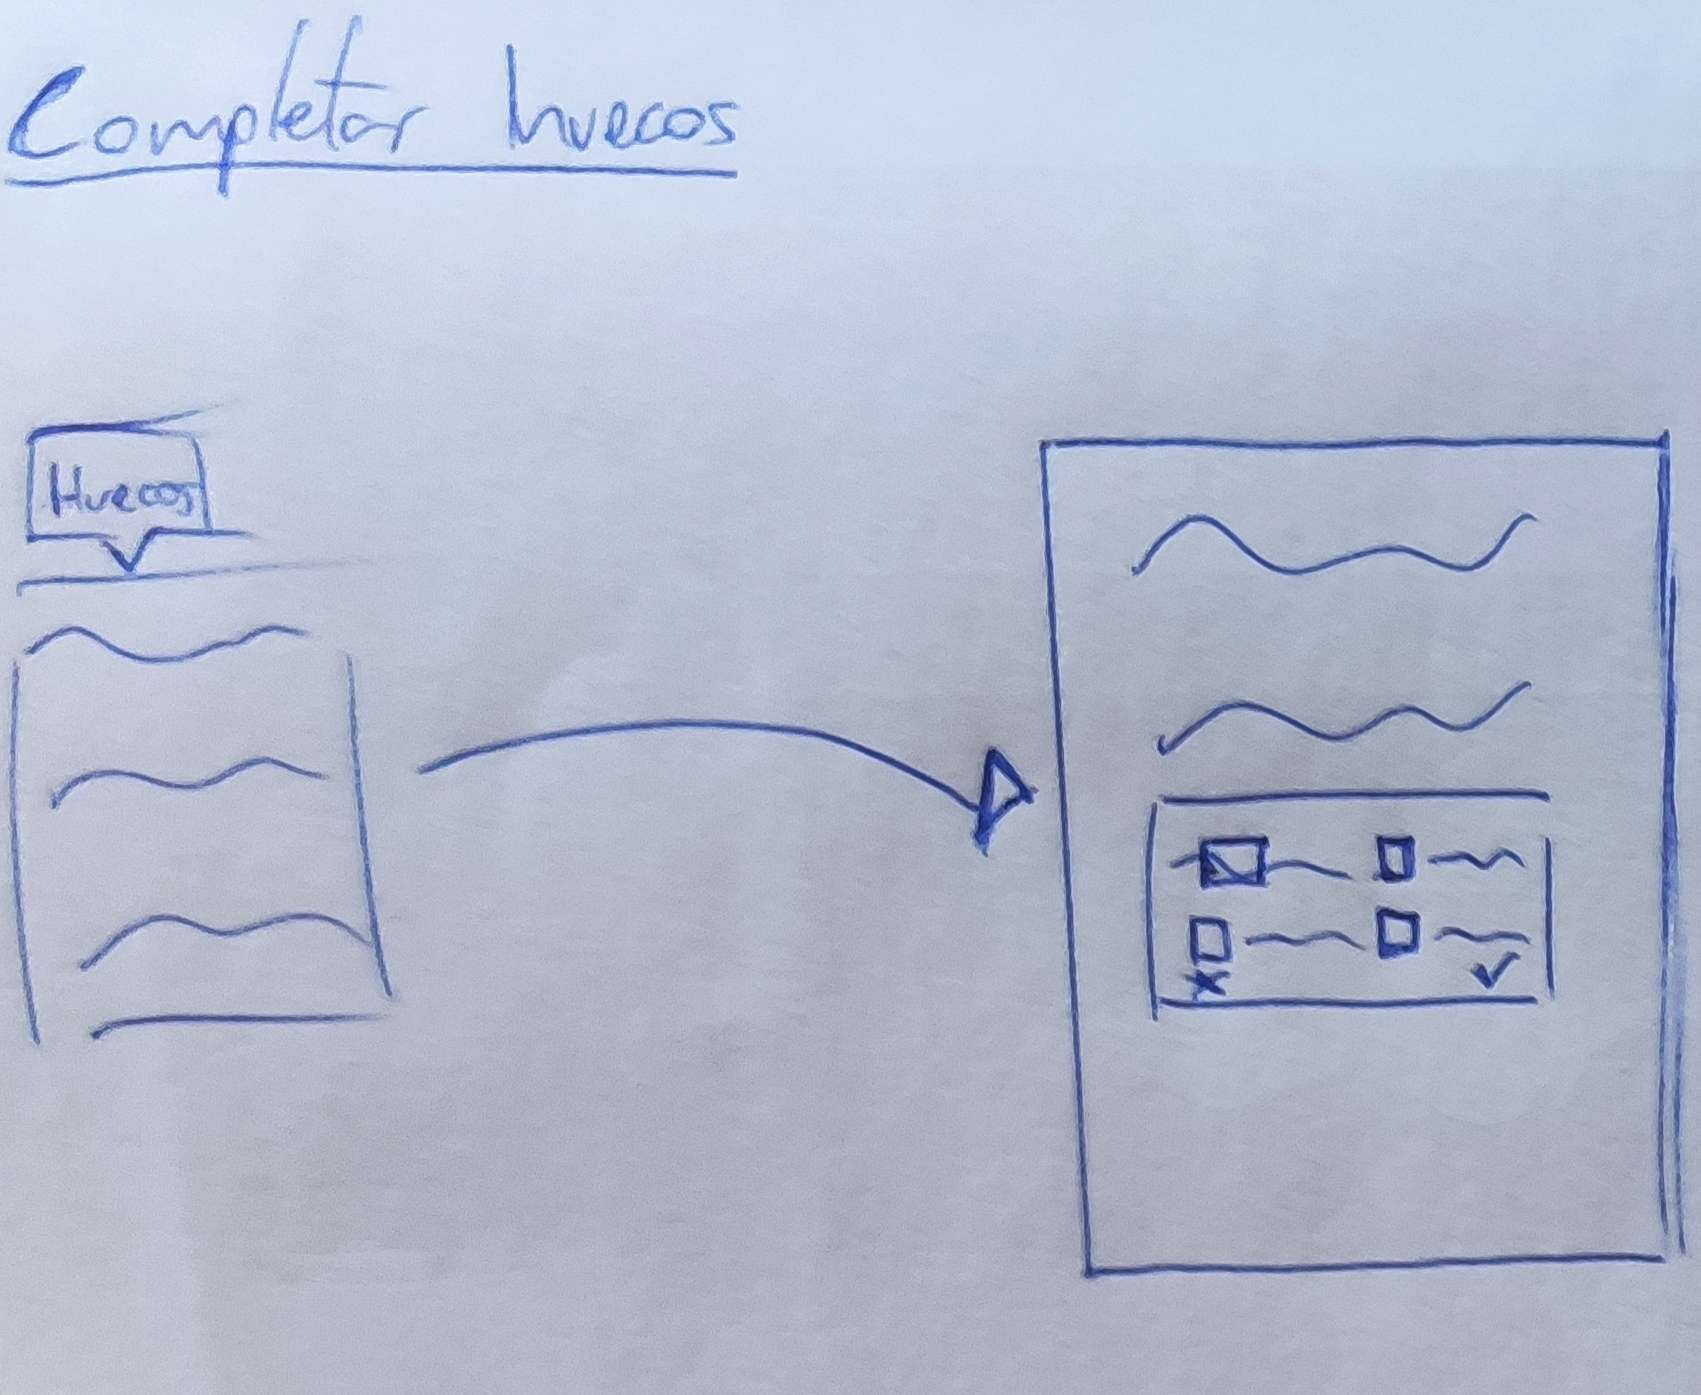
\includegraphics[width=0.5\textwidth]{Diseño/Alvaro/Alvaro05.jpg}
  \caption{Diseño de definir huecos de Álvaro.}
  \label{fig:disenyoAlvaro04}
\end{figure}

\begin{figure}[ht!]
  \centering
  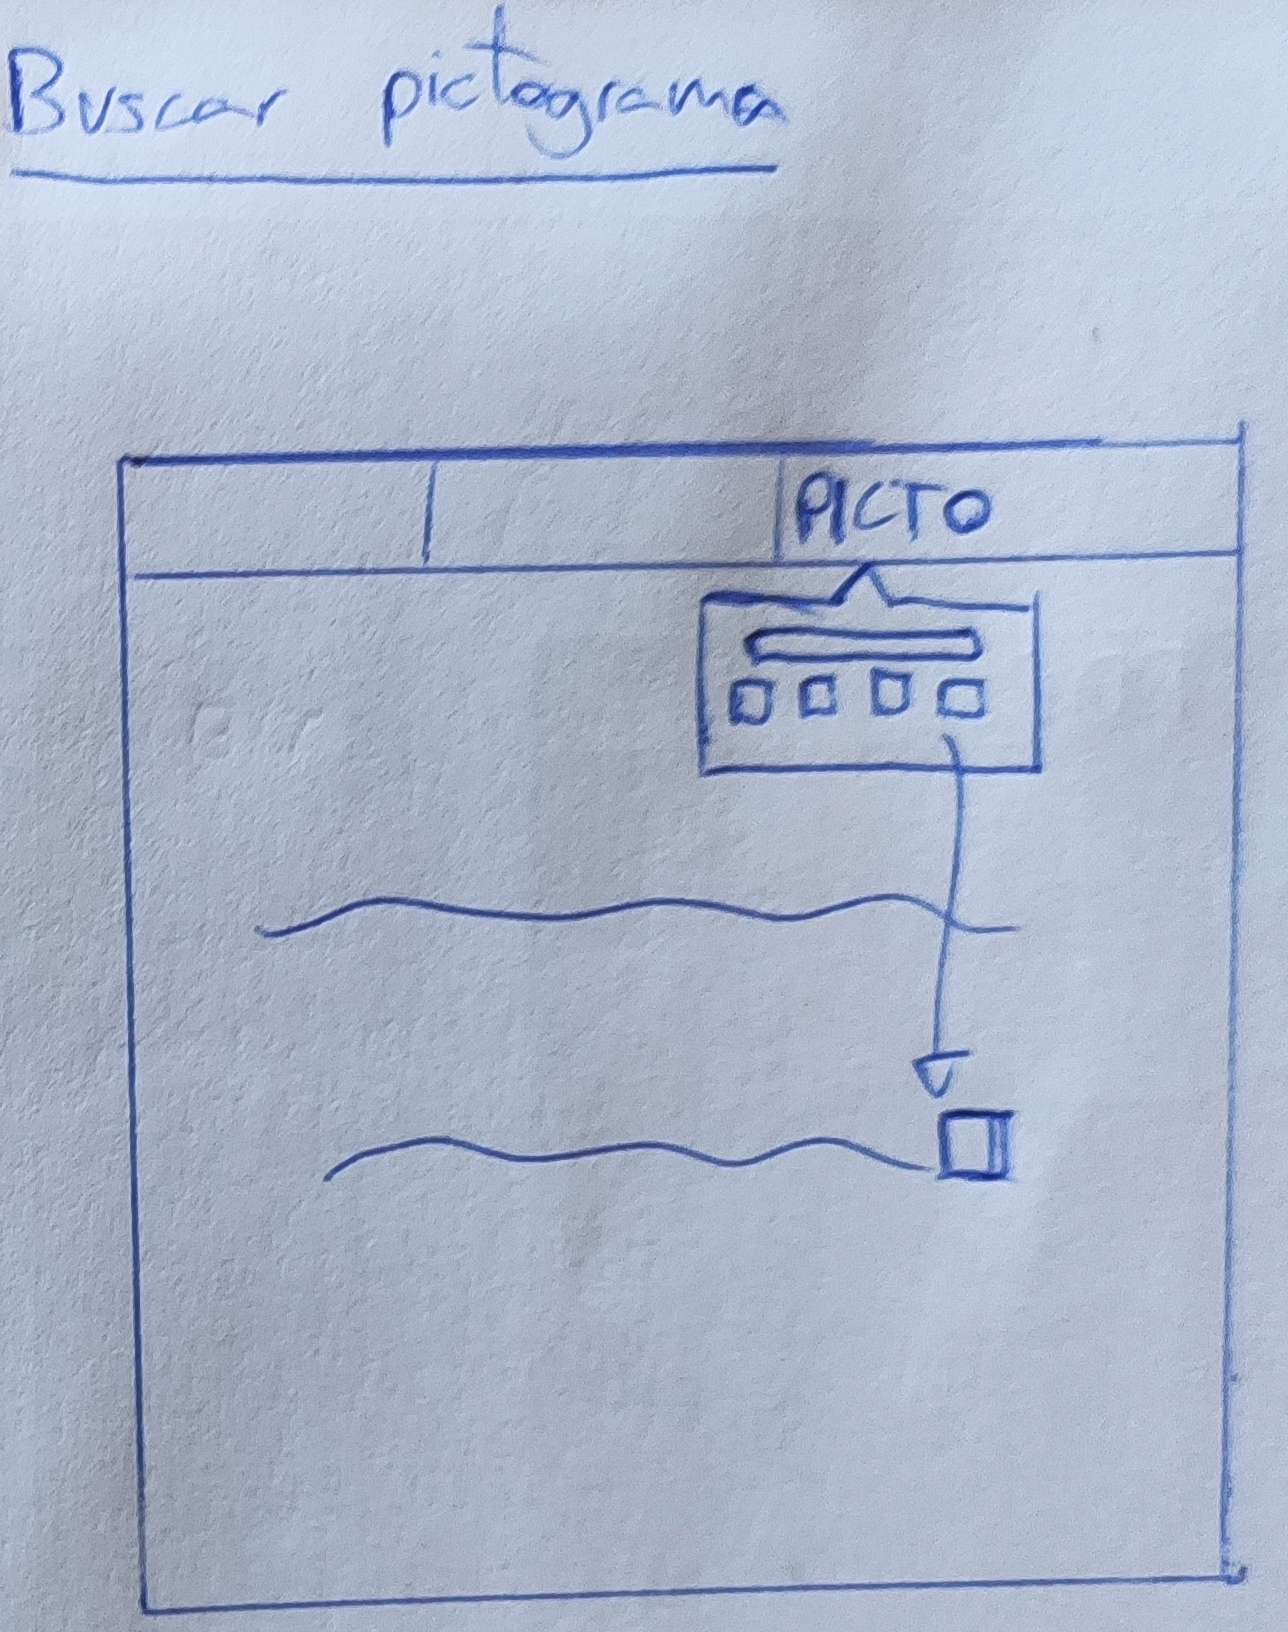
\includegraphics[width=0.6\textwidth]{Diseño/Alvaro/Alvaro06.jpg}
  \caption{Diseño de buscar pictogramas de Álvaro.}
  \label{fig:disenyoAlvaro05}
\end{figure}

\begin{figure}[ht!]
  \centering
  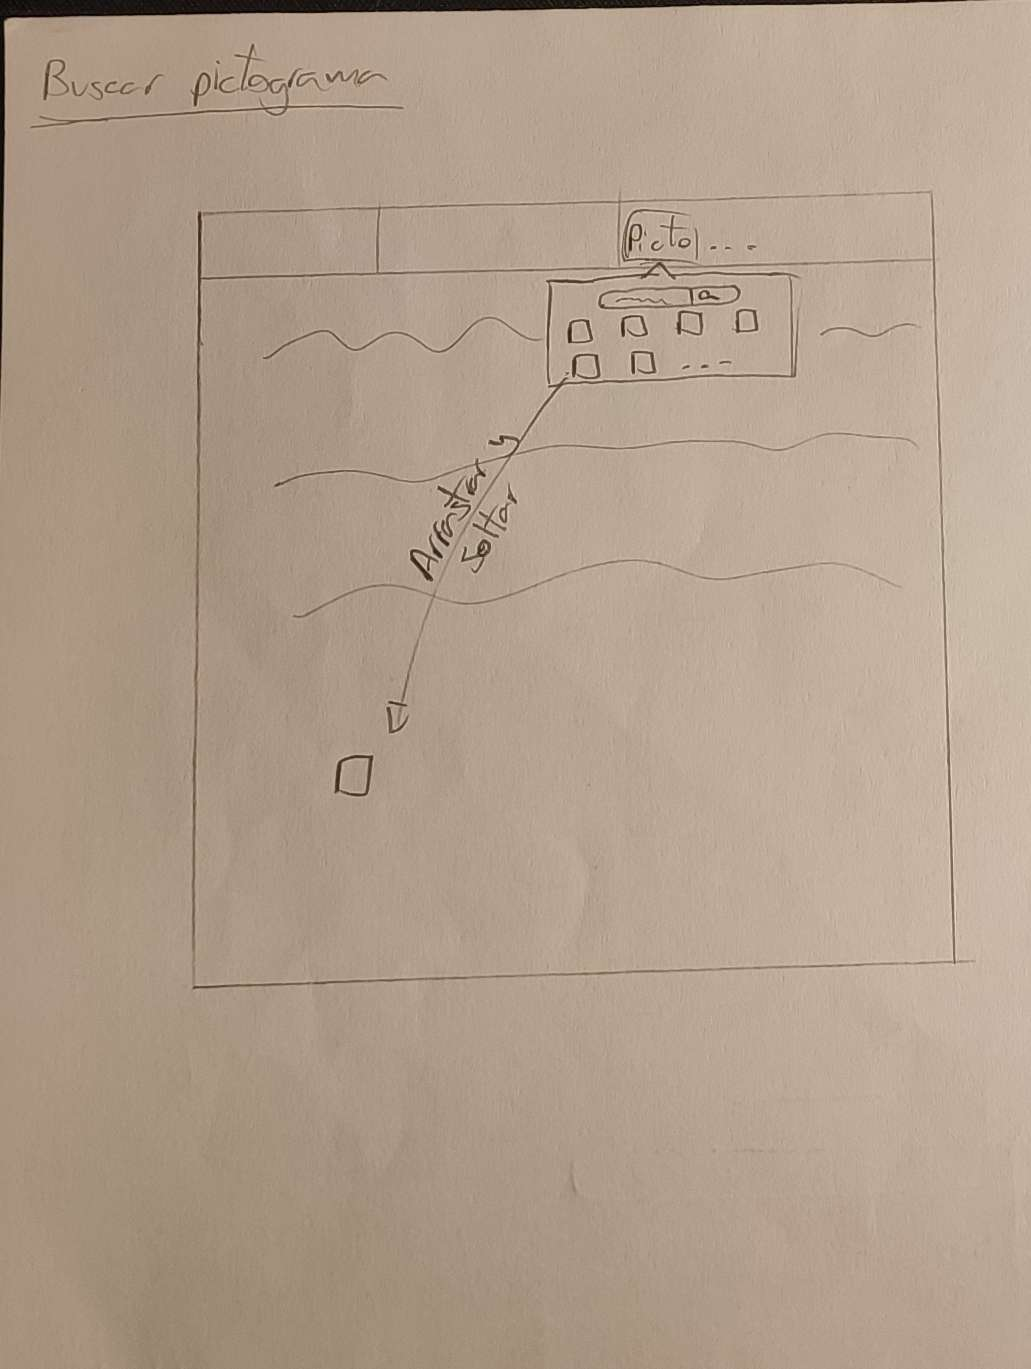
\includegraphics[width=0.6\textwidth]{Diseño/Alvaro/Alvaro07.jpg}
  \caption{Diseño de ejercicio de definiciones de Álvaro.}
  \label{fig:disenyoAlvaro06}
\end{figure}
\chapter{Diseños individuales para la iteración competitiva de Dunia Namour Doughani}
\label{ape:disenyoDunia}

En este apéndice se muestran los diseños individuales realizados por Dunia Namour Doughani para la iteración competitiva. En la Figura \ref{dunia1} se muestra la pantalla de inicio la cual está dividida en 3 secciones, el documento de trabajo, la funcionalidad seleccionada y el PDF cargado. En la Figura \ref{dunia2} se observa la funcionalidad de resumen en la que el usuario pone un texto, pulsa el botón de resumir y le aparece el resumen del texto el cual se puede editar. En cuanto a la Figura \ref{dunia3} se encuentra diseñado el pictotraductor, consta de un campo de texto donde se inserta la frase, al pulsar un botón aparecen los pictogramas. En la Figura \ref{dunia4} se muestra el diseño del ejercicio de flechas que consta de dos columnas, cada una de ellas tiene 2 botones para aumentar o disminuir el número de celdas. En cuanto a la Figura \ref{dunia5} se encuentra representado la funcionalidad de leyenda de colores en la que en un campo de texto se escriben las palabras de la leyenda y a la izquierda de este se encuentra un botón para elegir el color. Finalmente, en la Figura \ref{dunia6} se encuentra diseñado el ejercicio de matemáticas de huecos. En él se elige la longitud de la expresión matemática lo que generará tantos cuadros como longitud se haya puesto y, al pulsar en cada cuadrado aparecerá un desplegable en el que aparecen tanto los números como las operaciones posibles. 

  \begin{figure}[ht!]
    \centering
    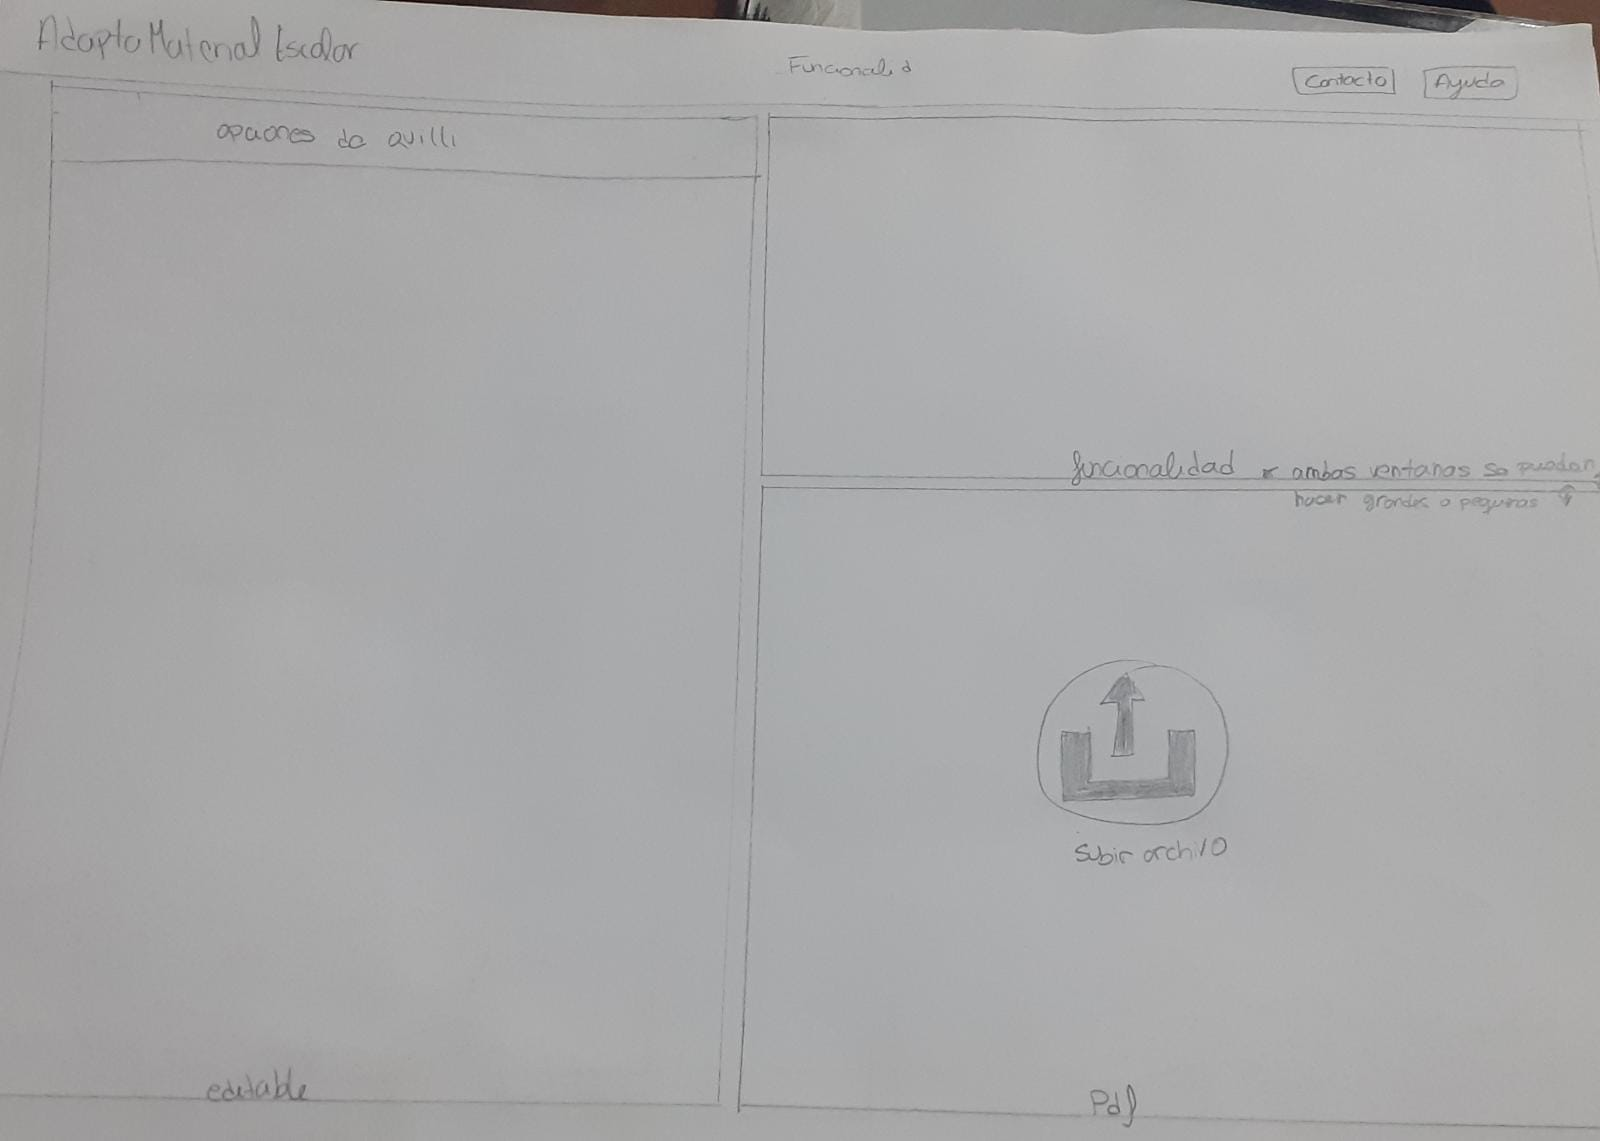
\includegraphics[width=0.6\textwidth]{Diseño/Dunia/principal.jpeg}
    \caption{Diseño pantalla de inicio de Dunia.}
    \label{dunia1}
  \end{figure}

  \begin{figure}[ht!]
    \centering
    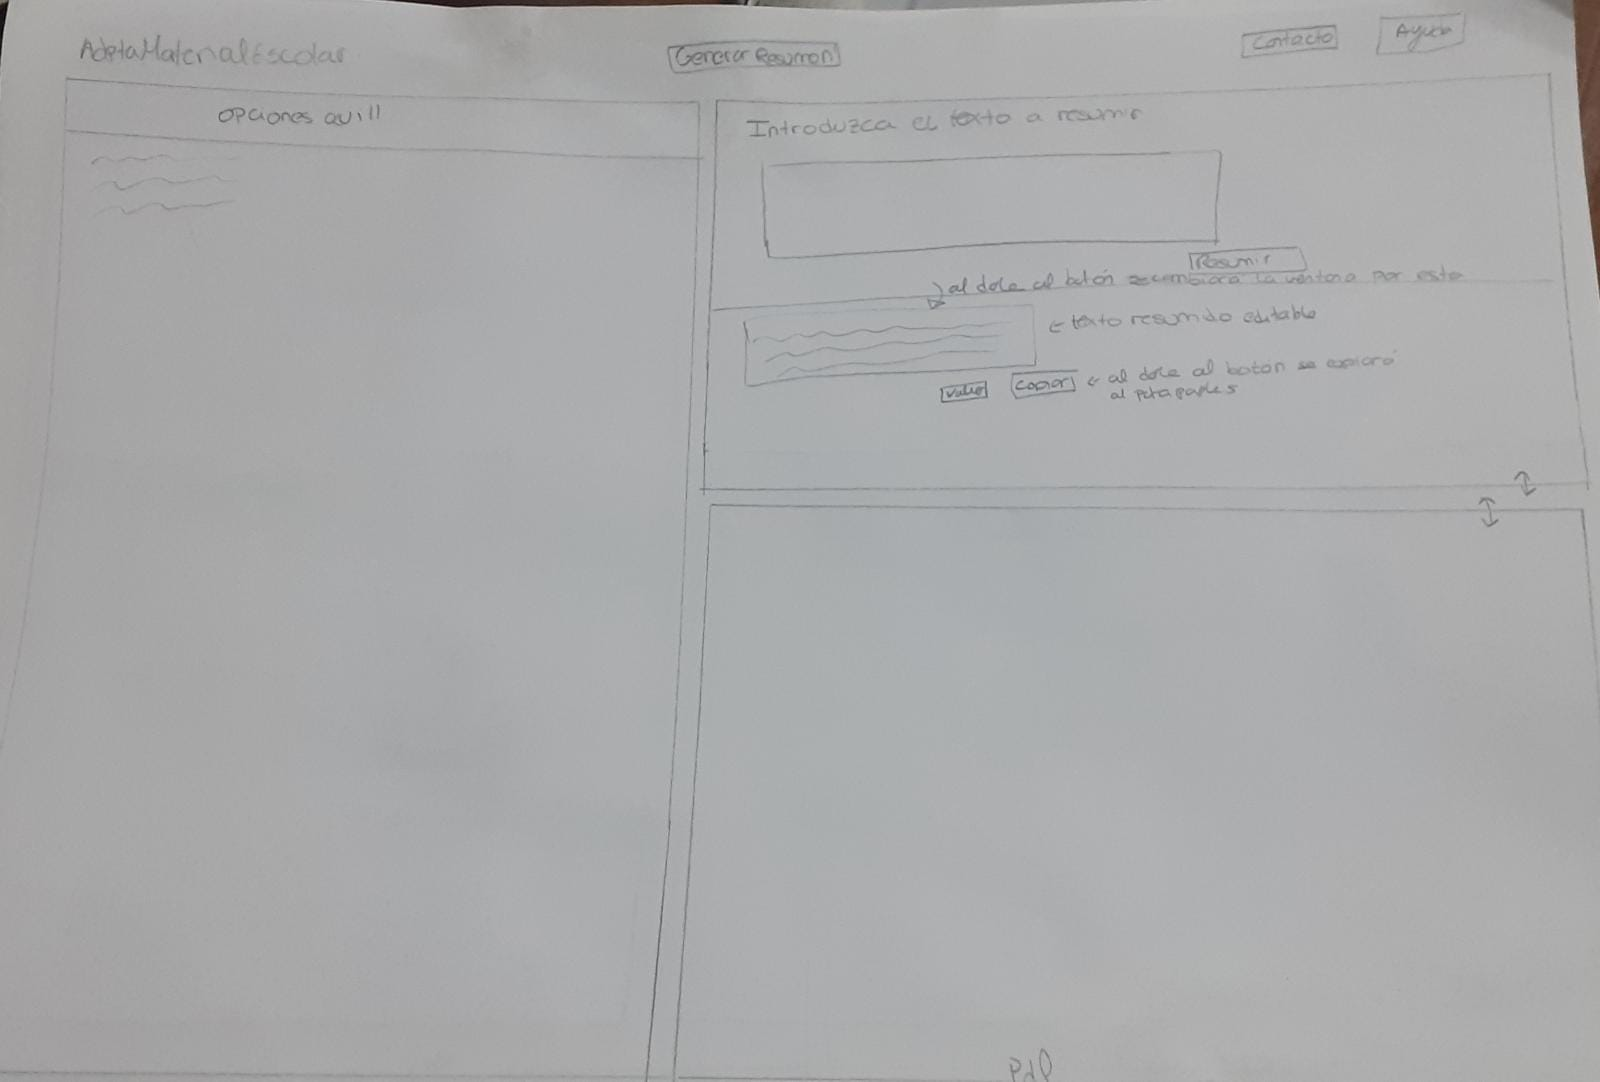
\includegraphics[width=0.6\textwidth]{Diseño/Dunia/resumen.jpeg}
    \caption{Diseño pantalla de generar resumen de Dunia.}
    \label{dunia2}
  \end{figure}

  \begin{figure}[ht!]
    \centering
    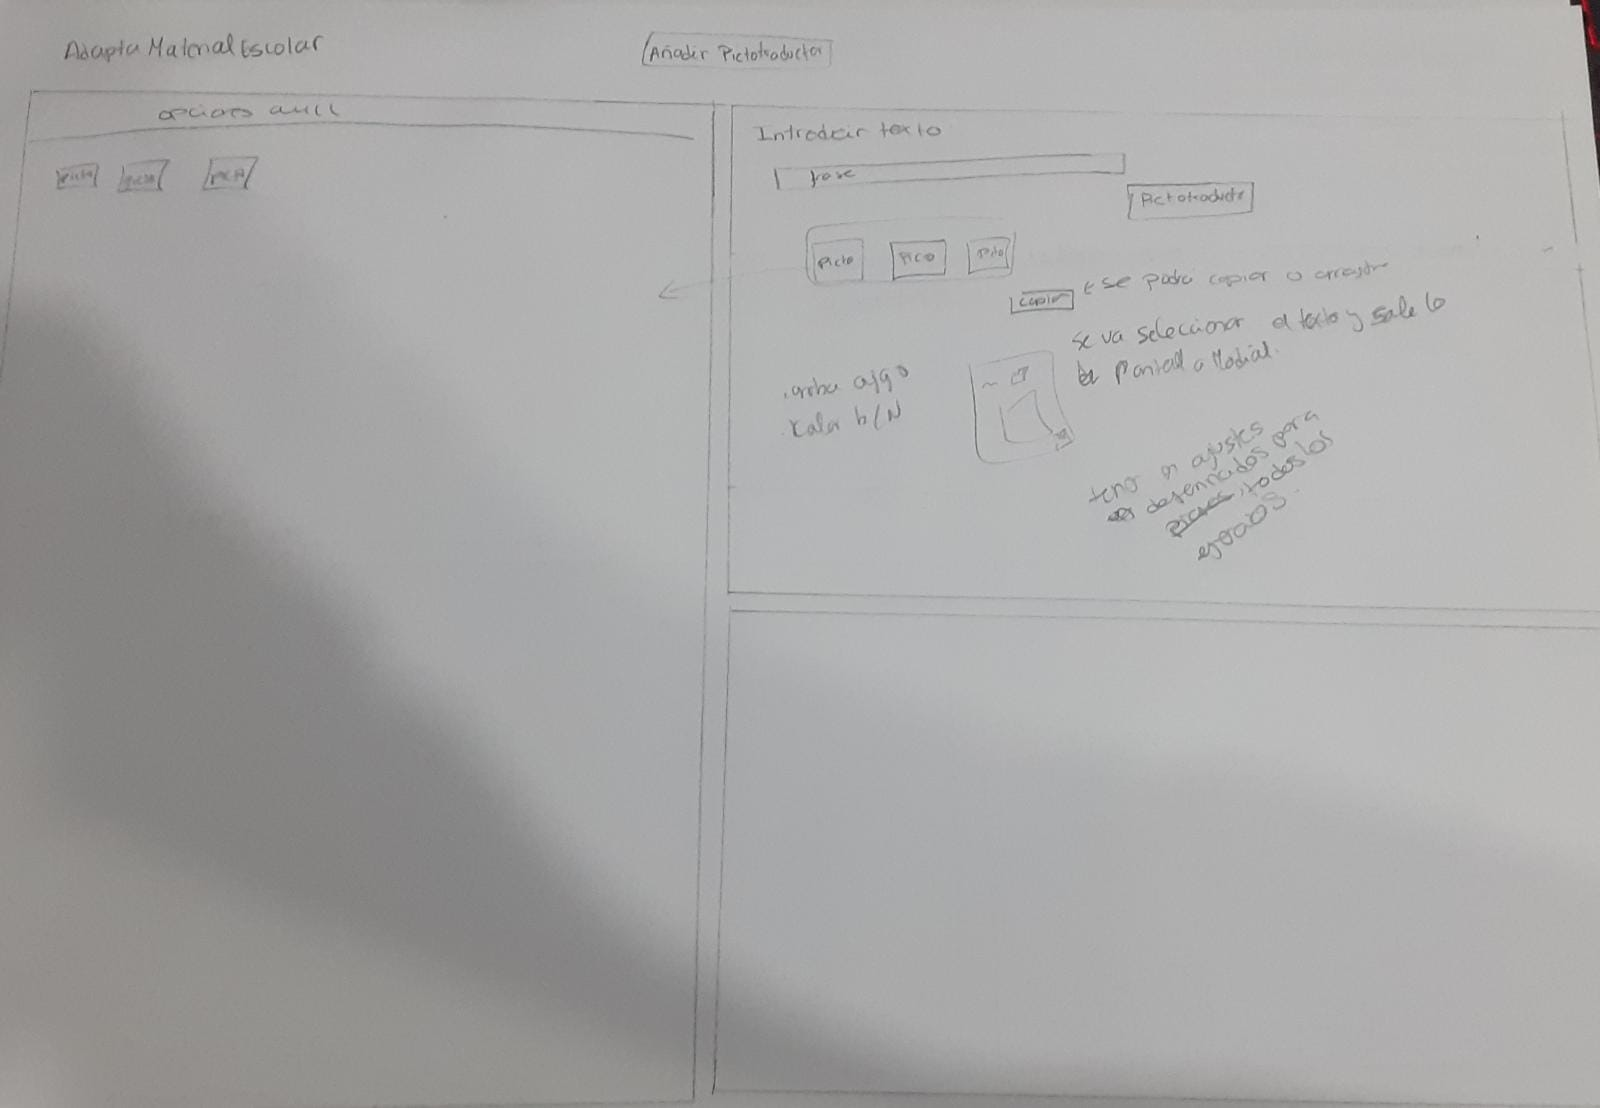
\includegraphics[width=0.6\textwidth]{Diseño/Dunia/picto.jpeg}
    \caption{Diseño de pictotraductor de Dunia.}
    \label{dunia3}
  \end{figure}

  \begin{figure}[ht!]
    \centering
    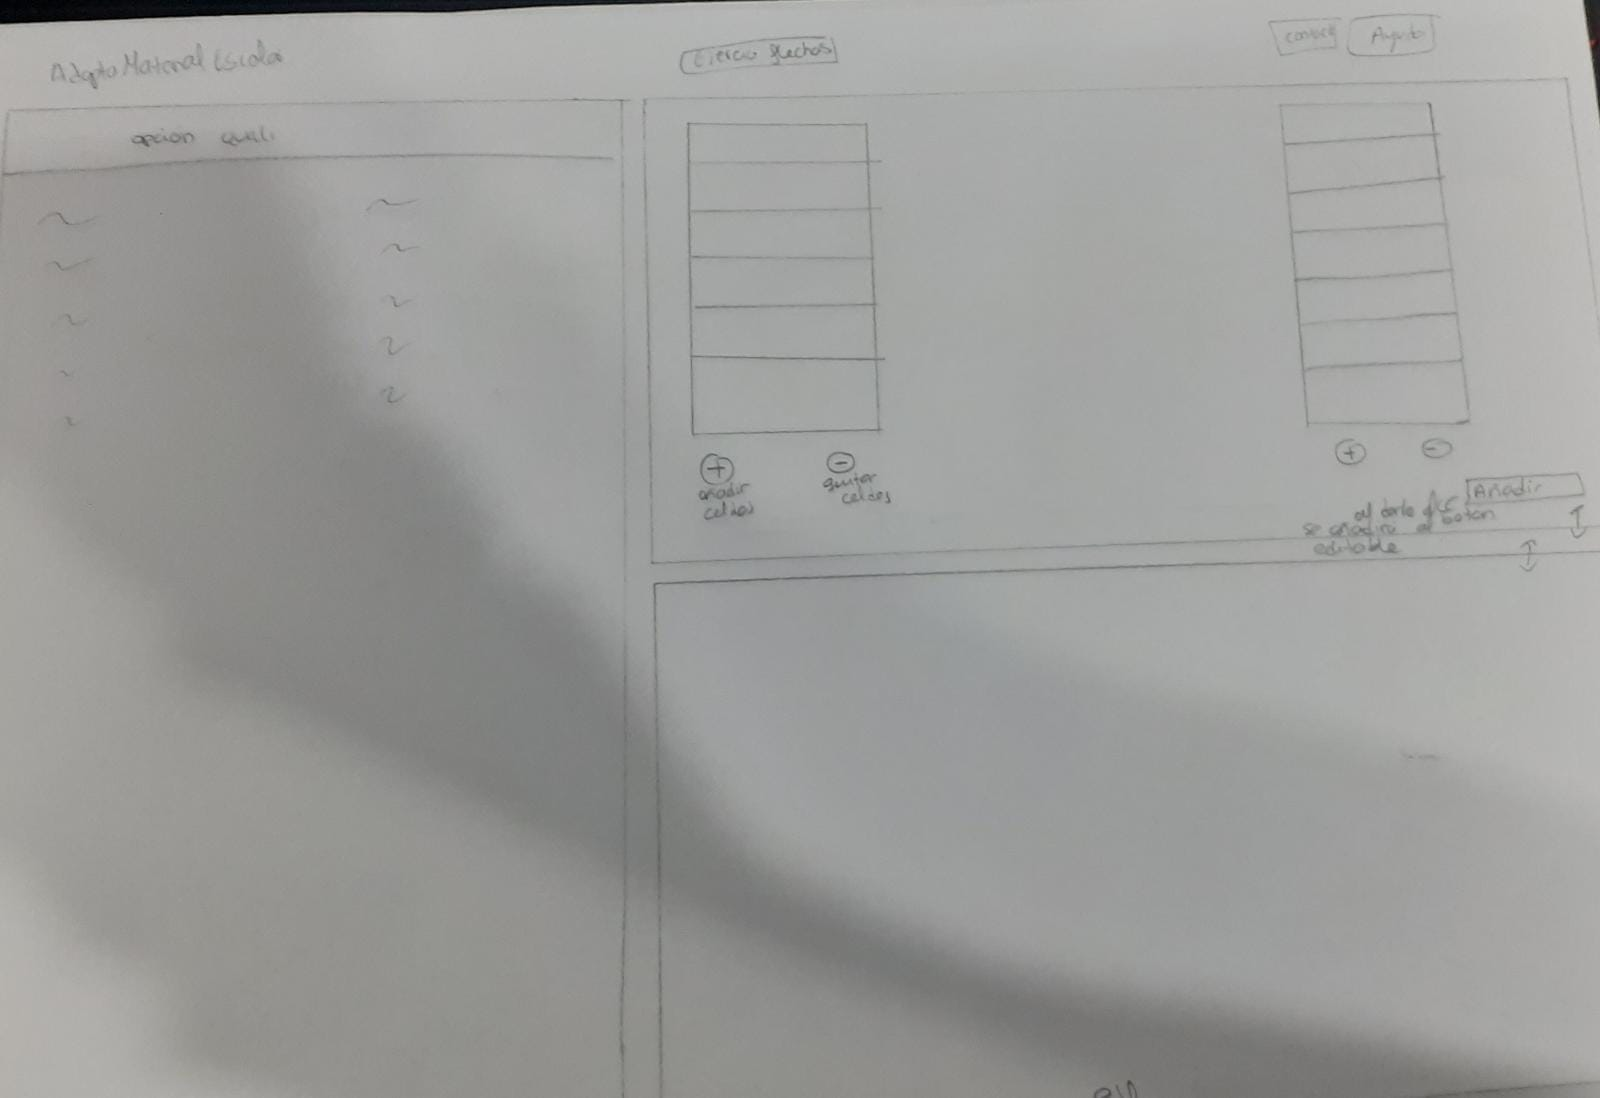
\includegraphics[width=0.7\textwidth]{Diseño/Dunia/flechas.jpeg}
    \caption{Diseño de ejercicios de flechas de Dunia.}
    \label{dunia4}
  \end{figure}

  \begin{figure}[ht!]
    \centering
    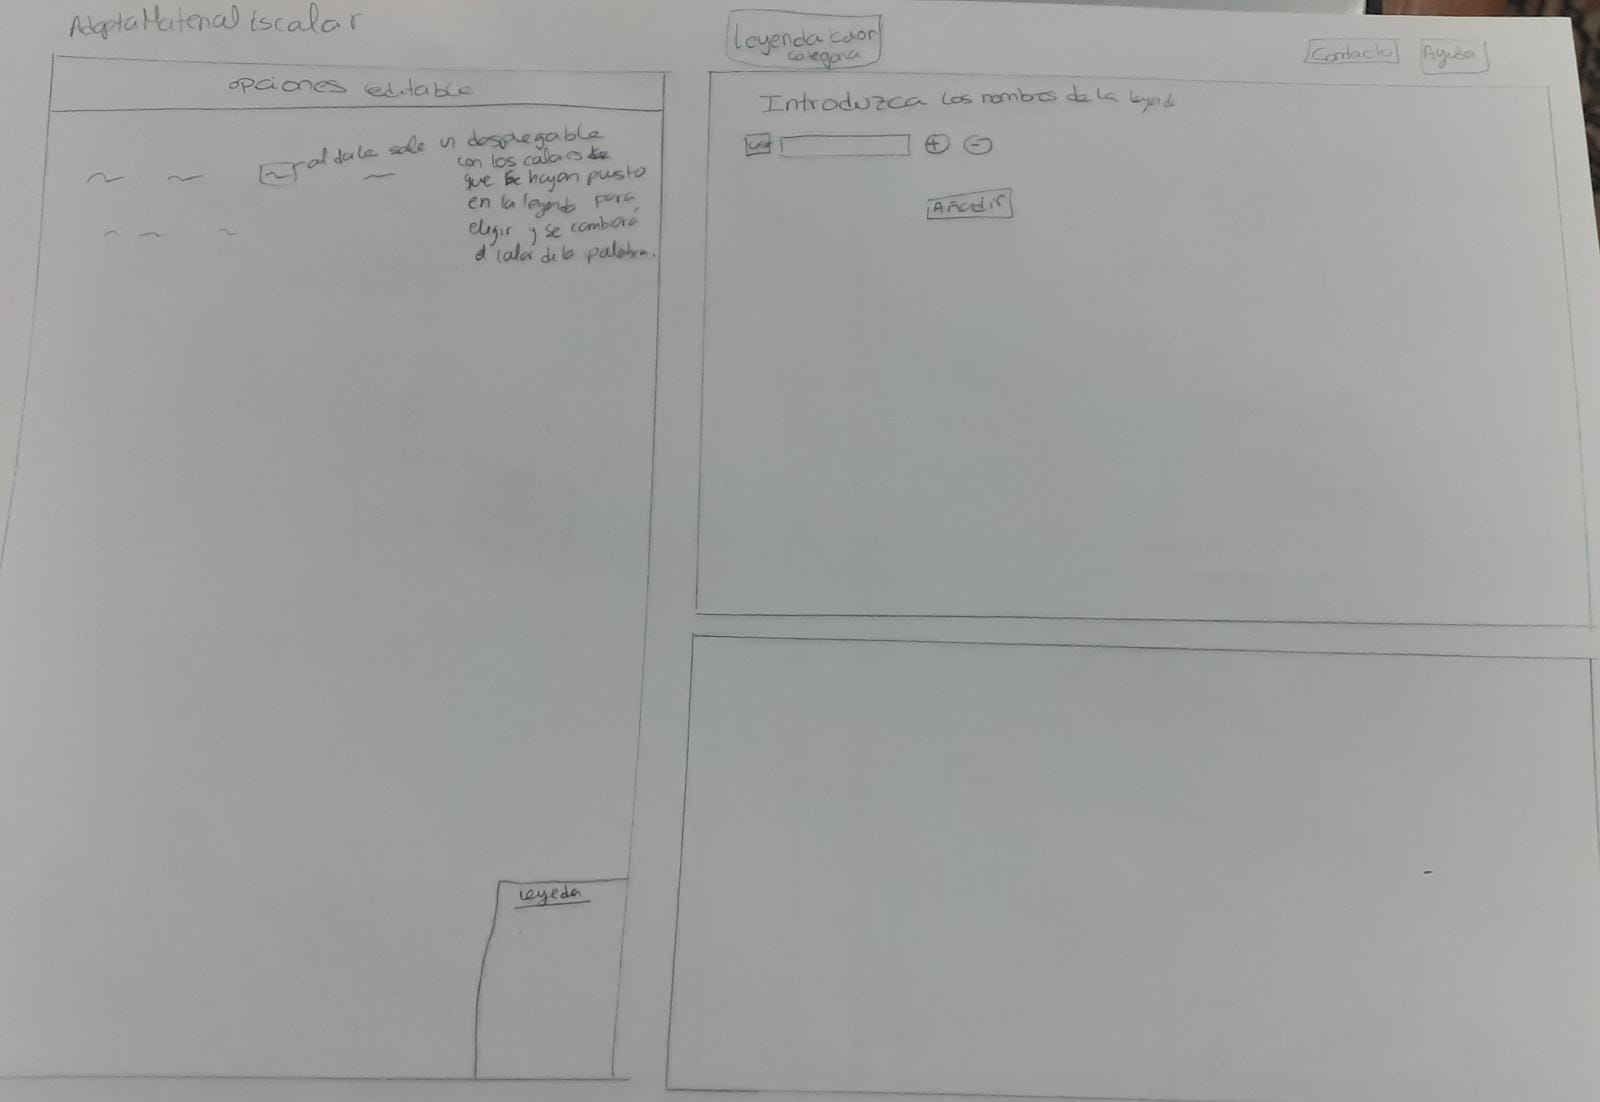
\includegraphics[width=0.7\textwidth]{Diseño/Dunia/leyendaColor.jpeg}
    \caption{Diseño de leyenda de colores de Dunia.}
    \label{dunia5}
  \end{figure}

  \begin{figure}[ht!]
    \centering
    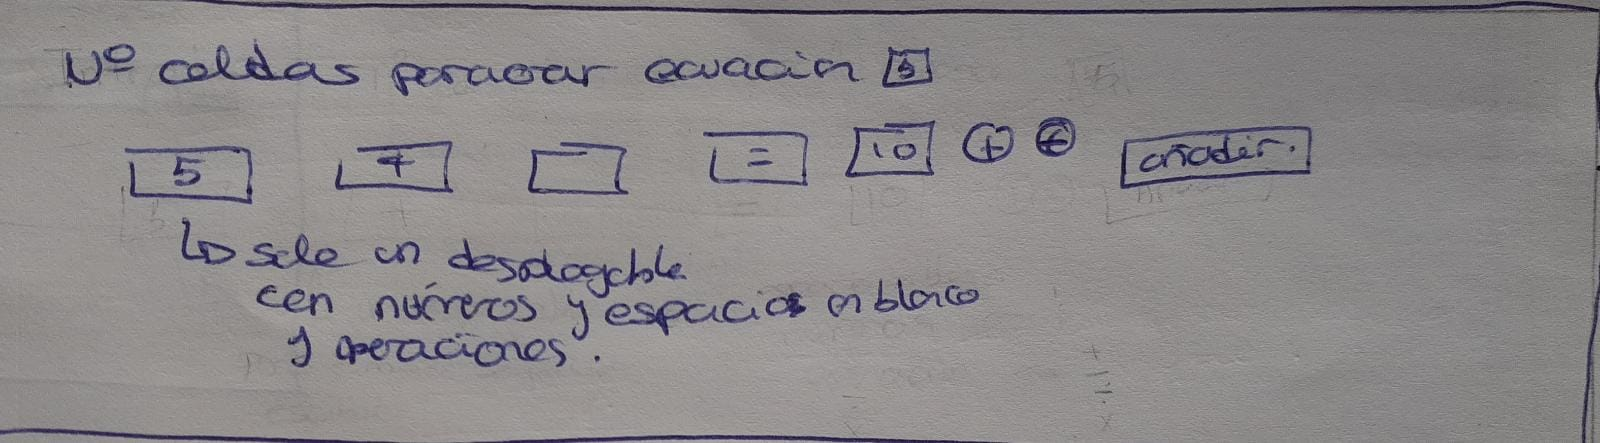
\includegraphics[width=0.7\textwidth]{Diseño/Dunia/hueco.jpeg}
    \caption{Diseño de ejercicios matemáticas de huecos de Dunia.}
    \label{dunia6}
  \end{figure}
\chapter{Diseños individuales para la iteración competitiva de Alberto Alejandro Rivas Fernandez}
\label{ape:disenyoAlberto}

En este apéndice se muestran los diseños individuales realizados por Alberto Alejandro Rivas Fernandez para la iteración competitiva.

En primer lugar, en la figura \ref{AlbertoPaginaPrincipal1} se muestra la página principal antes de haber seleccionado un documento PDF, por lo que hay un elemento en el que podemos subir un fichero. Luego en la figura \ref{AlbertoPaginaPrincipal2}  tenemos la página principal después de haber seleccionado un documento, en la parte izquierda se muestra dicho documento, y en la parte izquierda tenemos el editor de texto con todos los botones para acceder a las funcionalidades en la parte superior. 

En la figura \ref{Alberto13} se muestra el ejercicio de huecos, en el que el usuario puede escribir un texto y seleccionar qué palabras quiere sustituir por un hueco. En la figura \ref{Alberto14} se observa el ejercicio de definiciones, en el que el usuario puede añadir una serie de definiciones e indicar la cantidad de líneas que quiere insertar para cada definición, junto con otras opciones. En la figura \ref{Alberto15} está el ejercicio de desarrollo, que consta de un área de texto en la que se puede escribir el enunciado del ejercicio, también se puede indicar la cantidad de líneas cómo en la figura anterior, junto con otras opciones. En la figura \ref{Alberto16} se presenta el ejercicio de sopa de letras, en el que se puede indicar el número de filas, columnas y palabras, para luego insertar las palabras que se quieren mostrar en la sopa de letras. En la figura \ref{Alberto17} se encuentra el ejercicio de verdadero y falso, que consta de un input con el que el usuario puede añadir las frases que quiera insertar en el ejercicio. En la figura \ref{Alberto1} se muestra la leyenda de colores, que permite añadir una serie de frases acompañadas de un color que puede ser seleccionado por el usuario. En la figura \ref{Alberto2} se observa la leyenda de colores por asignatura, en este caso hay un solo selector de color, este color se usará para añadir un borde a la página, el cual indica la asignatura a la que pertenece. En la figura \ref{Alberto3} está el modal para crear una cuadrícula, este simplemente consta de un input en el que se puede indicar el número de filas que se quiere tener en la cuadrícula. En la figura \ref{Alberto4} se presenta el modal para crear insertar líneas doble pauta en el documento, este simplemente consta de un input en el que se puede indicar el número de líneas que se quieren insertar. En la figura \ref{Alberto5} se encuentra el ejercicio de flechas, el cual tiene dos columnas con varios inputs donde el usuario puede escribir los conceptos a relacionar, también tiene un botón en la parte inferior para añadir nuevas filas. En la figura \ref{Alberto6} se muestra el ejercicio de matemática con huecos, este modal consta de un campo de texto en el que se puede escribir una fórmula con LaTeX. En la figura \ref{Alberto8} se observa el modal de generar resumen, en este hay un campo en el que el usuario puede insertar un texto, y al dar click al botón de resumir, será resumido automáticamente. En la figura \ref{Alberto10} está el modal de pictotraductor, en este hay un campo en el que el usuario puede insertar un texto, y al dar click al botón de aceptar, será traducido a pictogramas. En la figura \ref{Alberto7} se presenta el modal de espacio para dibujar, en el que hay dos campos en los cuales se puede indicar la altura y anchura que tendrá el espacio. Por último, en la figura \ref{Alberto12} se encuentra el buscador de pictogramas, que consta de una barra de búsqueda y los resultados mostrados en forma de cuadrícula.


\begin{figure}[ht!]
  \centering
  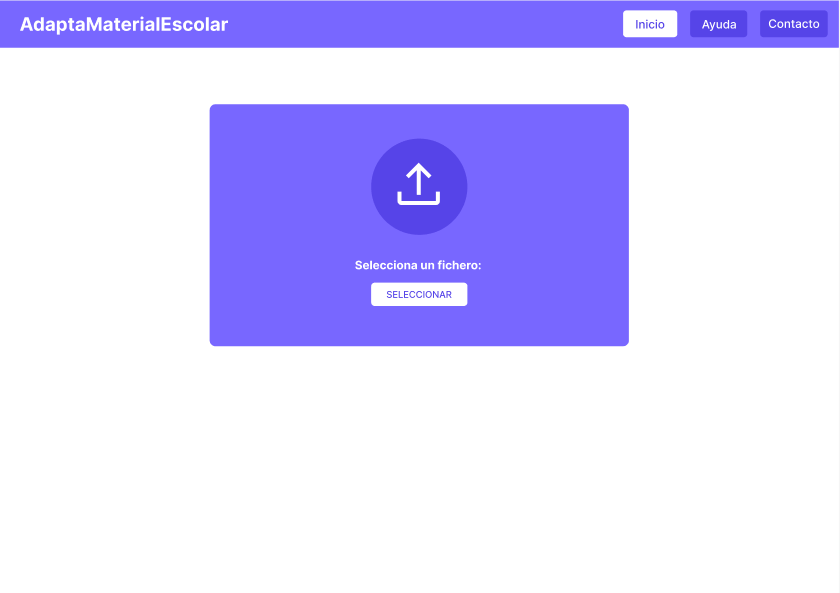
\includegraphics[width=0.6\textwidth]{Diseño/Alberto/PaginaPrincipal1.PNG}
  \caption{Diseño página principal de Alberto.}
  \label{AlbertoPaginaPrincipal1}
\end{figure}

\begin{figure}[ht!]
  \centering
  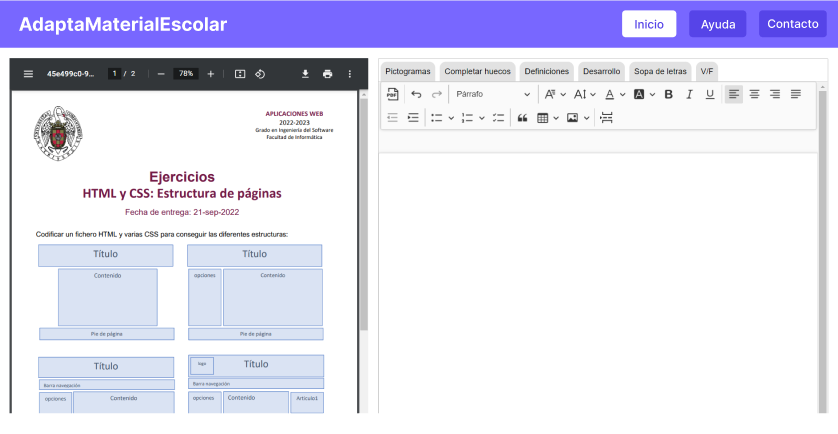
\includegraphics[width=0.6\textwidth]{Diseño/Alberto/PaginaPrincipal2.PNG}
  \caption{Diseño página principal de Alberto.}
  \label{AlbertoPaginaPrincipal2}
\end{figure}


\begin{figure}[ht!]
  \centering
  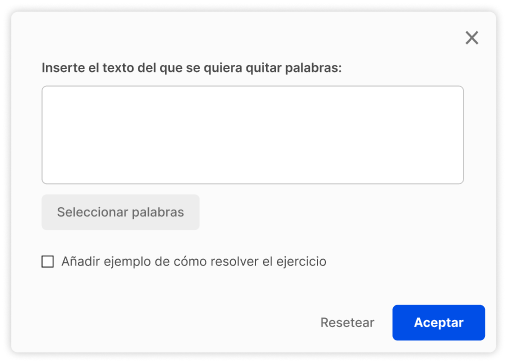
\includegraphics[width=0.6\textwidth]{Diseño/Alberto/Capture13.PNG}
  \caption{Diseño de ejercicios con huecos de Alberto.}
  \label{Alberto13}
\end{figure}

\begin{figure}[ht!]
  \centering
  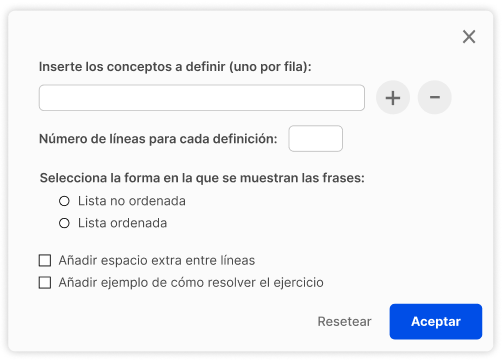
\includegraphics[width=0.6\textwidth]{Diseño/Alberto/Capture14.PNG}
  \caption{Diseño de ejercicios de definiciones de Alberto.}
  \label{Alberto14}
\end{figure}

\begin{figure}[ht!]
  \centering
  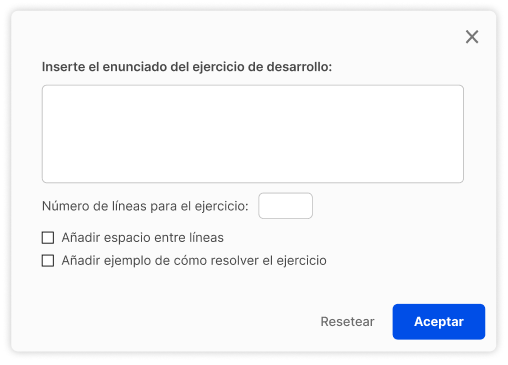
\includegraphics[width=0.6\textwidth]{Diseño/Alberto/Capture15.PNG}
  \caption{Diseño de ejercicios de desarrollo de Alberto.}
  \label{Alberto15}
\end{figure}

\begin{figure}[ht!]
  \centering
  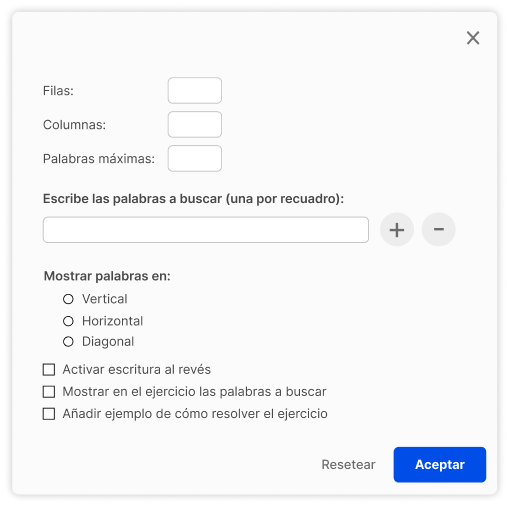
\includegraphics[width=0.6\textwidth]{Diseño/Alberto/Capture16.PNG}
  \caption{Diseño de ejercicios de sopa de letras de Alberto.}
  \label{Alberto16}
\end{figure}

\begin{figure}[ht!]
  \centering
  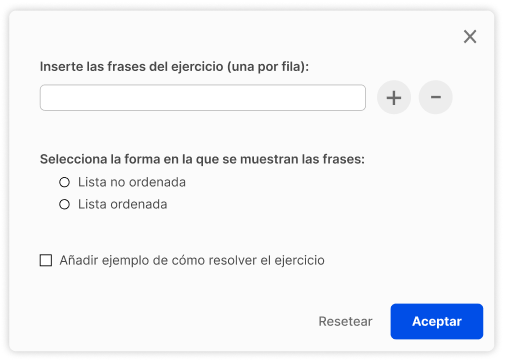
\includegraphics[width=0.6\textwidth]{Diseño/Alberto/Capture17.PNG}
  \caption{Diseño de ejercicios de verdadero y falso de Alberto.}
  \label{Alberto17}
\end{figure}


\begin{figure}[ht!]
  \centering
  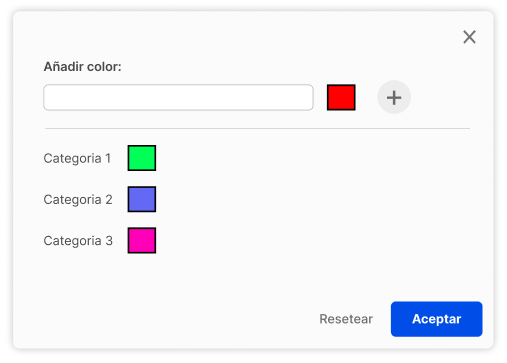
\includegraphics[width=0.6\textwidth]{Diseño/Alberto/Capture01.PNG}
  \caption{Diseño de leyenda de colores de Alberto.}
  \label{Alberto1}
\end{figure}

\begin{figure}[ht!]
  \centering
  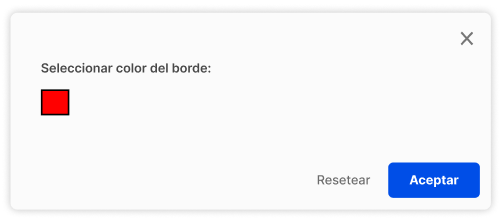
\includegraphics[width=0.6\textwidth]{Diseño/Alberto/Capture02.PNG}
  \caption{Diseño de leyenda de colores por asignatura de Alberto.}
  \label{Alberto2}
\end{figure}

\begin{figure}[ht!]
  \centering
  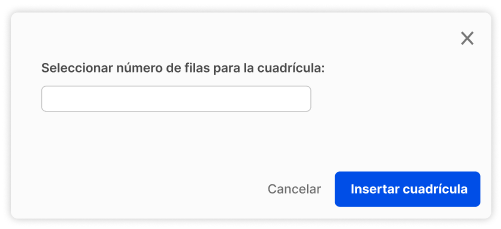
\includegraphics[width=0.6\textwidth]{Diseño/Alberto/Capture03.PNG}
  \caption{Diseño de cuadrícula de Alberto.}
  \label{Alberto3}
\end{figure}

\begin{figure}[ht!]
  \centering
  \includegraphics[width=0.6\textwidth]{Diseño/Alberto/Capture04.PNG}
  \caption{Diseño de doble pauta de Alberto.}
  \label{Alberto4}
\end{figure}

\begin{figure}[ht!]
  \centering
  \includegraphics[width=0.6\textwidth]{Diseño/Alberto/Capture05.PNG}
  \caption{Diseño de ejercicio de flechas de Alberto.}
  \label{Alberto5}
\end{figure}

\begin{figure}[ht!]
  \centering
  \includegraphics[width=0.6\textwidth]{Diseño/Alberto/Capture06.PNG}
  \caption{Diseño de ejercicios de matemáticas con huecos de Alberto.}
  \label{Alberto6}
\end{figure}

\begin{figure}[ht!]
  \centering
  \includegraphics[width=0.6\textwidth]{Diseño/Alberto/Capture08.PNG}
  \caption{Diseño de añadir resumen de Alberto.}
  \label{Alberto8}
\end{figure}

\begin{figure}[ht!]
  \centering
  \includegraphics[width=0.6\textwidth]{Diseño/Alberto/Capture10.PNG}
  \caption{Diseño de pictotraductor de Alberto.}
  \label{Alberto10}
\end{figure}

\begin{figure}[ht!]
  \centering
  \includegraphics[width=0.6\textwidth]{Diseño/Alberto/Capture07.PNG}
  \caption{Diseño de ejercicios de espacios para dibujar de Alberto.}
  \label{Alberto7}
\end{figure}

\begin{figure}[ht!]
  \centering
  \includegraphics[width=0.6\textwidth]{Diseño/Alberto/Capture12.PNG}
  \caption{Diseño de buscar pictogramas de Alberto.}
  \label{Alberto12}
\end{figure}
\chapter{Diseños individuales para la iteración competitiva de Johan Sebastian Salvatierra Gutierrez}
\label{ape:disenyoJohan}

En este apéndice se muestran los diseños individuales realizados por Johan Sebastian Salvatierra Gutierrez para la iteración competitiva. En primer lugar, la Figura \ref{Johan1} donde se puede ver a la izquierda un panel que permite subir un documento, en concreto PDF, en la derecha se encuentra el editor y arriba esta el encabezado con un menú para acceder a las demás pantallas y un botón de ajustes para configurar la pantalla de inicio. En segundo lugar tenemos la Figura \ref{Johan2} donde se encuentra la anterior pantalla pero con todas los ajustes disponibles. En este caso en el lado izquierdo se encuentra dos paneles el panel de arriba es para insertar un documento y el panel de abajo es donde se dispondrá de funciones para la creación de ejercicios. En tercer lugar la Figura \ref{Johan3} muestra qué pasa si se selecciona el menú de navegación. En cuarto lugar, la Figura \ref{Johan4} donde se muestra la pantalla de ``Ayuda'' donde aparecerán diferentes videos para entender el funcionamiento de la aplicación web. En quinto lugar, esta la Figura \ref{Johan5} donde se nos mostrara en formato carta información sobre los integrantes que crearon esta aplicación. Por último, tenemos figuras relacionas con los distintos ejercicios que se proporcionan.

\begin{figure}[ht!]
  \centering
  \includegraphics[width=0.6\textwidth]{Diseño/Johan/Johan1.jpeg}
  \caption{Diseño pantalla de inicio de Johan.}
  \label{Johan1}
\end{figure}

\begin{figure}[ht!]
  \centering
  \includegraphics[width=0.6\textwidth]{Diseño/Johan/Johan2.jpeg}
  \caption{Diseño pantalla de inicio completa de Johan.}
  \label{Johan2}
\end{figure}

\begin{figure}[ht!]
  \centering
  \includegraphics[width=0.6\textwidth]{Diseño/Johan/Johan3.jpeg}
  \caption{Diseño de barra de navegación de Johan.}
  \label{Johan3}
\end{figure}

\begin{figure}[ht!]
  \centering
  \includegraphics[width=0.6\textwidth]{Diseño/Johan/Johan4.jpeg}
  \caption{Diseño de página de información de Johan.}
  \label{Johan4}
\end{figure}

\begin{figure}[ht!]
  \centering
  \includegraphics[width=0.6\textwidth]{Diseño/Johan/Johan5.jpeg}
  \caption{Diseño de página de sobre nosotros de Johan.}
  \label{Johan5}
\end{figure}

\begin{figure}[ht!]
  \centering
  \includegraphics[width=0.6\textwidth]{Diseño/Johan/Johan6}
  \caption{Diseño de sopa de letras.}
  \label{Johan6}
\end{figure}

\begin{figure}[ht!]
  \centering
  \includegraphics[width=0.6\textwidth]{Diseño/Johan/Johan7.jpeg}
  \caption{Diseño de ejercicios de flechas de Johan.}
  \label{Johan7}
\end{figure}

\begin{figure}[ht!]
  \centering
  \includegraphics[width=0.6\textwidth]{Diseño/Johan/Johan8.jpeg}
  \caption{Diseño de leyenda de Johan.}
  \label{Johan8}
\end{figure}

\begin{figure}[ht!]
  \centering
  \includegraphics[width=0.6\textwidth]{Diseño/Johan/Johan9.jpeg}
  \caption{Diseño de leyenda de Johan.}
  \label{Johan9}
\end{figure}
\addtocontents{toc}{\protect\setcounter{tocdepth}{0}}
\chapter{Plan de pruebas: Casos de prueba y guiones de prueba}\label{ape:pruebas}

En este Apéndice se exponen los distintos casos de prueba,  que son escenarios específicos para verificar si la funcionalidad cumple con los requisitos y funcionalidades establecidas, y guiones que se han definido para probar cada funcionalidad de AdaptaMaterialEscolar 2.0.

\section{Funcionalidad de verdadero/falso}
\label{planPruebas:v/f}
A continuación se expone la tabla (Figura \ref{tab:v/f}) con los casos de prueba de la funcionalidad de verdadero/falso y el procedimiento para hacer dichos casos.

\begin{table}[H]
    \resizebox{1.1\textwidth}{!}{
    \begin{tabular}{|c|c|c|c|c|}
    \hline
    \textbf{Precondición} & \textbf{Campo} & \textbf{Condición} & \textbf{Datos de entrada} & \textbf{\begin{tabular}[c]{@{}c@{}}Salida esperada\\ (Postcondición)\end{tabular}} \\ \hline
    Lista={[} {]} & Nueva frase & Longitud de frase \textless{}= 0 & Frase = “” & Lista = {[} {]} \\ \hline
    Lista={[} {]} & Nueva frase & Longitud de frase \textgreater 0 & Frase = “hola” & Lista = {[}“hola” {]} \\ \hline
    Lista={[}“hola”{]} & Editar frase & Longitud de frase \textless{}= 0 y la Frase existe en la lista & Frase = “” & Lista = {[}“hola”{]} \\ \hline
    Lista={[}“hola”{]} & Editar frase & Longitud de frase \textgreater 0 y la Frase existe en la lista & Frase = “adios” & Lista = {[}“adios”{]} \\ \hline
    Lista={[}“hola”{]} & Borrar frase & Existe la frase a borrar en la lista & Frase = “hola” & Lista = {[} {]} \\ \hline
    Lista={[}“hola”, “adios”{]} & Reordenar frases &  & Lista={[}“hola”, “adios”{]} & Lista = {[}“adios”, “hola”{]} \\ \hline
    Lista={[}{]} & Reordenar frases &  & Lista={[}{]} & Lista={[}{]} \\ \hline
    Lista={[}“hola”{]} & Reordenar frases &  & Lista={[}“hola”{]} & Lista={[}“hola”{]} \\ \hline
    \end{tabular}
    }
    \caption{Casos de prueba de la funcionalidad de verdadero/falso.}
    \label{tab:v/f}
\end{table}

\subsection{Procedimiento de prueba}
\label{procedimientoPruebas:v/f}
\begin{enumerate}
    \item Abrir el modal de Verdadero/Falso.
    \item Cerrar el modal.
    \item Abrir el modal de Verdadero/Falso.
    \item Comprobar que no está habilitado el botón de ``Reordenar'' ni el botón de ``O.k''.
    \item No introducir datos al insertar frase y dar click a añadir.
    \item Comprobar que no ha producido ningún cambio.
    \item Introducir datos, ejemplo ``hola''  y dar click a añadir.
    \item Comprobar que se ha introducido en la lista de frases.
    \item Editar la palabra introducida introduciendo una cadena vacía.
    \item Comprobar que no se ha cambiado el valor.
    \item Editar la palabra introducida introduciendo .“adios”.
    \item Comprobar que se ha cambiado el valor al esperado
    \item Darle a borrar la frase.
    \item Comprobar que se ha borrado.
    \item Introducir datos, ejemplo ``pepe'' dar click a añadir.
    \item Comprobar que se ha introducido en la lista de frases.
    \item Comprobar que no está habilitado el botón de reordenar.
    \item Introducir datos, ejemplo ``gato'' y dar click a añadir.
    \item Comprobar que se ha introducido en la lista de frases.
    \item Darle a reordenar .
    \item Comprobar que no tiene el orden anterior.
    \item Darle a ``Ok''.
    \item Comprobar que se ha cerrado el modal.
    \item Abrir el modal de Verdadero/Falso.
    \item Comprobar que los campos están vacíos.
\end{enumerate}

\subsection{Errores encontrados}
\label{errores:v/f}
\begin{itemize}
    \item Editar una palabra hace que se duplique en la lista previa.
    \item Al pulsar el boton de reordenar, puede devolver el mismo orden.
    \item No se reinicia el estado cuando se cierra el modal.
    \item No se puedan editar frases en el documento de trabajo.
\end{itemize}

\section{Funcionalidad de buscar pictograma}
\label{planPruebas:busPicto}
A continuación se expone la tabla (Figura \ref{tab:busPicto}) con los casos de prueba de la funcionalidad de buscar pictograma y el procedimiento para hacer dichos casos.

% Please add the following required packages to your document preamble:
% \usepackage{graphicx}
\begin{table}[H]
    \resizebox{1.1\textwidth}{!}{
    \begin{tabular}{|c|c|c|c|c|}
    \hline
    \textbf{Precondición} & \textbf{Campo} & \textbf{Condición} & \textbf{Datos de entrada} & \textbf{\begin{tabular}[c]{@{}c@{}}Salida esperada\\ (Postcondición)\end{tabular}} \\ \hline
    ListaPicto={[}{]} & Nuevo concepto & Longitud del concepto \textless{}= 0 & concepto= “” & ListaPicto= {[} {]} \\ \hline
    ListaPicto={[}{]} & Nuevo concepto & Longitud del concepto \textgreater 0 & concepto= “hola” & ListaPicto= {[}pictograma1,pictograma2…{]} \\ \hline
    ListaPicto={[}{]} & Nuevo concepto & Longitud del concepto \textgreater 0 & concepto=”jhfueh” & ListaPicto={[}{]}, mensaje=”no se ha encontrado pictograma” \\ \hline
    \end{tabular}
    }
    \caption{Casos de prueba de la funcionalidad de buscar pictograma.}
    \label{tab:busPicto}
\end{table}

\subsection{Procedimiento de prueba}
\label{procedimientoPruebas:busPicto}
\begin{enumerate}
    \item Abrir el modal de Buscar pictograma.
    \item Cerrar el modal.
    \item Abrir el modal de Buscar pictograma.
    \item No introducir concepto y dar click a buscar.
    \item Comprobar que no ha producido ningún cambio.
    \item Introducir un concepto y darle a buscar.
    \item Comprobar que salen los pictogramas relacionados con el concepto.
    \item Darle a un pictograma y comprobar que se ha cerrado el modal.
    \item Abrir el modal de Buscar pictograma.
    \item Comprobar que los campos están vacíos.

\end{enumerate}

\section{Funcionalidad de desarrollo}
\label{planPruebas:desarrollo}
A continuación se expone la tabla (Figura \ref{tab:desarrollo}) con los casos de prueba de la funcionalidad de desarrollo y el procedimiento para hacer dichos casos.

\begin{table}[H]
    \resizebox{1.1\textwidth}{!}{
    \begin{tabular}{|c|c|c|c|c|}
    \hline
    \textbf{Precondición} & \textbf{Campo} & \textbf{Condición} & \textbf{Datos de entrada} & \textbf{\begin{tabular}[c]{@{}c@{}}Salida esperada\\ (Postcondición)\end{tabular}} \\ \hline
    Enunciado=”” & Insertar enunciado & Longitud de enunciado \textless{}= 0 & Enunciado= “” & Enunciado=”” \\ \hline
    Enunciado=”” & Insertar enunciado & Longitud de enunciado \textgreater 0 & Enunciado= “hola” & Enunciado=“hola” \\ \hline
    Enunciado=“hola” & Insertar enunciado & Longitud de enunciado \textless{}= 0 & Enunciado= “” & Enunciado=“” \\ \hline
    Enunciado=“hola” & Insertar enunciado & Longitud de enunciado \textgreater 0 & Enunciado= “adios” & Enunciado= “adios” \\ \hline
    NumeroFilas=1 & Insertar número de filas & Número de filas\textless{}= 0 y existe un enunciado & NumeroFilas= -1 & Enunciado=”” \\ \hline
    NumeroFilas=1 & Insertar número de filas & Número de filas \textgreater 0 y existe un enunciado & NumeroFilas= 2 & Enunciado != “” \\ \hline
    Opción pauta=”” & Elegir pauta & Número de filas \textgreater 0 y existe un enunciado & Opción pauta!= “” & Opción pauta!=”” \\ \hline
    \end{tabular}
    }
    \caption{Casos de prueba de la funcionalidad de desarrollo.}
    \label{tab:desarrollo}
\end{table}

\subsection{Procedimiento de prueba}
\label{procedimientoPruebas:desarrollo}
\begin{enumerate}
    \item Abrir el modal de desarrollo.
    \item Cerrar el modal.
    \item Abrir el modal de desarrollo.
    \item Comprobar que no está habilitado el botón de ``Ok''.
    \item No introducir datos al insertar enunciado y comprobar que no hay nada en la vista previa.
    \item Introducir número de filas mayor que cero y comprobar que no hay nada en la vista previa.
    \item Probar tipos de pauta y comprobar que no hay nada en la vista previa.
    \item Introducir número de filas menor que cero y comprobar que no hay nada en la vista previa.
    \item Probar tipos de pauta y comprobar que no hay nada en la vista previa.
    \item Introducir texto en el insertar enunciado, introducir número de filas mayor que cero y comprobar que se ve en la vista previa .
    \item Probar tipos de pauta y comprobar que se ve en la visa previa.
    \item Probar a cambiar enunciado y comprobar que el cambio se refleja en la vista previa.
    \item Darle a ``Ok''.
    \item Comprobar que se ha cerrado el modal.
    \item Abrir el modal de desarrollo.
    \item Comprobar que los campos están vacíos.
\end{enumerate}

\subsection{Errores encontrados}
\label{errores:desarrollo}
\begin{itemize}
    \item No se debe poder darle a ``Ok'' sin enunciado o con numero de filas $\leq$ 0.
    \item Enunciado con número de filas > 0 provoca un error en consola tras darle ``Ok''.
    \item No debe aparecer pauta si no hay enunciado.
    \item Si se da a la primera opción de pauta no va.
    \item Si el número de filas es un número muy alto como 1000 la página se bloquea.
    \item Al darle a la ``x'' no se resetea.
    \item Boton de ``Ok'' no está desactivado.
    \item  Al añadir la cuadrícula al editable con filas mayor que 1 en la última cuadrícula aparece sin el borde.

\end{itemize}

\section{Funcionalidad de sopa de letras}
\label{planPruebas:sopa}
A continuación se expone la tabla (Figura \ref{tab:sopa}) con los casos de prueba de la funcionalidad de sopa de letras y el procedimiento para hacer dichos casos.

\begin{table}[H]
    \resizebox{1.1\textwidth}{!}{%
    \begin{tabular}{|c|c|c|c|c|}
    \hline
    \textbf{Precondición} & \textbf{Campo} & \textbf{Condición} & \textbf{Datos de entrada} & \textbf{\begin{tabular}[c]{@{}c@{}}Salida esperada\\ (Postcondición)\end{tabular}} \\ \hline
    Listapalabra={[}{]} & Insertar palabra & Longitud de palabra \textless{}= 0 & Palabra= “” & Listapalabra={[}{]} \\ \hline
    Listapalabra={[}{]} & Insertar palabra & Longitud de palabra\textgreater 0 & Palabra= “hola” & Listapalabra={[}“hola”{]} \\ \hline
    Listapalabra={[}“Hola”{]} & Insertar palabra & Longitud de palabra\textless{}= 0 & Palabra= “” & Listapalabra={[}“Hola”{]} \\ \hline
    Listapalabra={[}“Hola”{]} & Insertar palabra & Longitud de palabra\textgreater 0 & palabra= “adios” & Listapalabra={[}“Hola”,”adios”{]} \\ \hline
    Listapalabra={[}“Hola”{]} & Editar palabra & \begin{tabular}[c]{@{}c@{}}Longitud de palabra\textless{}= 0 y \\ la palabra existe en la lista\end{tabular} & palabra= “” & Listapalabra={[}“Hola”{]} \\ \hline
    Listapalabra={[}“Hola”{]} & Editar palabra & \begin{tabular}[c]{@{}c@{}}Longitud de palabra\textgreater 0\\  y la palabra existe en la lista\end{tabular} & palabra= “adios” & Listapalabra= {[}“adios”{]} \\ \hline
    Listapalabra={[}“Hola”{]} & Borrar palabra & Existe la palabra borrar en la lista & palabra= “hola” & Listapalabra= {[} {]} \\ \hline
    NumFilas=1\&\& NumCols=1 & \begin{tabular}[c]{@{}c@{}}Insertar número de\\  filas y columnas\end{tabular} & NumFilas y numCols\textless{}= 0 & \begin{tabular}[c]{@{}c@{}}NumFilas= 0\\ NumCols=0\end{tabular} & NumFilas=1\&\& NumCols=1 \\ \hline
    NumFilas=1\&\& NumCols=1 & \begin{tabular}[c]{@{}c@{}}Insertar número de \\ filas y columnas\end{tabular} & NumFilas y numCols\textgreater 0 \textless 1000 & \begin{tabular}[c]{@{}c@{}}NumFilas= 3\\ NumCols=8\end{tabular} & NumFilas=3 NumCols=8 \\ \hline
    NumFilas=1\&\& NumCols=1 & \begin{tabular}[c]{@{}c@{}}Insertar número de \\ filas y columnas\end{tabular} & NumFilas =1000 numCols=1000 & \begin{tabular}[c]{@{}c@{}}NumFilas= 1000\\ NumCols=1000\end{tabular} & sopa de letras correctamente creada \\ \hline
    \begin{tabular}[c]{@{}c@{}}NumFilas=1\&\& NumCols=1 \&\& \\ Listapalabra={[}“Hola”,”adios”{]} \&\& \\ posicionamiento=horizontal\end{tabular} & \begin{tabular}[c]{@{}c@{}}Insertar número de \\ filas y columnas\end{tabular} & NumFilas\textgreater{}0 numCols\textgreater{}0 & Número de filas=2 numCols=4 & sopa de letras correctamente creada \\ \hline
    \begin{tabular}[c]{@{}c@{}}NumFilas=1\&\& NumCols=1 \&\& \\ Listapalabra={[}“Hola”,”adios”{]} \&\& \\ posicionamiento=horizontal\end{tabular} & \begin{tabular}[c]{@{}c@{}}Insertar número de \\ filas y columnas\end{tabular} & \begin{tabular}[c]{@{}c@{}}NumFilas\textgreater{}0 \&\& \\ 0\textless numCols \\ \textless{}longitud de la palabra más larga\end{tabular} & Número de filas=2 numCols=3 & Error \\ \hline
    \begin{tabular}[c]{@{}c@{}}NumFilas=1\&\& NumCols=1 \&\& \\ Listapalabra={[}“Hola”,”adios”{]} \&\& \\ posicionamiento=vertical\end{tabular} & \begin{tabular}[c]{@{}c@{}}Insertar número de \\ filas y columnas\end{tabular} & \begin{tabular}[c]{@{}c@{}}NumFilas=número de \\ palabras a insertar larga \&\& \\ numCols \textgreater{}0\end{tabular} & Número de filas=2 numCols=4 & sopa de letras correctamente creada \\ \hline
    \begin{tabular}[c]{@{}c@{}}NumFilas=1\&\& NumCols=1 \&\& \\ Listapalabra={[}“Hola”,”adios”{]} \&\& \\ posicionamiento=vertical\end{tabular} & \begin{tabular}[c]{@{}c@{}}Insertar número de \\ filas y columnas\end{tabular} & \begin{tabular}[c]{@{}c@{}}NumFilas\textless{}número de \\ palabras a insertar larga \\ \&\& numCols \textgreater{}0\end{tabular} & Número de filas=1 numCols=4 & Error \\ \hline
    \begin{tabular}[c]{@{}c@{}}NumFilas=1\&\& NumCols=1 \&\& \\ Listapalabra={[}“Hola”,”adios”{]} \&\& \\ posicionamiento=diagonal\end{tabular} & \begin{tabular}[c]{@{}c@{}}Insertar número de \\ filas y columnas\end{tabular} & \begin{tabular}[c]{@{}c@{}}NumFilas=longitud de la \\ palabra más larga\\  larga \&\& numCols=longitud de la \\ palabra más larga\end{tabular} & Número de filas=4 numCols=4 & sopa de letras correctamente creada \\ \hline
    \begin{tabular}[c]{@{}c@{}}NumFilas=1\&\& NumCols=1 \&\& \\ Listapalabra={[}“Hola”,”adios”{]} \&\& \\ posicionamiento=diagonal\end{tabular} & \begin{tabular}[c]{@{}c@{}}Insertar número de \\ filas y columnas\end{tabular} & \begin{tabular}[c]{@{}c@{}}NumFilas\textless{}longitud de la \\ palabra más larga\\  larga \&\& numCols\textless{}longitud de la \\ palabra más larga\end{tabular} & Número de filas=3 numCols=3 & Error \\ \hline
    \end{tabular}%
    }
    \caption{Casos de prueba de la funcionalidad de sopa de letras.}
    \label{tab:sopa}
\end{table}

\subsection{Procedimiento de prueba}
\label{procedimientoPruebas:sopa}
\begin{enumerate}
    \item Abrir el modal de sopa de letras.
    \item Cerrar el modal.
    \item Abrir el modal de sopa de letras.
    \item Comprobar que no está habilitado el botón de ``Ok''.
    \item No introducir datos al insertar las palabras y dar click a añadir.
    \item Comprobar que no ha producido ningún cambio.
    \item Introducir número de filas y columnas mayor que uno.
    \item Comprobar que no ha producido ningún cambio.
    \item Introducir uno o varios posicionamientos de la palabra en la sopa de letras.
    \item Comprobar que no ha producido ningún cambio.
    \item Introducir datos, ejemplo ``pepe''y dar click a añadir.
    \item Comprobar que se ha introducido en la lista de palabras.
    \item Editar palabra introduciendo una cadena vacía.
    \item Comprobar que no ha producido ningún cambio.
    \item Editar palabra introduciendo ``juan''.
    \item Comprobar que la palabra se ha modificado por ``juan''.
    \item Darle a borrar la palabra.
    \item Comprobar que se ha borrado.
    \item Introducir un posicionamiento horizontal e introducir tantas columnas como la longitud de la palabra.
    \item Comprobar que se ha creado la sopa de letras.
    \item Cambia a un posicionamiento vertical e introducir tantas filas como la longitud de la palabra.
    \item Comprobar que se ha creado la sopa de letras.
    \item Cambia a un posicionamiento diagonal e introducir tantas filas y columnas como la longitud de la palabra.
    \item Comprobar que se ha creado la sopa de letras.
    \item Cambia a un posicionamiento al revés e introducir tantas columnas como la longitud de la palabra.
    \item Comprobar que se ha creado la sopa de letras.
    \item Seleccionar todos los tipos de posicionamiento y adecuar el número de columnas y de filas.
    \item Comprobar que se ha creado la sopa de letras.
    \item Darle a ``Ok''.
    \item Comprobar que se ha cerrado el modal.
    \item Abrir el modal de sopa de letras.
    \item Comprobar que los campos están vacíos.
\end{enumerate}

\subsection{Errores encontrados}
\label{errores:sopa}
\begin{itemize}
    \item Si pones 1000 tanto en el número de columnas como en el de filas la pagina no responde.
    \item Al añadir la sopa de letras en el documento de trabajo, posicionar el cursor después del enunciado y dar enter, se crean tantas sopas de letras como veces se da al enter.
    \item Si se ponen 3 números para la filas o las columnas, por ejemplo 300, solo se puede ver los dos primeros números.
\end{itemize}

\section{Funcionalidad de completar huecos}
\label{planPruebas:huecos}
A continuación se expone la tabla (Figura \ref{tab:huecos}) con los casos de prueba de la funcionalidad de completar huecos y el procedimiento para hacer dichos casos.

\begin{table}[H]
    \resizebox{1.1\textwidth}{!}{
    \begin{tabular}{|c|c|c|c|c|}
    \hline
    \textbf{Precondición} & \textbf{Campo} & \textbf{Condición} & \textbf{Datos de entrada} & \textbf{\begin{tabular}[c]{@{}c@{}}Salida esperada\\ (Postcondición)\end{tabular}} \\ \hline
    Texto=”” & Nuevo texto & Longitud de texto\textless{}= 0 & Texto= “” & Texto= “” \\ \hline
    Texto=”” & Nuevo texto & Longitud de texto\textgreater 0 & Texto= “hola” & Texto=“hola” \\ \hline
    Texto =”” & Introducir huecos & Longitud de texto\textless{}= 0 & \begin{tabular}[c]{@{}c@{}}Tamaño de hueco \\ que pertenece \\ a algún tamaño de \\ hueco disponible\end{tabular} & Texto=”” \\ \hline
    Texto =”Hola esto es una prueba” & Introducir huecos & \begin{tabular}[c]{@{}c@{}}Longitud de texto\textgreater 0\\  y el hueco no \\ sea un espacio\end{tabular} & \begin{tabular}[c]{@{}c@{}}Tamaño de hueco \\ que pertenece \\ a algún tamaño de \\ hueco disponible\end{tabular} & Texto =”\_\_\_\_\_\_\_ esto es una \_\_\_\_\_\_\_” \\ \hline
    Texto =”Hola esto es una prueba” & Editar Texto & Longitud de texto\textgreater 0 & Texto =”Adiós esto es una prueba”” & Texto =”Adiós esto es una prueba”” \\ \hline
    \end{tabular}
    }
    \caption{Casos de prueba de la funcionalidad de completar huecos.}
    \label{tab:huecos}
\end{table}

\subsection{Procedimiento de prueba}
\label{procedimientoPruebas:huecos}
\begin{enumerate}
    \item Abrir el modal de completar huecos.
    \item Cerrar el modal.
    \item Abrir el modal de completar huecos.
    \item Comprobar que sin texto introducido no se puede darle a ``Ok''.
    \item Comprobar que sin texto introducido no se puede darle a añadir huecos.
    \item Insertar texto como por ejemplo ``Hola esto es una prueba'' comprobar que se puede dar click al botón de añadir hueco.
    \item Borrar texto y ver como no se puede darle a ok y no se puede darle a añadir huecos.
    \item Insertar texto como por ejemplo ``Hola esto es una prueba'' comprobar que se puede dar click al botón de añadir hueco.
    \item Dar click al botón de añadir hueco y probar todos los tipos de añadir hueco.
    \item Probar a dar click al boton de editar texto e introducir por ejemplo ``Adiós esto es una prueba''.
    \item Dar click al botón de añadir hueco y probar todos los tipos de añadir hueco.
    \item Comprobar que no puedes convertir los espacios en huecos.
    \item Dar click al ``Ok''.
    \item Comprobar que se ha cerrado el modal.
    \item Abrir el modal de completar huecos.
    \item Comprobar que los campos están vacíos.
\end{enumerate}

\subsection{Errores encontrados}
\label{errores:huecos}
\begin{itemize}
    \item Permite convertir los espacios en huecos.
    \item Si hay una palabra con tilde no te crea bien el hueco.
\end{itemize}

\section{Funcionalidad de definiciones}
\label{planPruebas:definiciones}
A continuación se expone la tabla (Figura \ref{tab:definiciones}) con los casos de prueba de la funcionalidad de definiciones y el procedimiento para hacer dichos casos.

\begin{table}[H]
    \resizebox{1.1\textwidth}{!}{
    \begin{tabular}{|c|c|c|c|c|}
    \hline
    \textbf{Precondición} & \textbf{Campo} & \textbf{Condición} & \textbf{Datos de entrada} & \textbf{\begin{tabular}[c]{@{}c@{}}Salida esperada\\ (Postcondición)\end{tabular}} \\ \hline
    Lista={[} {]} & Nueva definición & Longitud de frase \textless{}= 0 & Frase = “” & Lista = {[} {]} \\ \hline
    Lista={[} {]} & Nueva definición & Longitud de frase \textgreater 0 & Frase = “hola” & Lista = {[}“hola” {]} \\ \hline
    Lista={[}“hola”{]} & Editar definición & Longitud de frase \textless{}= 0 y la Frase existe en la lista & Frase = “” & Lista = {[}“hola”{]} \\ \hline
    Lista={[}“hola”{]} & Editar definición & \begin{tabular}[c]{@{}c@{}}Longitud de frase \textgreater 0\\  y la Frase existe en la lista\end{tabular} & Frase = “adios” & Lista = {[}“adios”{]} \\ \hline
    Lista={[}“hola”{]} & Borrar definición & Existe la frase a borrar en la lista & Frase = “hola” & Lista = {[} {]} \\ \hline
    NumeroFilas=1 & Insertar número de filas & Número de filas\textless{}= 0 y existe un enunciado & NumeroFilas= -1 & Enunciado=”” \\ \hline
    NumeroFilas=1 & Insertar número de filas & Número de filas \textgreater 0 y existe un enunciado & NumeroFilas= 2 & Enunciado != “” \\ \hline
    Opción pauta=”” & Elegir pauta & Número de filas \textgreater 0 y existe un enunciado & Opción pauta!= “” & Opción pauta!=”” \\ \hline
    \end{tabular}
    }
    \caption{Casos de prueba de la funcionalidad de definiciones.}
    \label{tab:definiciones}
\end{table}

\subsection{Procedimiento de prueba}
\label{procedimientoPruebas:definiciones}
\begin{enumerate}
    \item Abrir el modal de definiciones.
    \item Cerrar el modal.
    \item Abrir el modal de definiciones.
    \item Intentar darle al botón de ``Ok'' y comprobar que no está habilitado.
    \item No introducir datos al insertar definición y dar click a añadir.
    \item Comprobar que no se ha producido ningún cambio.
    \item Introducir datos, ejemplo ``hola'' y dar click a añadir.
    \item Comprobar que se ha introducido en la lista de frases.
    \item Editar palabra introducida escribiendo una cadena vacía.
    \item Comprobar que no se ha cambiado el valor.
    \item Editar la palabra introducida escribiendo ``adios''.
    \item Comprobar que se ha cambiado el valor al esperado.
    \item Darle a borrar la definición.
    \item Comprobar que se ha borrado.
    \item Introducir datos, ejemplo ``pepe'' y dar click a añadir.
    \item Comprobar que se ha introducido en la lista de definiciones.
    \item Introducir un número de filas menor o igual que cero y comprobar que no se dibujan en la vista previa.
    \item Introducir un número de filas mayor que 100 y comprobar que no se dibujan en la vista previa.
    \item Introducir un número de filas mayor que cero pero menor o igual que 100 y comprobar que se dibuja el número indicado de filas.
    \item Probar todos los tipos de pautas y comprobar que se dibuja el tipo de pauta indicado en cada caso.
    \item Darle a ``Ok''.
    \item Comprobar que se ha cerrado el modal y se ha añadido el ejercicio al editable.
    \item Abrir el modal de definiciones.
    \item Comprobar que los campos están vacíos.
\end{enumerate}

\subsection{Errores encontrados}
\label{errores:definicion}
\begin{itemize}
    \item Se puede insertar el ejercicio en el editor sin ninguna definición.
    \item Se puede insertar un número negativo de filas.
    \item Se pueden añadir definiciones que sean solamente espacios.
    \item Al darle a la ``x'' no se resetea.
\end{itemize}


\section{Funcionalidad de generar resumen}
\label{planPruebas:resumen}
A continuación se expone la tabla (Figura \ref{tab:resumen}) con los casos de prueba de la funcionalidad de generar resumen y el procedimiento para hacer dichos casos.

\begin{table}[H]
    \resizebox{1.1\textwidth}{!}{%
    \begin{tabular}{|c|c|c|c|c|}
    \hline
    \textbf{Precondición} & \textbf{Campo} & \textbf{Condición} & \textbf{Datos de entrada} & \textbf{\begin{tabular}[c]{@{}c@{}}Salida esperada\\ (Postcondición)\end{tabular}} \\ \hline
    TextoResumido=”” & Texto Original & Longitud del TextoOriginal\textless{}= 0 & TextoOriginal= “” & TextoResumido=”” \\ \hline
    TextoResumido=”” & Texto Original & Longitud del TextoOriginal\textgreater 0 & TextoOriginal= “...” & \begin{tabular}[c]{@{}c@{}}TextoResumido=”...”\\ siendo Longitud del TextoResumido \\ \textless Longitud del TextoOriginal\end{tabular} \\ \hline
    TextoResumido=”” & Texto Original & Longitud del TextoOriginal\textgreater 0 & TextoOriginal= “dgsgds” & TextoResumido=”” \\ \hline
    TextoResumido=”” & Tamaño & Tamaño \textless{}= 0 & TextoOriginal= “...” & TextoResumido=”” \\ \hline
    TextoResumido=”” & Tamaño & Tamaño \textgreater 0 & TextoOriginal= “...” y Tamaño=10 & \begin{tabular}[c]{@{}c@{}}TextoResumido=”...” \\ con longitud de TextoResumido  = 10\end{tabular} \\ \hline
    \end{tabular}%
    }
    \caption{Casos de prueba de la funcionalidad de generar resumen.}
    \label{tab:resumen}
\end{table}



\subsection{Procedimiento de prueba}
\label{procedimientoPruebas:resumen}
\begin{enumerate}
    \item Abrir el modal de Generar Resumen.
    \item Cerrar el modal.
    \item Abrir el modal de Generar Resumen.
    \item No introducir texto original y dar click a resumir.
    \item Comprobar que no ha producido ningún cambio.
    \item Introducir un texto, elegir una cantidad de palabras menor o igual que cero y darle a resumir.
    \item Cerrar el modal.
    \item Abrir el modal de Generar Resumen.
    \item Comprobar que se ha reseteado el modal.
    \item Introducir un texto, elegir una cantidad de palabras menor o igual que cero y darle a resumir.
    \item Comprobar que no ha producido ningún cambio.
    \item Introducir un texto, elegir una cantidad de palabras mayor que cero y darle a resumir.
    \item Comprobar que se ha devuelto lo especificado.
    \item Comprobar que los campos están vacíos.
    \item Introducir un texto no coherente, elegir una cantidad de palabras mayor que cero y darle a resumir.
    \item Comprobar que no ha producido ningún cambio.

\end{enumerate}

\subsection{Errores encontrados}
\label{errores:resumen}
\begin{itemize}
    \item Plantear no permitir elegir 0 palabras es una opción que nunca se podría dar.
    \item Cuando se introduce caractares sin sentido al resumirlo se produce un resultados como los siguiente: ``No se ha podido resumir'', no tiene sentido. Esto no debería poder introducirse en el editor
\end{itemize}

\section{Funcionalidad de leyenda de colores}
\label{planPruebas:leyenda}
A continuación se expone la tabla (Figura \ref{tab:leyenda}) con los casos de prueba de la funcionalidad de leyenda de colores y el procedimiento para hacer dichos casos.

\begin{table}[H]
    \resizebox{1.1\textwidth}{!}{
    \begin{tabular}{|c|c|c|c|c|}
    \hline
    \textbf{Precondición} & \textbf{Campo} & \textbf{Condición} & \textbf{Datos de entrada} & \textbf{\begin{tabular}[c]{@{}c@{}}Salida esperada\\ (Postcondición)\end{tabular}} \\ \hline
    Lista={[} {]} & Nuevo concepto & Longitud de frase \textless{}= 0 & Frase = “” & Lista = {[} {]} \\ \hline
    Lista={[} {]} & Nuevo concepto & Longitud de frase \textgreater 0 & Frase = “hola” & Lista = {[}“hola”(0,0,0) {]} \\ \hline
    Lista={[}“hola”(0,0,0){]} & Editar concepto & Longitud de frase \textless{}= 0 y la Frase existe en la lista & Frase = “” & Lista = {[}“hola”(0,0,0){]} \\ \hline
    Lista={[}“hola”(0,0,0){]} & Editar concepto & \begin{tabular}[c]{@{}c@{}}Longitud de frase \textgreater 0\\  y la Frase existe en la lista\end{tabular} & Frase = “adios” & Lista = {[}“adios”(0,0,0,){]} \\ \hline
    Lista={[}“hola”(0,0,0){]} & Editar color & \begin{tabular}[c]{@{}c@{}}Color válido\\  y la Frase existe en la lista\end{tabular} & Color = (255,0,0) & Lista = {[}“hola”(255,0,0,){]} \\ \hline
    Lista={[}“hola”(0,0,0){]} & Borrar concepto & Existe la frase a borrar en la lista & Frase = “hola” & Lista = {[} {]} \\ \hline
    \end{tabular}
    }
    \caption{Casos de prueba de la funcionalidad de leyenda de colores.}
    \label{tab:leyenda}
\end{table}

\subsection{Procedimiento de prueba}
\label{procedimientoPruebas:leyenda}
\begin{enumerate}
    \item Abrir el modal.
    \item Cerrar el modal.
    \item Abrir el modal otra vez.
    \item Intentar darle al botón de ``Ok'' y comprobar que no está habilitado.
    \item No introducir datos al insertar un concepto y dar click a añadir.
    \item Comprobar que no se ha producido ningún cambio.
    \item Introducir datos, ejemplo ``hola'' y dar click a añadir.
    \item Comprobar que se ha introducido en la lista de conceptos.
    \item Editar palabra introducida escribiendo una cadena vacía.
    \item Comprobar que no se ha cambiado el valor.
    \item Editar la palabra introducida escribiendo ``adios''.
    \item Comprobar que se ha cambiado el valor al esperado.
    \item Editar el color seleccionado un color diferente.
    \item Comprobar que se ha cambiado el color.
    \item Darle a borrar el concepto.
    \item Comprobar que se ha borrado.
    \item Introducir datos, ejemplo ``pepe'' y dar click a añadir.
    \item Comprobar que se ha introducido en la lista de definiciones.
    \item Darle a ``Ok''.
    \item Comprobar que se ha cerrado el modal y se ha añadido la leyenda al editable.
    \item Abrir el modal.
    \item Comprobar que los campos están vacíos.
\end{enumerate}

\subsection{Errores encontrados}
\label{errores:leyenda}
\begin{itemize}
    \item  Se puede editar y añadir solamente espacios.
    \item  Al darle a la ``x'' no se resetea.
    \item Si se añade una palabra demasiado larga, no queda espacio para el cuadro del color.
\end{itemize}

\section{Funcionalidad de espacios para dibujar}
\label{planPruebas:dibujar}
A continuación se expone la tabla (Figura \ref{tab:dibujar}) con los casos de prueba de la funcionalidad de espacios para dibujar y el procedimiento para hacer dichos casos.

\begin{table}[H]
    \resizebox{1.1\textwidth}{!}{
    \begin{tabular}{|c|c|c|c|c|}
    \hline
    \textbf{Precondición} & \textbf{Campo} & \textbf{Condición} & \textbf{Datos de entrada} & \textbf{\begin{tabular}[c]{@{}c@{}}Salida esperada\\ (Postcondición)\end{tabular}} \\ \hline
    Enunciado=”” & Insertar enunciado & Longitud de enunciado\textless{}= 0 & Enunciado= “” & Enunciado=”” \\ \hline
    Enunciado=”” & Insertar enunciado & Longitud de enunciado\textgreater 0 & Enunciado= “hola” & Enunciado=“hola” \\ \hline
    Enunciado=“hola” & Insertar enunciado & Longitud de enunciado\textless{}= 0 & Enunciado= “” & Enunciado=“” \\ \hline
    Enunciado=“hola” & Insertar enunciado & Longitud de enunciado\textgreater 0 & Enunciado= “adios” & Enunciado= “adios” \\ \hline
    espacio=1 & Insertar espacio & espacio\textless{}= 0 y existe un enunciado & espacio= -1 & Enunciado=”” \\ \hline
    espacio=1 & Insertar espacio & espacio \textgreater 0 y existe un enunciado & espacio= 2 & Enunciado != “” \\ \hline
    \end{tabular}
    }
    \caption{Casos de prueba de la funcionalidad de espacios para dibujar.}
    \label{tab:dibujar}
\end{table}

\subsection{Procedimiento de prueba}
\label{procedimientoPruebas:dibujar}
\begin{enumerate}
    \item Abrir el modal de espacios para dibujar.
    \item Cerrar el modal.
    \item Abrir el modal de espacios para dibujar.
    \item Comprobar que no está habilitado el botón de ``Ok''.
    \item No introducir datos al insertar enunciado y comprobar que no hay nada en la vista previa.
    \item Introducir espacio mayor que cero y comprobar que no hay nada en la vista previa.
    \item Introducir espacio menor que cero y comprobar que no hay nada en la vista previa.
    \item Introducir texto en el insertar enunciado, introducir espacio  mayor que cero y comprobar que se ve en la vista previa.
    \item Probar a cambiar enunciado y comprobar que el cambio se refleja en la vista previa.
    \item Desmarcar recuadro y ver en vista previa que no hay recuadro.
    \item Marcar recuadro y ver que aparece en vista previa.
    \item Darle a ``Ok''.
    \item Comprobar que se ha cerrado el modal.
    \item Abrir el modal de  espacios para dibujar.
    \item Comprobar que los campos están vacíos.
\end{enumerate}

\subsection{Errores encontrados}
\label{errores:espacio}
\begin{itemize}
    \item  Como nombre del modal tienes puesto Ejercicios de desarollo, sería Ejercicios para dibujar.
    \item No funciona el recuadrar, si lo marcas y luego lo desmarcas en la vista previa no se refleja.
\end{itemize}

\section{Funcionalidad de pictotraductor}
\label{planPruebas:pictotraductor}
A continuación se expone la tabla (Figura \ref{tab:pictotraductor}) con los casos de prueba de la funcionalidad de pictotraductor y el procedimiento para hacer dichos casos.

\begin{table}[H]
    \resizebox{1.1\textwidth}{!}{
    \begin{tabular}{|l|l|l|l|l|}
    \hline
    \textbf{Precondición} & \textbf{Campo} & \textbf{Condición} & \textbf{Datos de entrada} & \textbf{\begin{tabular}[c]{@{}l@{}}Salida esperada\\ (Postcondición)\end{tabular}} \\ \hline
    TextoOriginal=”” & Insertar texto & Longitud de texto\textless{}= 0 & texto= “” & TextoOriginal=”” \\ \hline
    TextoOriginal=”” & Insertar texto & Longitud de texto\textgreater 0 & texto= “La libélula tiene cuatro alas” & \begin{tabular}[c]{@{}l@{}}TextoOriginal=\\ “La libélula tiene cuatro alas””\end{tabular} \\ \hline
    \begin{tabular}[c]{@{}l@{}}TextoOriginal=\\ “La libélula tiene cuatro alas”\end{tabular} & Insertar texto & Longitud de texto\textless{}= 0 & texto= “” & TextoOriginal=“” \\ \hline
    \begin{tabular}[c]{@{}l@{}}TextoOriginal=\\ “La libélula tiene cuatro alas”\end{tabular} & Insertar texto & Longitud de texto\textgreater 0 & \begin{tabular}[c]{@{}l@{}}texto= \\ “descomponer los alimentos para obtener sus nutrientes”\end{tabular} & \begin{tabular}[c]{@{}l@{}}TextoOriginal= \\ “descomponer los alimentos para obtener sus nutrientes”\end{tabular} \\ \hline
    \begin{tabular}[c]{@{}l@{}}TextoOriginal=\\ “La libélula tiene cuatro alas”\end{tabular} & opciones de texto & Longitud de texto\textgreater 0 & opciones de texto=arriba & \begin{tabular}[c]{@{}l@{}}Pictogramas con texto \\ encima del pictograma\end{tabular} \\ \hline
    \begin{tabular}[c]{@{}l@{}}TextoOriginal=\\ “La libélula tiene cuatro alas”\end{tabular} & opciones de texto & Longitud de texto\textgreater 0 & opciones de texto=debajo & \begin{tabular}[c]{@{}l@{}}Pictogramas con texto \\ debajo del pictograma\end{tabular} \\ \hline
    \begin{tabular}[c]{@{}l@{}}TextoOriginal=\\ “La libélula tiene cuatro alas”\end{tabular} & opciones de texto & Longitud de texto\textgreater 0 & opciones de texto=sin texto & Pictogramas sin texto \\ \hline
    \begin{tabular}[c]{@{}l@{}}TextoOriginal=\\ “La libélula tiene cuatro alas\end{tabular} & opciones de color & Longitud de texto\textgreater 0 & opciones de color=blanco y negro & Pictograma en blanco y negro \\ \hline
    \begin{tabular}[c]{@{}l@{}}TextoOriginal=\\ “La libélula tiene cuatro alas”\end{tabular} & vista picto & Longitud de texto\textgreater 0 & visualización de un  picto oculta & Pictograma oculto \\ \hline
    \begin{tabular}[c]{@{}l@{}}TextoOriginal=\\ “La libélula tiene cuatro alas”\end{tabular} & vista picto & Longitud de texto\textgreater 0 & visualización de todos los  picto oculta & boton Ok deshabilitado \\ \hline
    \end{tabular}
    }
    \caption{Casos de prueba de la funcionalidad pictotraductor.}
    \label{tab:pictotraductor}
\end{table}

\subsection{Procedimiento de prueba}
\label{procedimientoPruebas:pictotraductor}
\begin{enumerate}
    \item Abrir el modal de pictotraductor.
    \item Cerrar el modal.
    \item Abrir el modal de pictotraductor.
    \item Comprobar que no está habilitado el botón de ``Ok''.
    \item No introducir datos al insertar enunciado y comprobar que no hay nada en la vista previa.
    \item Introducir cadena vacía y comprobar que no hay nada en la vista previa
    \item Introducir ``La libélula tiene cuatro alas'' y comprobar que aparecen los respectivos pictogramas.
    \item Introducir ``La libélula tiene cuatro alas'' y comprobar que aparecen los respectivos pictogramas y cambiar el texto por ``descomponer los alimentos''. para obtener sus nutrientes y ver que los pictogramas se han creado.
    \item Introducir ``La libélula tiene cuatro alas'', poner como opción de texto arriba y comprobar que aparecen los pictogramas con el texto arriba.
    \item Introducir ``La libélula tiene cuatro alas'', poner como opción de texto debajo y comprobar que aparecen los pictogramas con el texto debajo.
    \item Introducir ``La libélula tiene cuatro alas'', poner como opción de texto sin texto y comprobar que aparecen los pictogramas sin texto.
    \item Introducir ``La libélula tiene cuatro alas'', poner como opción de color blanco y negro  y comprobar que aparecen los pictogramas en blanco y negro.
    \item Introducir ``La libélula tiene cuatro alas'', comprobar que aparecen los pictogramas y ocultar uno.
    \item Introducir ``La libélula tiene cuatro alas'', comprobar que aparecen los pictogramas y ocultar todos, ver que el botón de ``Ok'' no está habilitado.
    \item Darle a ``Ok''.
    \item Comprobar que se ha cerrado el modal.
    \item Abrir el modal de  pictotraductor.
    \item Comprobar que los campos están vacíos.
\end{enumerate}

\subsection{Errores encontrados}
\label{errores:pictotra}
\begin{itemize}
    \item Cuando escribes una frase y una de las palabras no tiene pictograma en el editable se muestra un cuadrado donde pone la palabra y el icono que sale cuando no ha cargado la imagen..
    \item Cuando ocultas todos los pictogramas no deberia estar habilitado el botón de ``OK''.
    \item  Cuando quieres editar algo que ya esta en el editable la configuración está mal.
    \item Si pones algo que no existe (djfhwjhfb) se habilita el botón de ``Ok'' y al darle pasa lo mismo que en el primer punto.
    \item  Si pongo espacios se habilita el botón de pictotraductor.
\end{itemize}


\section{Funcionalidad de relacionar conceptos}
\label{planPruebas:conceptos}
A continuación se expone la tabla (Figura \ref{tab:conceptos}) con los casos de prueba de la funcionalidad de relacionar conceptos y el procedimiento para hacer dichos casos.

\begin{table}[H]
    \resizebox{1.1\textwidth}{!}{
    \begin{tabular}{|c|c|c|c|c|}
    \hline
    \textbf{Precondición} & \textbf{Campo} & \textbf{Condición} & \textbf{Datos de entrada} & \textbf{\begin{tabular}[c]{@{}c@{}}Salida esperada\\ (Postcondición)\end{tabular}} \\ \hline
    NumFilas=0 y NumCols=0 & Insertar filas y columnas & NumFilas\textless{}= 1 y NumCols\textless{}= 1 & NumFilas=0 y NumCols=0 & La tabla de conceptos no sale \\ \hline
    NumFilas=0 y NumCols=0 & Insertar filas y columnas & \begin{tabular}[c]{@{}c@{}}1 \textless NumFilas \textless 20 \\ y 1 \textless NumCols\textless 20\end{tabular} & NumFilas=2 y NumCols=2 & Dos columnas con dos filas \\ \hline
    NumFilas=2 y NumCols=2 & Insertar filas y columnas & \begin{tabular}[c]{@{}c@{}}1 \textless NumFilas \textless 20 \\ y 1 \textless NumCols\textless 20\end{tabular} & \begin{tabular}[c]{@{}c@{}}En la tabla añadir: \\ “animales”, “vaca”, “gato”\end{tabular} & Tabla con esos datos \\ \hline
    NumFilas=2 y NumCols=2 & Insertar filas y columnas & \begin{tabular}[c]{@{}c@{}}1 \textless NumFilas \textless 20 \\ y 1 \textless NumCols\textless 20\end{tabular} & En la tabla añadir cadenas vacías & Botón de Ok deshabilitado \\ \hline
    \begin{tabular}[c]{@{}c@{}}En una columna: “animales”, \\ en otra: “gato”, “vaca” y NumFilas=2 y NumCols=2\end{tabular} & Reordenar &  & \begin{tabular}[c]{@{}c@{}}En la tabla: \\ “animales”, “vaca”, “gato”\end{tabular} & \begin{tabular}[c]{@{}c@{}}En una columna: \\ “animales”, en otra: “gato”, “vaca”\end{tabular} \\ \hline
    Tabla vacía & Reordenar &  & Tabla vacía & Tabla vacía \\ \hline
    \end{tabular}
    }
    \caption{Casos de prueba de la funcionalidad de relacionar conceptos.}
    \label{tab:conceptos}
\end{table}



\subsection{Procedimiento de prueba}
\label{procedimientoPruebas:conceptos}
\begin{enumerate}
    \item Abrir el modal de relacionar conceptos.
    \item Cerrar el modal.
    \item Abrir el modal de relacionar conceptos.
    \item Comprobar que no está habilitado el botón de ``Ok''.
    \item Introducir número de columnas y filas  menores a 1.
    \item Comprobar que las columnas y filas no aparecen.
    \item Introducir número de columnas y filas mayores que 1.
    \item Comprobar que ese número de  las columnas y filas aparecen como tabla dividida en columnas.
    \item Introducir texto en las celdas.
    \item Ver que aparece en la vista previa.
    \item Reordenar y ver que se desordenan.
    \item Eliminar los concepto puestos en las celdas
    \item Poner en las celdas espacios en blanco
    \item Ver que el botón de ``Ok'' está deshabilitado
    \item Volver a poner conceptos en las celdas
    \item Darle a ``Ok''.
    \item Comprobar que se ha cerrado el modal.
    \item Abrir el modal de relacionar conceptos.
    \item Comprobar que los campos están vacíos.

\end{enumerate}


\subsection{Errores encontrados}
\label{errores:pictotra}
\begin{itemize}
    \item No deja borrar la palabra entera, siempre se queda la ultima letra.
    \item Cuando creas una tabla de las dimensiones que sea y escribes dos conceptos en la misma columna se activa reordenar y el botón de ``Ok''.
    \item  Si en una celda pongo espacios me lo da como bueno.

\end{itemize}

\section{Funcionalidad de ejercicios de matemáticas}\label{planPruebas:mates}
A continuación se expone la tabla (Figura \ref{tab:mate}) con los casos de prueba de la funcionalidad de ejercicios de matemáticas y el procedimiento para hacer dichos casos.

\begin{table}[H]
    \resizebox{1.1\textwidth}{!}{
    \begin{tabular}{|c|c|c|c|c|}
    \hline
    \textbf{Precondición} & \textbf{Campo} & \textbf{Condición} & \textbf{Datos de entrada} & \textbf{\begin{tabular}[c]{@{}c@{}}Salida esperada\\ (Postcondición)\end{tabular}} \\ \hline
     & Insertar hueco (tecla espacio) &  &  & \begin{tabular}[c]{@{}c@{}}Se ha insertado un nuevo hueco, \\ justo después del hueco seleccionado.\end{tabular} \\ \hline
    1 hueco y 1 fórmula & \begin{tabular}[c]{@{}c@{}}Borrar hueco\\ (tecla retroceso)\end{tabular} &  &  & \begin{tabular}[c]{@{}c@{}}Se ha mantenido el hueco, ya que como mínimo \\ debe haber un hueco y una fórmula.\end{tabular} \\ \hline
    Al menos 2 huecos & \begin{tabular}[c]{@{}c@{}}Borrar hueco\\ (tecla retroceso)\end{tabular} &  &  & Se ha borrado el hueco seleccionado. \\ \hline
     & Insertar fórmula (tecla enter) &  &  & \begin{tabular}[c]{@{}c@{}}Se ha insertado una nueva formula, \\ justo debajo de la fórmula seleccionada.\end{tabular} \\ \hline
    \begin{tabular}[c]{@{}c@{}}Al menos dos fórmulas y \\ solo un hueco en cada una\end{tabular} & \begin{tabular}[c]{@{}c@{}}Borrar hueco\\ (tecla retroceso)\end{tabular} &  &  & Se ha borrado la fórmula del hueco seleccionado. \\ \hline
     & Huecos &  & “1+ =2” & Fórmula = “1 + \_\_\_ = 2” \\ \hline
    \end{tabular}
    }
    \caption{Casos de prueba de la funcionalidad de ejercicios de matemáticas.}
    \label{tab:mate}
\end{table}

\subsection{Procedimiento de prueba}
\label{procedimientoPruebas:mate}
\begin{enumerate}
    \item Abrir el modal de Fórmula matemática.
    \item Comprobar que se ha abierto el modal.
    \item Cerrar el modal.
    \item Comprobar que se ha cerrado el modal.
    \item Abrir el modal de Fórmula matemática.
    \item Comprobar que no está habilitado el botón de ``Ok''.
    \item Introducir datos en el primer hueco, ejemplo ``123''.
    \item Comprobar que se ha habilitado el botón de ``Ok''.
    \item Pulsar el botón de ``Ok''.
    \item Comprobar que se ha cerrado el modal y se ha introducido el texto correctamente en el documento de trabajo.
    \item Abrir el modal de Fórmula matemática.
    \item Pulsar espacio varias veces (Probar manteniendo pulsado el espacio también).
    \item Comprobar que se han creado nuevos huecos y que el cursor está en la última posición.
    \item Pulsar la tecla de retroceso varias veces (Probar manteniendo pulsada la tecla de retroceso también).
    \item Comprobar que se han borrado huecos y que el cursor está en la misma posición.
    \item Escribir una fórmula con huecos, por ejemplo`` 2 + \rule{10mm}{0.1mm} = 5''.
    \item Pulsar el botón de ``Ok''.
    \item Comprobar que se ha cerrado el modal y se ha introducido correctamente el texto en el documento de trabajo.
    \item Introducir datos, ejemplo ``123''.
    \item Añadir varios huecos.
    \item Cerrar el modal.
    \item Abrir el modal de Fórmula matemática.
    \item Comprobar que los campos están vacíos.
\end{enumerate}

\subsection{Errores encontrados}
\label{errores:mates}
\begin{itemize}
    \item Cuando no se ha introducido ningún valor, el botón de Ok no se muestra como si estuviera desactivado, aunque sí que está desactivado ya que no se puede introducir una formula vacía.
    \item Si mantienes el espacio pulsado, se crean huecos más rápido que el movimiento del cursor, entonces el cursor no acaba en la última posición, aunque hubiese empezado en la última posición.
\end{itemize}

\section{Funcionalidad de exportar a PDF}
\label{planPruebas:exportar}
A continuación se expone la tabla (Figura \ref{tab:exportar}) con los casos de prueba de la funcionalidad de exportar a PDF y el procedimiento para hacer dichos casos.

\begin{table}[H]
    \resizebox{1.1\textwidth}{!}{
    \begin{tabular}{|c|c|c|c|c|}
    \hline
    \textbf{Precondición} & \textbf{Campo} & \textbf{Condición} & \textbf{Datos de entrada} & \textbf{\begin{tabular}[c]{@{}c@{}}Salida esperada\\ (Postcondición)\end{tabular}} \\ \hline
    Editor vacío & Insertar ejercicio & Editor vacío & Ejercicio de V/F & \begin{tabular}[c]{@{}c@{}}Ejercicio numerado, que salgan las frases \\ con la opción de V/F y el enunciado en negrita\end{tabular} \\ \hline
    \begin{tabular}[c]{@{}c@{}}Editor con\\ ejercicio de V/F\end{tabular} & Insertar ejercicio & Editor con ejercicio de V/F & Ejercicio de definiciones con pictogramas & \begin{tabular}[c]{@{}c@{}}Ejercicio numerado y el enunciado en negrita. \\ Cada concepto debe tener su respectivo tipo de pauta \\ y junto a cada concepto su programa\end{tabular} \\ \hline
    \begin{tabular}[c]{@{}c@{}}Ejercicios \\ anteriormente creados\end{tabular} & Insertar ejercicio & Ejercicios anteriormente creados & Ejercicio de desarrollo & \begin{tabular}[c]{@{}c@{}}Ejercicio numerado y el enunciado en negrita. \\ Debe aparecer la pauta seleccionada\end{tabular} \\ \hline
    \begin{tabular}[c]{@{}c@{}}Ejercicios \\ anteriormente creados\end{tabular} & Insertar ejercicio & Ejercicios anteriormente creados & Ejercicio de huecos & \begin{tabular}[c]{@{}c@{}}Ejercicio numerado y el enunciado en negrita. \\ Debe aparecer en el texto las líneas representando los huecos\end{tabular} \\ \hline
    \begin{tabular}[c]{@{}c@{}}Ejercicios \\ anteriormente creados\end{tabular} & Insertar ejercicio & Ejercicios anteriormente creados & Ejercicio de relacionar conceptos & \begin{tabular}[c]{@{}c@{}}Ejercicio numerado y el enunciado en negrita. \\ Debe aparecer los conceptos junto a su viñeta\end{tabular} \\ \hline
    \begin{tabular}[c]{@{}c@{}}Ejercicios\\ anteriormente creados\end{tabular} & Insertar ejercicio & Ejercicios anteriormente creados & Sopa de letras & \begin{tabular}[c]{@{}c@{}}Ejercicio numerado , el enunciado en negrita y la \\ sopa de letras recuadrada con una letra en cada recuadro\end{tabular} \\ \hline
    \begin{tabular}[c]{@{}c@{}}Ejercicios \\ anteriormente creados\end{tabular} & Insertar ejercicio & Ejercicios anteriormente creados & Fórmulas matemáticas & \begin{tabular}[c]{@{}c@{}}Ejercicio numerado , el enunciado en negrita, \\ de forma numerada cada fórmula con los huecos\end{tabular} \\ \hline
    \begin{tabular}[c]{@{}c@{}}Ejercicios \\ anteriormente creados\end{tabular} & Insertar ejercicio & Ejercicios anteriormente creados & Ejercicio espacio para dibujar & \begin{tabular}[c]{@{}c@{}}Ejercicio numerado y el enunciado en negrita. \\ Un recuadro para dibujar o el espacio sin recuadro\end{tabular} \\ \hline
    \begin{tabular}[c]{@{}c@{}}Ejercicios \\ anteriormente creados\end{tabular} & Insertar ejercicio & Ejercicios anteriormente creados & Resumen & Texto resumido \\ \hline
    \begin{tabular}[c]{@{}c@{}}Ejercicios\\ anteriormente creados\end{tabular} & Insertar ejercicio & Ejercicios anteriormente creados & Leyenda de colores & \begin{tabular}[c]{@{}c@{}}Ejercicio numerado y título de la leyenda en negrita. \\ Al lado de cada concepto un cuadrado con el color seleccionado\end{tabular} \\ \hline
    \begin{tabular}[c]{@{}c@{}}Ejercicios \\ anteriormente creados\end{tabular} & Insertar ejercicio & Ejercicios anteriormente creados & Pictotraductor & \begin{tabular}[c]{@{}c@{}}Pictogramas con el texto o sin él, con color o en blanco \\ y negro, con un borde y en el caso de no haber aparece el texto sin borde\end{tabular} \\ \hline
    \end{tabular}
    }
    \caption{Casos de prueba de la funcionalidad de exportar a PDF.}
    \label{tab:exportar}
\end{table}

\subsection{Procedimiento de prueba}
\label{procedimientoPruebas:exportar}
\begin{enumerate}
    \item Introducir ejercicio de V/F.
    \item Introducir ejercicio de definiciones.
    \item Introducir un pictograma al lado de cada concepto a definir.
    \item Introducir ejercicio de desarrollo.
    \item Introducir ejercicio de completar huecos.
    \item Introducir ejercicio de relacionar conceptos.
    \item Introducir ejercicio de sopa de letras.
    \item Introducir ejercicio de fórmulas matemáticas.
    \item Introducir ejercicio de espacios para dibujar.
    \item Introducir resumen.
    \item Introducir leyenda de colores.
    \item Introducir una frase transformada a pictogramas.
    \item Darle al botón de exportar a PDF.
    \item Comprobar que los enunciados están en negrita y los ejercicios están numerados.
    \item Comprobar en el ejercicio de verdadero y falso que las frases generadas están numeradas y tienen al final (V/F).
    \item Comprobar que en ejercicio de definiciones y desarrollo aparece el tipo de pauta.
    \item Comprobar que en el ejercicio de completar huecos y en el de fórmulas matemáticas aparecen las líneas haciendo referencia a los huecos.
    \item Comprobar que en el ejercicio de relacionar conceptos cada concepto tiene su propia viñeta.
    \item Comprobar que en la sopa de letras está recuadrada y en cada recuadro hay una letra.
    \item Comprobar que en el ejercicio de espacio para dibujar tiene el recuadro, si se ha marcado, o un espacio en blanco si no se ha marcado la opción de recuadro.
    \item Comprobar que en la leyenda de colores se muestran los colores al lado de los conceptos.
    \item Comprobar en la traducción de un texto a pictogramas si salen las palabras en la posición indicada, en el caso de que se haya seleccionado que se muestre las palabras. También comprobar que tienen color o no según se ha elegido. Y aquellas palabras que no tengan traducción pictograma aparecen como texto plano.

\end{enumerate}

\subsection{Errores encontrados}
\label{errores:mates}
\begin{itemize}
    \item Al insertar pictogramas que no entran en una hoja se rompen y se ven mal.
    \item No salen los pictogramas.
    \item Ejercicios distribuidos uno por hoja dejando un espacio demasiado amplio.
\end{itemize}

\backmatter

%
% Bibliografía
%
% Si el TFM se escribe en inglés, editar TeXiS/TeXiS_bib para cambiar el
% estilo de las referencias
%---------------------------------------------------------------------
%
%                      configBibliografia.tex
%
%---------------------------------------------------------------------
%
% bibliografia.tex
% Copyright 2009 Marco Antonio Gomez-Martin, Pedro Pablo Gomez-Martin
%
% This file belongs to the TeXiS manual, a LaTeX template for writting
% Thesis and other documents. The complete last TeXiS package can
% be obtained from http://gaia.fdi.ucm.es/projects/texis/
%
% Although the TeXiS template itself is distributed under the 
% conditions of the LaTeX Project Public License
% (http://www.latex-project.org/lppl.txt), the manual content
% uses the CC-BY-SA license that stays that you are free:
%
%    - to share & to copy, distribute and transmit the work
%    - to remix and to adapt the work
%
% under the following conditions:
%
%    - Attribution: you must attribute the work in the manner
%      specified by the author or licensor (but not in any way that
%      suggests that they endorse you or your use of the work).
%    - Share Alike: if you alter, transform, or build upon this
%      work, you may distribute the resulting work only under the
%      same, similar or a compatible license.
%
% The complete license is available in
% http://creativecommons.org/licenses/by-sa/3.0/legalcode
%
%---------------------------------------------------------------------
%
% Fichero  que  configura  los  parámetros  de  la  generación  de  la
% bibliografía.  Existen dos  parámetros configurables:  los ficheros
% .bib que se utilizan y la frase célebre que aparece justo antes de la
% primera referencia.
%
%---------------------------------------------------------------------


%%%%%%%%%%%%%%%%%%%%%%%%%%%%%%%%%%%%%%%%%%%%%%%%%%%%%%%%%%%%%%%%%%%%%%
% Definición de los ficheros .bib utilizados:
% \setBibFiles{<lista ficheros sin extension, separados por comas>}
% Nota:
% Es IMPORTANTE que los ficheros estén en la misma línea que
% el comando \setBibFiles. Si se desea utilizar varias líneas,
% terminarlas con una apertura de comentario.
%%%%%%%%%%%%%%%%%%%%%%%%%%%%%%%%%%%%%%%%%%%%%%%%%%%%%%%%%%%%%%%%%%%%%%
\setBibFiles{%
nuestros%
}

%%%%%%%%%%%%%%%%%%%%%%%%%%%%%%%%%%%%%%%%%%%%%%%%%%%%%%%%%%%%%%%%%%%%%%
% Definición de la frase célebre para el capítulo de la
% bibliografía. Dentro normalmente se querrá hacer uso del entorno
% \begin{FraseCelebre}, que contendrá a su vez otros dos entornos,
% un \begin{Frase} y un \begin{Fuente}.
%
% Nota:
% Si no se quiere cita, se puede eliminar su definición (en la
% macro setCitaBibliografia{} ).
%%%%%%%%%%%%%%%%%%%%%%%%%%%%%%%%%%%%%%%%%%%%%%%%%%%%%%%%%%%%%%%%%%%%%%
% \setCitaBibliografia{
% \begin{FraseCelebre}
% \begin{Frase}
%   Y así, del mucho leer y del poco dormir, se le secó el celebro de
%   manera que vino a perder el juicio.\\ 
%   % \textcolor{red}{(modificar en Cascaras$\backslash$bibliografia.tex)}
% \end{Frase}
% \begin{Fuente}
%   Miguel de Cervantes Saavedra
% \end{Fuente}
% \end{FraseCelebre}
% }

%%
%% Creamos la bibliografia
%%
\makeBib

% Variable local para emacs, para  que encuentre el fichero maestro de
% compilación y funcionen mejor algunas teclas rápidas de AucTeX

%%%
%%% Local Variables:
%%% mode: latex
%%% TeX-master: "../Tesis.tex"
%%% End:

%
% Índice de palabras
%

% Sólo  la   generamos  si  está   declarada  \generaindice.  Consulta
% TeXiS.sty para más información.

% En realidad, el soporte para la generación de índices de palabras
% en TeXiS no está documentada en el manual, porque no ha sido usada
% "en producción". Por tanto, el fichero que genera el índice
% *no* se incluye aquí (está comentado). Consulta la documentación
% en TeXiS_pream.tex para más información.
\ifx\generaindice\undefined
\else
  %%---------------------------------------------------------------------
%
%                        TeXiS_indice.tex
%
%---------------------------------------------------------------------
%
% TeXiS_indice.tex
% Copyright 2009 Marco Antonio Gomez-Martin, Pedro Pablo Gomez-Martin
%
% This file belongs to TeXiS, a LaTeX template for writting
% Thesis and other documents. The complete last TeXiS package can
% be obtained from http://gaia.fdi.ucm.es/projects/texis/
%
% This work may be distributed and/or modified under the
% conditions of the LaTeX Project Public License, either version 1.3
% of this license or (at your option) any later version.
% The latest version of this license is in
%   http://www.latex-project.org/lppl.txt
% and version 1.3 or later is part of all distributions of LaTeX
% version 2005/12/01 or later.
%
% This work has the LPPL maintenance status `maintained'.
% 
% The Current Maintainers of this work are Marco Antonio Gomez-Martin
% and Pedro Pablo Gomez-Martin
%
%---------------------------------------------------------------------
%
% Contiene  los  comandos  para  generar  el índice  de  palabras  del
% documento.
%
%---------------------------------------------------------------------
%
% NOTA IMPORTANTE: el  soporte en TeXiS para el  índice de palabras es
% embrionario, y  de hecho  ni siquiera se  describe en el  manual. Se
% proporciona  una infraestructura  básica (sin  terminar)  para ello,
% pero  no ha  sido usada  "en producción".  De hecho,  a pesar  de la
% existencia de  este fichero, *no* se incluye  en Tesis.tex. Consulta
% la documentación en TeXiS_pream.tex para más información.
%
%---------------------------------------------------------------------


% Si se  va a generar  la tabla de  contenidos (el índice  habitual) y
% también vamos a  generar el índice de palabras  (ambas decisiones se
% toman en  función de  la definición  o no de  un par  de constantes,
% puedes consultar modo.tex para más información), entonces metemos en
% la tabla de contenidos una  entrada para marcar la página donde está
% el índice de palabras.

\ifx\generatoc\undefined
\else
   \addcontentsline{toc}{chapter}{\indexname}
\fi


% Generamos el índice
\printindex

% Variable local para emacs, para  que encuentre el fichero maestro de
% compilación y funcionen mejor algunas teclas rápidas de AucTeX

%%%
%%% Local Variables:
%%% mode: latex
%%% TeX-master: "./tesis.tex"
%%% End:

\fi

%
% Lista de acrónimos
%

% Sólo  lo  generamos  si  está declarada  \generaacronimos.  Consulta
% TeXiS.sty para más información.


\ifx\generaacronimos\undefined
\else
  %---------------------------------------------------------------------
%
%                        TeXiS_acron.tex
%
%---------------------------------------------------------------------
%
% TeXiS_acron.tex
% Copyright 2009 Marco Antonio Gomez-Martin, Pedro Pablo Gomez-Martin
%
% This file belongs to TeXiS, a LaTeX template for writting
% Thesis and other documents. The complete last TeXiS package can
% be obtained from http://gaia.fdi.ucm.es/projects/texis/
%
% This work may be distributed and/or modified under the
% conditions of the LaTeX Project Public License, either version 1.3
% of this license or (at your option) any later version.
% The latest version of this license is in
%   http://www.latex-project.org/lppl.txt
% and version 1.3 or later is part of all distributions of LaTeX
% version 2005/12/01 or later.
%
% This work has the LPPL maintenance status `maintained'.
% 
% The Current Maintainers of this work are Marco Antonio Gomez-Martin
% and Pedro Pablo Gomez-Martin
%
%---------------------------------------------------------------------
%
% Contiene  los  comandos  para  generar  el listado de acr�nimos
% documento.
%
%---------------------------------------------------------------------
%
% NOTA IMPORTANTE:  para que la  generaci�n de acr�nimos  funcione, al
% menos  debe  existir  un  acr�nimo   en  el  documento.  Si  no,  la
% compilaci�n  del   fichero  LaTeX  falla  con   un  error  "extra�o"
% (indicando  que  quiz�  falte  un \item).   Consulta  el  comentario
% referente al paquete glosstex en TeXiS_pream.tex.
%
%---------------------------------------------------------------------


% Redefinimos a espa�ol  el t�tulo de la lista  de acr�nimos (Babel no
% lo hace por nosotros esta vez)

\def\listacronymname{Lista de acr�nimos}

% Para el glosario:
% \def\glosarryname{Glosario}

% Si se  va a generar  la tabla de  contenidos (el �ndice  habitual) y
% tambi�n vamos a  generar la lista de acr�nimos  (ambas decisiones se
% toman en  funci�n de  la definici�n  o no de  un par  de constantes,
% puedes consultar config.tex  para m�s informaci�n), entonces metemos
% en la  tabla de contenidos una  entrada para marcar  la p�gina donde
% est� el �ndice de palabras.

\ifx\generatoc\undefined
\else
   \addcontentsline{toc}{chapter}{\listacronymname}
\fi


% Generamos la lista de acr�nimos (en realidad el �ndice asociado a la
% lista "acr" de GlossTeX)

\printglosstex(acr)

% Variable local para emacs, para  que encuentre el fichero maestro de
% compilaci�n y funcionen mejor algunas teclas r�pidas de AucTeX

%%%
%%% Local Variables:
%%% mode: latex
%%% TeX-master: "../Tesis.tex"
%%% End:

\fi

%
% Final
%
%---------------------------------------------------------------------
%
%                      fin.tex
%
%---------------------------------------------------------------------
%
% fin.tex
% Copyright 2009 Marco Antonio Gomez-Martin, Pedro Pablo Gomez-Martin
%
% This file belongs to the TeXiS manual, a LaTeX template for writting
% Thesis and other documents. The complete last TeXiS package can
% be obtained from http://gaia.fdi.ucm.es/projects/texis/
%
% Although the TeXiS template itself is distributed under the 
% conditions of the LaTeX Project Public License
% (http://www.latex-project.org/lppl.txt), the manual content
% uses the CC-BY-SA license that stays that you are free:
%
%    - to share & to copy, distribute and transmit the work
%    - to remix and to adapt the work
%
% under the following conditions:
%
%    - Attribution: you must attribute the work in the manner
%      specified by the author or licensor (but not in any way that
%      suggests that they endorse you or your use of the work).
%    - Share Alike: if you alter, transform, or build upon this
%      work, you may distribute the resulting work only under the
%      same, similar or a compatible license.
%
% The complete license is available in
% http://creativecommons.org/licenses/by-sa/3.0/legalcode
%
%---------------------------------------------------------------------
%
% Contiene la última página
%
%---------------------------------------------------------------------


% Ponemos el marcador en el PDF
\ifpdf
   \pdfbookmark{Fin}{fin}
\fi

\thispagestyle{empty}\mbox{}

\vspace*{4cm}

\small

% \hfill \emph{--¿Qué te parece desto, Sancho? -- Dijo Don Quijote --}

% \hfill \emph{Bien podrán los encantadores quitarme la ventura,}

% \hfill \emph{pero el esfuerzo y el ánimo, será imposible.}

% \hfill 

% \hfill \emph{Segunda parte del Ingenioso Caballero} 

% \hfill \emph{Don Quijote de la Mancha}

% \hfill \emph{Miguel de Cervantes}

% \vfill%space*{4cm}

% \hfill \emph{--Buena está -- dijo Sancho --; fírmela vuestra merced.}

% \hfill \emph{--No es menester firmarla -- dijo Don Quijote--,}

% \hfill \emph{sino solamente poner mi rúbrica.}

% \hfill 

% \hfill \emph{Primera parte del Ingenioso Caballero} 

% \hfill \emph{Don Quijote de la Mancha}

% \hfill \emph{Miguel de Cervantes}


\newpage
\thispagestyle{empty}\mbox{}

\newpage

% Variable local para emacs, para  que encuentre el fichero maestro de
% compilación y funcionen mejor algunas teclas rápidas de AucTeX

%%%
%%% Local Variables:
%%% mode: latex
%%% TeX-master: "../Tesis.tex"
%%% End:

%\end{otherlanguage}
\end{document}
